\documentclass[11pt]{article}
\usepackage[T1]{fontenc}
\usepackage{lmodern}
\usepackage[margin=1.05in]{geometry}
\usepackage{amsmath,amssymb,amsthm,mathtools}
\usepackage{microtype}
\usepackage{enumitem}
\usepackage{graphicx,booktabs}
\usepackage{tikz}
\usetikzlibrary{arrows.meta,positioning}
\usepackage[numbers,sort&compress]{natbib}
\usepackage{url}
\usepackage[colorlinks=true,linkcolor=blue,citecolor=blue,urlcolor=blue]{hyperref}
\input{glyphtounicode}
\pdfglyphtounicode{angbracketleftBigg}{27E8}
\pdfglyphtounicode{angbracketleftbig}{27E8}
\pdfglyphtounicode{angbracketrightBigg}{27E9}
\pdfglyphtounicode{angbracketrightbig}{27E9}
\pdfglyphtounicode{arrowhookleft}{02D3}
\pdfglyphtounicode{axisshort}{002D}
\pdfglyphtounicode{arrowaxisright}{2192}
\pdfglyphtounicode{circleplusdisplay}{2A01}
\pdfglyphtounicode{circleplustext}{2A01}
\pdfglyphtounicode{braceex}{23AA}
\pdfglyphtounicode{braceleftbigg}{007B}
\pdfglyphtounicode{braceleftbt}{23A9}
\pdfglyphtounicode{braceleftmid}{23A8}
\pdfglyphtounicode{bracelefttp}{23A7}
\pdfglyphtounicode{bracerightbigg}{007D}
\pdfglyphtounicode{bracketleftbig}{005B}
\pdfglyphtounicode{bracketleftbigg}{005B}
\pdfglyphtounicode{bracketleftbt}{23A3}
\pdfglyphtounicode{bracketlefttp}{23A1}
\pdfglyphtounicode{bracketrightbig}{005D}
\pdfglyphtounicode{bracketrightbigg}{005D}
\pdfglyphtounicode{bracketrightbt}{23A6}
\pdfglyphtounicode{bracketrighttp}{23A4}
\pdfglyphtounicode{hatwide}{0302}
\pdfglyphtounicode{hatwider}{0302}
\pdfglyphtounicode{hatwidest}{0302}
\pdfglyphtounicode{integraldisplay}{222B}
\pdfglyphtounicode{integraltext}{222B}
\pdfglyphtounicode{intersectiondisplay}{22C2}
\pdfglyphtounicode{intersectiontext}{22C2}
\pdfglyphtounicode{mapsto}{007C}
\pdfglyphtounicode{parenleftBig}{0028}
\pdfglyphtounicode{parenleftBigg}{0028}
\pdfglyphtounicode{parenleftbig}{0028}
\pdfglyphtounicode{parenleftbigg}{0028}
\pdfglyphtounicode{parenleftbt}{239D}
\pdfglyphtounicode{parenlefttp}{239B}
\pdfglyphtounicode{parenrightBig}{0029}
\pdfglyphtounicode{parenrightBigg}{0029}
\pdfglyphtounicode{parenrightbig}{0029}
\pdfglyphtounicode{parenrightbigg}{0029}
\pdfglyphtounicode{parenrightbt}{23A0}
\pdfglyphtounicode{parenrighttp}{239E}
\pdfglyphtounicode{productdisplay}{220F}
\pdfglyphtounicode{producttext}{220F}
\pdfglyphtounicode{radicalbig}{221A}
\pdfglyphtounicode{radicalbigg}{221A}
\pdfglyphtounicode{radicalBigg}{221A}
\pdfglyphtounicode{floorleftbigg}{230A}
\pdfglyphtounicode{floorrightbigg}{230B}
\pdfglyphtounicode{ceilingleftBig}{2308}
\pdfglyphtounicode{ceilingrightBig}{2309}
\pdfglyphtounicode{summationdisplay}{2211}
\pdfglyphtounicode{summationtext}{2211}
\pdfglyphtounicode{uniontext}{22C3}
\pdfglyphtounicode{vextenddouble}{2225}
\pdfglyphtounicode{vextendsingle}{007C}
\pdfglyphtounicode{tildewide}{0303}
\pdfglyphtounicode{tildewider}{0303}
\pdfglyphtounicode{bracketleftBigg}{005B}
\pdfglyphtounicode{bracketrightBigg}{005D}
\pdfglyphtounicode{braceleftBigg}{007B}
\pdfglyphtounicode{bracerightBigg}{007D}
\pdfglyphtounicode{braceleftBig}{007B}
\pdfglyphtounicode{bracerightBig}{007D}
\pdfglyphtounicode{coproductdisplay}{2210}
\pdfglyphtounicode{bracketleftBig}{005B}
\pdfglyphtounicode{bracketrightBig}{005D}
\pdfglyphtounicode{radicalBig}{221A}
\pdfglyphtounicode{uniondisplay}{22C3}
\pdfglyphtounicode{logicalandtext}{22C0}
\pdfglyphtounicode{logicalanddisplay}{22C0}
\pdfglyphtounicode{circlemultiplytext}{2A02}
\pdfglyphtounicode{circlemultiplydisplay}{2A02}
\pdfglyphtounicode{braceleftbig}{007B}
\pdfglyphtounicode{bracerightbig}{007D}
\pdfglyphtounicode{bracerighttp}{23AB}
\pdfglyphtounicode{bracerightmid}{23AC}
\pdfglyphtounicode{bracerightbt}{23AD}
\pdfglyphtounicode{parenleftex}{239C}
\pdfglyphtounicode{parenrightex}{239F}
\pdfgentounicode=1

\pdfinfoomitdate=1
\pdftrailerid{}
\pdfsuppressptexinfo=15
\hypersetup{pdftitle={A dimension-free logarithmic Sobolev inequality for subgaussian log-concave measures},pdfauthor={OpenAI}}
\newtheorem{theorem}{Theorem}[section]
\newtheorem{lemma}[theorem]{Lemma}
\newtheorem{proposition}[theorem]{Proposition}
\newtheorem{corollary}[theorem]{Corollary}
\theoremstyle{definition}
\newtheorem{definition}[theorem]{Definition}
\theoremstyle{remark}
\newtheorem{remark}[theorem]{Remark}
\numberwithin{equation}{section}
\newcommand{\R}{\mathbb R}
\newcommand{\N}{\mathbb N}
\newcommand{\E}{\mathbb E}
\newcommand{\Prob}{\mathbb P}
\newcommand{\1}{\mathbf 1}
\newcommand{\Id}{\mathrm{Id}}
\newcommand{\Ical}{\mathcal I}
\newcommand{\MI}{\mathsf I}
\newcommand{\HS}{\mathrm{HS}}
\newcommand{\op}{\mathrm{op}}
\DeclareMathOperator{\Ent}{Ent}
\DeclareMathOperator{\Var}{Var}
\DeclareMathOperator{\Cov}{Cov}
\DeclareMathOperator{\tr}{tr}
\DeclareMathOperator{\rank}{rank}
\DeclareMathOperator{\supp}{supp}
\DeclareMathOperator{\Dom}{Dom}
\DeclareMathOperator{\Law}{Law}
\setlist[enumerate]{itemsep=3pt,topsep=5pt}
\setlist[itemize]{itemsep=3pt,topsep=5pt}
\title{A dimension-free logarithmic Sobolev inequality\\
for subgaussian log-concave measures}
\author{OpenAI}
\date{September 23, 2026}
\begin{document}
\maketitle
\begin{abstract}
We prove that every centered log-concave probability measure with a
Lebesgue density on $\mathbb R^n$ and linear subgaussian parameter $a$
satisfies $\operatorname{Ent}_\mu(f^2)\le Ca^2\int|Df|^2\,d\mu$
for compactly supported smooth $f$, with one universal constant $C$.
This resolves positively the dimension-free logarithmic Sobolev conjecture
for subgaussian log-concave measures.
\end{abstract}
\section{Introduction}\label{sec:introduction}

A logarithmic Sobolev inequality controls the entropy of a function by
its Dirichlet energy.  Besides implying a Poincar\'e inequality, it gives
Gaussian concentration for Lipschitz functions.  For a log-concave
measure, a natural question is whether Gaussian tails of all
\emph{linear} functions already force this stronger conclusion.
We prove that they do, with a constant independent of dimension.

For a probability measure \(\nu\) and a nonnegative integrable function \(g\),
write
\[
 \Ent_\nu(g)=\int g\log g\,d\nu
       -\left(\int g\,d\nu\right)\log\left(\int g\,d\nu\right),
\]
with \(0\log0=0\).  A Lebesgue density \(\rho\) on \(\R^n\) is log-concave
if its positive set is convex and \(\log\rho\) is concave there.
We call a centered random vector \(X\) \emph{linearly \(a\)-subgaussian} if
\begin{equation}\label{eq:intro-subgaussian}
 \sup_{|\theta|=1}\E\exp\!\left(\frac{\langle X,\theta\rangle^2}{a^2}\right)
 \le2.
\end{equation}
This definition concerns only linear functions of \(X\).  We write \(D\)
for the Euclidean gradient.

\begin{theorem}\label{thm:main}
There is an absolute constant \(C<\infty\) with the following property.
For every \(n\ge1\), every centered log-concave probability measure
\(\mu\) with a Lebesgue density on \(\R^n\), and every \(a>0\)
satisfying \eqref{eq:intro-subgaussian} for \(X\sim\mu\),
\[
 \Ent_\mu(f^2)\le C a^2\int_{\R^n}|Df|^2\,d\mu
 \qquad\text{for every }f\in C_c^\infty(\R^n).
\]
The same constant works in every dimension.
\end{theorem}

No smoothness of the density or positive lower curvature bound is required.
In particular, the theorem includes uniform measures on convex bodies.
The proof will use smooth positive densities only after a reduction that
preserves any hypothetical sequence of counterexamples.

The Otto--Villani implication from logarithmic Sobolev to quadratic
transport--entropy inequalities \cite[Theorem~1]{OttoVillani2000}
gives the following standard consequence, with the same constant.
Write $\mathcal P_2(\R^n)$ for the Borel probabilities with finite
second moment. For $\alpha,\beta\in\mathcal P_2(\R^n)$, set
\[
 W_2(\alpha,\beta)^2
 =\inf_{\pi\in\Pi(\alpha,\beta)}\int|x-y|^2\,d\pi(x,y),
\]
where $\Pi(\alpha,\beta)$ is the set of their couplings. Relative
entropy is $H(\alpha\mid\beta)=\int f\log f\,d\beta$ if
$\alpha=f\beta$, with its possible value $+\infty$, and is
$+\infty$ if $\alpha\not\ll\beta$.

\begin{corollary}[Quadratic transport--entropy inequality]
\label{cor:intro-transport}
Under the assumptions of Theorem~\ref{thm:main}, every
$\nu\in\mathcal P_2(\R^n)$ satisfies
\[
 W_2(\nu,\mu)^2\le Ca^2 H(\nu\mid\mu),
\]
with the same absolute constant $C$ as in that theorem.
\end{corollary}

The proof in Section~\ref{sec:transport-consequence} gives the
approximation argument for nonsmooth log-concave densities.

\subsection{History and significance}

Gross's work on logarithmic Sobolev inequalities connected the
Gaussian inequality with hypercontractivity and established a
framework in which the constants remain independent of dimension
\cite{Gross1975}.  The diffusion approach of Bakry and \'Emery
\cite{BakryEmery1985} gives the inequality for a density $e^{-V}$
when $D^2V\ge\kappa\Id$ with $\kappa>0$: in the convention used
below, its constant is at most $\kappa^{-1}$.
Log-concavity alone asserts only $D^2V\ge0$ when the potential is
smooth.  The question addressed here is whether a global assumption
on the tails of linear functions can supply the logarithmic Sobolev
bound without positive curvature.

A logarithmic Sobolev inequality implies Gaussian concentration for
all Lipschitz functions through Herbst's exponential-moment argument;
see \cite[Section~2.3]{Ledoux1999}.  Under log-concavity, Gaussian
concentration for all Lipschitz functions also gives Gaussian
isoperimetry by Milman's theorem \cite[Theorem~1.1]{Milman2010},
and hence a logarithmic Sobolev inequality
\cite[Lemma~3.3]{Bobkov1999}, with dimension-independent bounds.
The question here asks whether control of linear functions suffices.
Uniformly subgaussian linear marginals are necessary, up to universal
constants, by the same Herbst argument.
Bizeul formulated their sufficiency within the log-concave class in 2023
\cite[Conjecture~2]{Bizeul2026}.  Theorem~\ref{thm:main} resolves
this conjecture for centered log-concave laws with a Lebesgue density,
under the precise marginal condition
\eqref{eq:intro-subgaussian}.

Bobkov's norm-based criterion
\cite[Theorem~1.3]{Bobkov1999} bounds the entropy coefficient by
a universal multiple of the squared subgaussian norm of $|X|$.
Under \eqref{eq:intro-subgaussian}, H\"older's inequality gives
$\E\exp(|X|^2/(na^2))\le2$, so that criterion yields a coefficient
of order $na^2$.  Bizeul's improvement
\cite[Theorem~4]{Bizeul2026} has dimension dependence $n^{1/4}$
in the parameter $\rho_{\mathrm{LS}}$ defined by
$\Ent(f^2)\le2\rho_{\mathrm{LS}}^2\int|Df|^2$.
Thus for linear subgaussian scale $a$ it gives an entropy coefficient
of order $\sqrt n\,a^2$.
Bizeul also obtained the dimension-free conclusion for rotationally
invariant log-concave laws \cite[Theorem~8]{Bizeul2026}.
Klartag and Lehec discuss the conjecture and these bounds in
\cite[Section~8.3, Conjecture~76 and Theorem~77]{KlartagLehec2024}.
The theorem's marginal hypothesis concerns more than covariance:
it controls the tails of every linear function, while its conclusion
controls the entropy of nonlinear tests.

Our preliminary calculus uses the Bakry--\'Emery semigroup argument,
including its entropy dissipation identity.  We give the anisotropic
and approximation forms needed for Gaussian posteriors in
Section~\ref{sec:calculus}.  The other classical input to that
calculus comes from Gaussian channels.  Guo, Shamai, and Verd\'u
relate the derivative of mutual information to minimum mean-square
estimation error \cite[Theorem~2]{GuoShamaiVerdu2005}; their
relative-entropy formulation \cite[Theorem~5, Equation~(66)]{GuoShamaiVerdu2005}
gives the Gaussian prediction identity used here.  We prove its
conditional integrated version with our variance and diffusion-time
conventions.  The entropy-loss comparison in
Lemma~\ref{lem:entropy-loss} requires an additional argument:
repeated observations of independent copies make the cost of discarding
conditional-mean directions negligible.  That comparison links
Gaussian prediction to the tensor near-equalities described next.

\subsection{Proof strategy}

Write \(R(\nu)\) for the best constant in the convention
\begin{equation}\label{eq:intro-lsi-convention}
 \Ent_\nu(f^2)\le2R(\nu)\int|Df|^2\,d\nu.
\end{equation}
Failure of Theorem~\ref{thm:main} would give, after truncation,
a weak quadratic tilt, and dilation, a sequence of compactly
supported log-concave laws \(\mu\) such that
\(R(\mu)=1\) while their linear subgaussian parameters tend to zero.
The argument derives incompatible descriptions of fluctuations
associated with these normalized laws.

\paragraph{From an extremal function to a predictable vector field.}
For a fixed \(s>0\), let \(G\) be a standard Gaussian independent of
\(X\sim\mu\).  An extremizer for the entropy inequality of
\(X+\sqrt sG\) yields a second probability law
\(\eta\) and a vector field
\[
 w=D\log\frac{d\eta}{d\mu_s},
 \qquad \mu_s=\Law(X+\sqrt s\,G).
\]
An exact change-of-reference identity shows that \(\eta\) itself
satisfies a logarithmic Sobolev inequality.
The Euler equation and translation tests make \(w\) an approximate
first eigenfunction of the diffusion associated with \(\eta\).
If the entropy constant instead coincides with the Poincar\'e
constant, take \(\eta=\mu_s\) and \(w=D\varphi\), where
\(\varphi\) is a gap eigenfunction.  Both cases are treated directly.

The crucial extra information concerns prediction of \(w(Y)\) from
a noisy observation of \(Y\sim\eta\).  With
\(I=\E_\eta|w|^2\) and a fresh independent standard Gaussian \(G\),
we prove the limiting identity
\[
 \frac{\E\big|\E[w(Y)\mid Y+\sqrt r\,G]\big|^2}{I}
 \longrightarrow e^{-r}
\]
on a fixed positive interval of noise variances.
It follows by matching entropy contraction with an entropy-loss
comparison proved using repeated Gaussian observations.
At each observation, we discard at most one direction: the difference
between the conditional means under two competing priors.
Independent copies make the accumulated cost of discarding these
directions negligible.

\paragraph{From prediction to tensor near-equalities.}
Gaussian polynomial orthogonality turns the exact prediction curve
into nearly sharp derivative estimates.
Starting with \(T_0=w\), we construct symmetric tensor fields \(T_l\)
whose derivatives approximate \(T_{l+1}\), all with asymptotically the
same squared norm and all concentrated near the first nonzero spectral value
of the diffusion.  The tensor estimates also control curvature and
exclude concentration in the relevant small-dimensional subspaces.

For each tensor \(T_l\), regard one index as a row and all remaining
indices as a column, and form the positive matrix \(T_lT_l^*\).
Averaging \(I^{-1}T_lT_l^*\) over a long band of levels gives a
positive matrix field \(\rho\) of asymptotic mean trace one.  Its square root is nearly an equality case in
Hilbert--Schmidt Poincar\'e.  Symmetry in the many tensor indices
forces the infinitesimal matrix coefficients to commute
asymptotically in a weighted Hilbert--Schmidt norm.  Gaussian linear combinations of these matrices, frozen at the initial
diffusion point, consequently have scalar Gaussian moments under the
weighted trace.  A Hermite expansion along the stationary diffusion
then gives covariance fluctuations with the lognormal factor
\[
 \exp(\sqrt{8t}\,Z-4t),\qquad Z\sim N(0,1),
\]
whose mean is one.

\paragraph{An information contradiction.}
Conditionally on the stationary point, observe a centered Gaussian
vector whose covariance is a bounded increasing function of
\(T\rho\), where \(T>0\) is a scale and the covariance cap is
adjustable.  Its marginal law is a mixture of these Gaussian laws.
Together with the square-root energy estimates, the logarithmic Sobolev
inequality of \(\eta\) gives a universal asymptotic upper bound on the
mutual information, integrated against \(dT/T^2\).
The matrix fluctuation law gives a lower bound by a one-dimensional
Gaussian mixture with the lognormal variance above.
After taking the sequence limit at fixed diffusion time and covariance
cap, that lower bound becomes arbitrarily large as these two
parameters increase together.

The scale integral is essential.  In a spectral block where
\(\rho\) has size \(\beta^2\), the substitution \(x=T\beta^2\) gives
\[
 \frac{dT}{T^2}=\beta^2\frac{dx}{x^2}.
\]
This is exactly the coefficient multiplying the unnormalized trace on
that block.
Consequently the information lower bound retains all of the matrix
mass even when the spectrum is arbitrarily diffuse.

Figure~\ref{fig:proof-dependencies} records the two constructions of the
critical law and the main dependencies of the information comparison.
\begin{figure}[tbp]
\centering
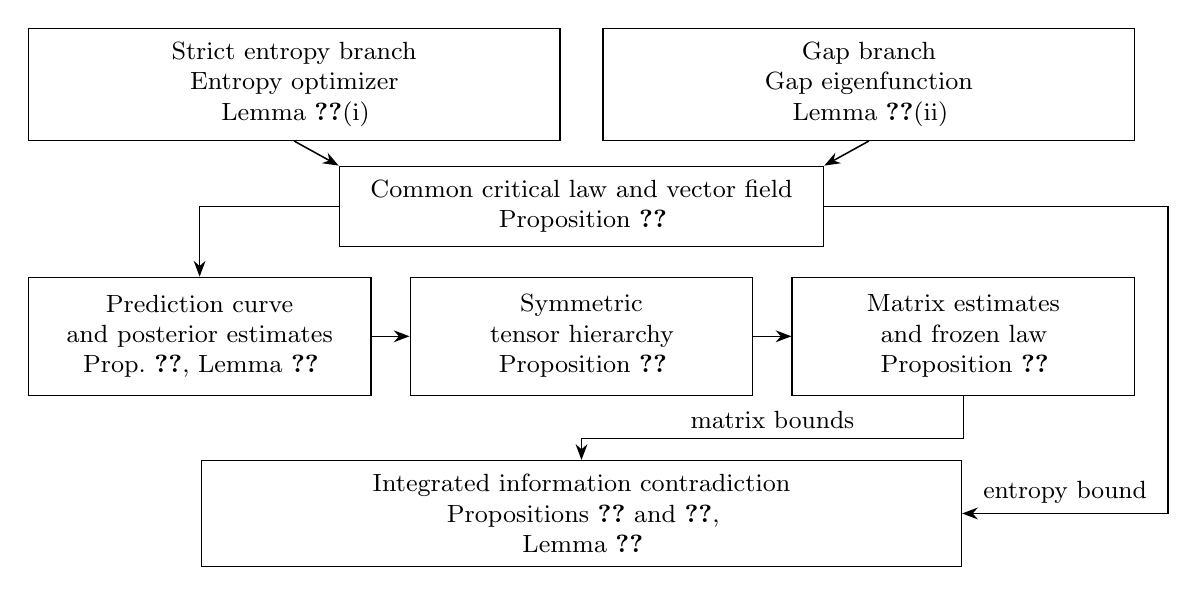
\begin{tikzpicture}[
  font=\small,
  stage/.style={draw, line width=.45pt, align=center,
    inner xsep=5pt, inner ysep=5pt},
  flow/.style={-{Stealth[length=2mm]}, line width=.55pt}
]
\node[stage, text width=6.4cm] (strict) at (-3.65,0)
  {Strict entropy branch\\
   Entropy optimizer\\
   Lemma~\ref{lem:critical-two-alternatives}(i)};
\node[stage, text width=6.4cm] (gap) at (3.65,0)
  {Gap branch\\
   Gap eigenfunction\\
   Lemma~\ref{lem:critical-two-alternatives}(ii)};

\node[stage, text width=5.8cm] (critical) at (0,-1.55)
  {Common critical law and vector field\\
   Proposition~\ref{prop:critical-sequence}};
\draw[flow] (strict.south) -- (critical.north west);
\draw[flow] (gap.south) -- (critical.north east);

\node[stage, text width=4.0cm, minimum height=1.5cm]
  (prediction) at (-4.85,-3.2)
  {Prediction curve\\
   and posterior estimates\\
   Prop.~\ref{prop:prediction}, Lemma~\ref{lem:posterior-outliers}};
\node[stage, text width=4.0cm, minimum height=1.5cm]
  (hierarchy) at (0,-3.2)
  {Symmetric\\tensor hierarchy\\
   Proposition~\ref{prop:hierarchy}};
\node[stage, text width=4.0cm, minimum height=1.5cm]
  (matrix) at (4.85,-3.2)
  {Matrix estimates\\and frozen law\\
   Proposition~\ref{prop:frozen-law}};
\draw[flow] (critical.west) -| (prediction.north);
\draw[flow] (prediction.east) -- (hierarchy.west);
\draw[flow] (hierarchy.east) -- (matrix.west);

\node[stage, text width=9.3cm] (contradiction) at (0,-5.45)
  {Integrated information contradiction\\
   Propositions~\ref{prop:information-upper}
   and~\ref{prop:information-lower},\\
   Lemma~\ref{lem:scalar-divergence}};
\draw[flow] (matrix.south) -- (4.85,-4.5)
  -- node[above, align=center] {matrix bounds} (0,-4.5)
  -- (contradiction.north);
\draw[flow] (critical.east) -- (7.45,-1.55)
  -- (7.45,-5.45)
  -- node[above, align=center] {entropy bound} (contradiction.east);
\end{tikzpicture}
\caption{Main stages of the contradiction argument. At the regularized
law, the strict entropy branch means that the logarithmic Sobolev
constant exceeds the Poincar\'e constant; in the gap branch the two
constants coincide. The logarithmic Sobolev inequality of the common
critical law, together with the square-root energy estimates of
Section~\ref{sec:matrices}, supplies the information upper bound.
The frozen matrix law supplies the scalar lower bound. After the
sequence limit at fixed parameters, its scale integral becomes
arbitrarily large as the diffusion time and covariance cap grow together.}
\label{fig:proof-dependencies}
\end{figure}


\subsection{Components of the argument}

Two ingredients have formulations beyond the final contradiction.
The entropy-loss comparison of Lemma~\ref{lem:entropy-loss} relates
relative entropy under common Gaussian convolution to conditional
prediction of the original relative score.  Its proof separates
the convexity input from the finite-copy observation argument.
The matrix reduction in Section~\ref{sec:matrices} converts symmetric
tensor near-equalities into a weighted scalar fluctuation law,
without requiring simultaneous diagonalization in varying
dimensions.  Section~\ref{sec:observations} then tests that law through
bounded covariance observations and integrates over scale.

For orientation, Section~\ref{sec:calculus} records the analytic
conventions and approximation facts.
Section~\ref{sec:critical} constructs the critical laws and vector
fields.
Section~\ref{sec:prediction} proves the prediction identity,
and Section~\ref{sec:hierarchy} constructs the tensor hierarchy.
Sections~\ref{sec:matrices} and \ref{sec:observations} turn that
hierarchy into the contradiction.


\newpage
\section{Curvature, diffusion, and entropy calculus}\label{sec:calculus}

We first establish the analytic facts used to construct and study the
probability measures in the proof. Two time conventions will be kept
distinct: convolution with a Gaussian of variance $r$ has generator
$\Delta/2$, whereas a stationary diffusion has generator $-A$ and noise
coefficient $\sqrt2$. These conventions determine every entropy
dissipation factor below.

For probabilities $p,\pi$ with $p\ll\pi$, define their relative entropy by
\[
 H(p\mid\pi)=\int\log\frac{dp}{d\pi}\,dp.
\]
Set $H(p\mid\pi)=+\infty$ when absolute continuity fails. Write
$\gamma$ for standard Gaussian measure in the relevant dimension, and set
\[
 \Ical(p\mid\pi)=4\int\left|D\sqrt{\frac{dp}{d\pi}}\right|^2d\pi.
\]
The value is $+\infty$ unless the density exists and its square root
belongs to the weighted Sobolev space. When the densities are positive
and smooth this is $\int|D\log(dp/d\pi)|^2dp$. Our convention is
\[
 \Ent_\pi(f^2)\le 2R(\pi)\int|Df|^2d\pi,
 \qquad 2H(p\mid\pi)\le R(\pi)\Ical(p\mid\pi).
\]
The Poincar\'e constant $R^P(\pi)$ uses the convention
\[
 \Var_\pi(f)=\int f^2d\pi-\left(\int f\,d\pi\right)^2
 \le R^P(\pi)\int|Df|^2d\pi.
\]
Linearization of the entropy inequality gives $R^P(\pi)\le R(\pi)$.

For smooth positive densities the Sobolev space is the completion of
$C_c^\infty$ in the squared norm $\int(f^2+|Df|^2)d\pi$.
Cutoffs, truncation of the values, and smoothing on compact sets show
that it also consists of the functions with a weak gradient in this
norm. The same approximation and lower semicontinuity of entropy
extend a compact-test logarithmic Sobolev inequality to this space.
One convenient proof of the latter lower semicontinuity is the formula
\begin{equation}\label{eq:calculus-entropy-duality}
 H(p\mid\pi)=\sup_{g\ \mathrm{bounded}}
 \left\{\int g\,dp-\log\int e^g d\pi\right\}.
\end{equation}
Jensen's inequality proves the upper bound; bounded truncations of
$\log(dp/d\pi)$ give equality. The same formula implies data
processing under a measurable map or a Markov kernel, by conditional
Jensen. Conditional entropy identities below are always averaged over
the conditioning variable. In particular, disintegrating a joint
density and splitting its logarithm gives the chain rule
\[
 H(P_{U,Z}\mid Q_U\otimes\nu)
 =H(P_U\mid Q_U)+\E_{P_U}H(P_{Z\mid U}\mid\nu).
\]
It holds in the extended nonnegative sense by truncation. Mutual
information is $\MI(U;Z)=H(P_{U,Z}\mid P_U\otimes P_Z)$.
Taking $g(z)=v\cdot z$ in Equation~\eqref{eq:calculus-entropy-duality}
and optimizing over $v$ also gives
$H(p\mid\gamma)\ge|\E_pZ|^2/2$ when the mean exists.

The following is the anisotropic Bakry--\'Emery curvature criterion
\cite{BakryEmery1985}.  We include its semigroup proof and the convex
approximation needed for Gaussian posteriors with nonsmooth support.

\begin{lemma}[Positive curvature]\label{lem:curvature}
Let $S$ be a positive definite matrix on $\R^n$, and let $U$ be a
proper lower semicontinuous convex function, possibly taking the value
$+\infty$. Suppose
\[
 d\pi(x)=Z^{-1}\exp\{-\tfrac12\langle x,Sx\rangle-U(x)\}\,dx
\]
is a probability with a full dimensional support. Then
\[
 \Ent_\pi(f^2)\le2\E_\pi\langle Df,S^{-1}Df\rangle,
 \qquad
 \Var_\pi(f)\le\E_\pi\langle Df,S^{-1}Df\rangle.
\]
The inequalities hold first for compact smooth tests, and then for
functions obtained by finite-energy approximation.
\end{lemma}

\begin{proof}
A linear change of variables reduces the assertion to $S=\Id$.
First suppose $V(x)=|x|^2/2+U(x)$ is smooth with bounded Hessian.
The diffusion with generator $L=\Delta-DV\cdot D$ has globally
Lipschitz drift and invariant law $\pi$. If $J_t$ is the derivative
of its trajectory with respect to the starting point, then
$\dot J_t=-D^2V(X_t)J_t$, whence $\|J_t\|_{\op}\le e^{-t}$.
For smooth bounded positive $q$, bounded away from zero,
weighted Cauchy--Schwarz gives
\[
 \frac{|DP_tq|^2}{P_tq}
 \le e^{-2t}P_t\left(\frac{|Dq|^2}{q}\right).
\]
Integration by parts yields
\[
 \frac{d}{dt}\int (P_tq)\log(P_tq)\,d\pi
 =-\int\frac{|DP_tq|^2}{P_tq}\,d\pi.
\]
Couple a trajectory started at $x$ to an independent stationary
initial point with the same driving Brownian motion. Their distance
is at most $e^{-t}$ times their initial distance. Since $\pi$ has
Gaussian tails, this proves convergence of $P_tq$ to $\E_\pi q$
for bounded Lipschitz $q$, and hence convergence of its entropy to
zero. Integrating the preceding two displays gives
$\Ent_\pi(q)\le\frac12\int|Dq|^2/q\,d\pi$. Apply this to
$q=f^2+\varepsilon$ and let $\varepsilon\downarrow0$.

For general $U$, take its quadratic infimal convolutions
\[
 U_j(x)=\inf_z\{U(z)+j|x-z|^2\}.
\]
The minimizer is unique, and monotonicity of the subgradient of $U$
shows that $DU_j$ is Lipschitz. The functions $U_j$ are convex and
increase to $U$. A fixed affine minorant $U(z)\ge\ell\cdot z+c$
gives $U_j(x)\ge\ell\cdot x+c-|\ell|^2/(4j)$.
Mollify $U_j$ with a smooth compactly supported kernel at radii
tending to zero. The resulting functions are smooth, convex, and
have bounded Hessian; the affine lower bound persists with a
uniform additive error. Consequently their normalized densities
converge almost everywhere and in $L^1$, dominated by an integrable
Gaussian times an exponential of a linear function. The compact-test
inequality passes to the limit. Boundary values of $U$ do not matter,
since the boundary of a full dimensional convex support has
Lebesgue measure zero. Finally, insert $f=1+\varepsilon g$,
using finite-energy cutoffs of the constant, and compare the
coefficients of $\varepsilon^2$ to obtain the variance inequality.
\end{proof}

We shall also use two immediate consequences with their constants.
If independent laws satisfy inequalities with quadratic energy
forms $Q_1,Q_2$, their product satisfies the inequality with energy
$Q_1+Q_2$. Indeed, decompose entropy into conditional entropy and
the entropy of the fiber integral, and use
\[
 \left|D_x\left(\int f(x,y)^2d\pi_2(y)\right)^{1/2}\right|^2
 \le\int|D_xf(x,y)|^2d\pi_2(y).
\]
Approximation removes zeros of the fiber norm. The variance version
uses conditional variance and differentiation of the fiber mean.
In particular, independent addition gives
\begin{equation}\label{eq:calculus-convolution}
 R(\Law(X+Z))\le R(\Law(X))+R(\Law(Z)).
\end{equation}
Second, Herbst's argument (see \cite[Section~2.3]{Ledoux1999})
shows that, if $R(\pi)\le R$, every integrable $1$-Lipschitz function
$u$ satisfies
\begin{equation}\label{eq:calculus-herbst}
 \log\E_\pi e^{t(u-\E_\pi u)}\le Rt^2/2.
\end{equation}
For a bounded smooth $u$, applying the inequality to $e^{tu/2}$,
and writing $\psi(t)=\log\E e^{tu}$, gives
$t\psi'(t)-\psi(t)\le Rt^2/2$. Integrate the derivative of
$\psi(t)/t$ from zero. Bounded Lipschitz truncations and Fatou's
lemma prove the assertion in general. In particular the conclusion
applies to linear forms whenever their first moments are finite.

\begin{lemma}[Dirichlet operator and stationary diffusion]
\label{lem:dirichlet-core}
Let $\pi$ be a smooth, strictly positive probability density on
$\R^n$. On $C_c^\infty(\R^n)$ define
\[
 A_\pi=-\Delta-D\log\pi\cdot D.
\]
This nonnegative symmetric operator is essentially self-adjoint in
$L^2(\pi)$, and $C_c^\infty$ is a core for its closure. In
particular, if $f\in L^2(\pi)$ and the distribution $A_\pi f$
belongs to $L^2(\pi)$, then $f\in\Dom(A_\pi)$. Its semigroup
$P_u=e^{-uA_\pi}$ preserves constants and is realized by the
stationary diffusion
\begin{equation}\label{eq:calculus-diffusion}
 dY_u=\sqrt2\,dB_u+D\log\pi(Y_u)\,du,
 \qquad Y_0\sim\pi.
\end{equation}
For $f\in\Dom(A_\pi)$ the stationary It\^o formula holds in $L^2$,
with drift $-A_\pi f$ and martingale integrand $\sqrt2\,Df$.
\end{lemma}

\begin{proof}
Integration by parts gives
$\langle f,A_\pi g\rangle=\int Df\cdot Dg\,d\pi$.
If $v\in L^2(\pi)$ is orthogonal to
$(1+A_\pi)C_c^\infty$, then $(1+A_\pi)v=0$
distributionally.  Conjugating by $\sqrt\pi$ reduces this to a
Poisson equation with a smooth local potential.  The local Newtonian
potential estimates and bootstrap make $v$ smooth; see
\cite[Lecture~24, p.~2; Lecture~16, p.~2]{Viaclovsky2004}. Take a compact cutoff $\chi_R$, equal to one on the ball
of radius $R$, with $|D\chi_R|\le C/R$. Testing by
$\chi_R^2v$ and using $2ab\le a^2/2+2b^2$ gives
\[
 \int\chi_R^2v^2d\pi+\tfrac12\int\chi_R^2|Dv|^2d\pi
 \le2\int|D\chi_R|^2v^2d\pi.
\]
Thus $v=0$. The range of $1+A_\pi$ is dense. Nonnegativity
gives $\|(1+A_\pi)f\|_2\ge\|f\|_2$, so the range of the
closure is also closed and therefore equals $L^2$. The closure is
self-adjoint: for $g$ in its adjoint domain, solve
$(1+\overline A)h=(1+A^*)g$; then $g-h$ is in the orthogonal
complement of the range of $1+A$, hence vanishes. This also proves
the asserted maximal distributional domain characterization.

The cutoffs $\chi_R$ converge to $1$ in the form norm with energy
tending to zero. Hence $1$ belongs to the nullspace of the closed
form and $P_u1=1$. To identify the diffusion, solve the stochastic
equation locally and kill it on exiting each ball. Its kernels are
symmetric and sub-Markov, as follows either from the Dirichlet
heat equation or integration by parts. Increasing the balls gives
the minimal sub-Markov semigroup. The stopped It\^o formula on
compact tests identifies its generator as an extension of $-A_\pi$.
Essential self-adjointness identifies it with $P_u$, which loses
no mass. Started in $\pi$, the resulting diffusion is stationary
and nonexplosive. Finally approximate $f$ in graph norm by compact
smooth functions. Their gradients converge in $L^2(\pi)$ since
$\|Dg\|_2^2=\langle g,Ag\rangle$. Stationarity and the
It\^o isometry pass every term of their formulas to the limit.
\end{proof}

\begin{lemma}[Entropy dissipation]\label{lem:entropy-calculus}
For the semigroup of Lemma~\ref{lem:dirichlet-core}, if
$p_0=q_0\pi$ has finite relative entropy and
$p_u=(P_uq_0)\pi$, then, for $0\le a\le b$,
\begin{equation}\label{eq:calculus-stationary-entropy}
 H(p_a\mid\pi)-H(p_b\mid\pi)
 \ge\int_a^b\Ical(p_u\mid\pi)\,du.
\end{equation}
If instead both probability measures evolve by Gaussian convolution,
$p_r=p_0*\gamma_r$ and $q_r=q_0*\gamma_r$, then
\begin{equation}\label{eq:calculus-heat-entropy}
 H(p_a\mid q_a)-H(p_b\mid q_b)
 \ge\frac12\int_a^b\Ical(p_r\mid q_r)\,dr
\end{equation}
whenever the entropy on the left at time $a$ is finite. Here
$\gamma_r$ is the centered Gaussian with covariance $r\Id$,
and time zero is allowed. For the standard Gaussian
Ornstein--Uhlenbeck semigroup, Equation~\eqref{eq:calculus-stationary-entropy}
is an equality, including time zero when the initial entropy is
finite. Each assertion also holds after integration over conditioning
labels whose noises are independent conditional on those labels.
\end{lemma}

\begin{proof}
For a bounded density $q$ bounded away from zero, the form chain
rule, first for smooth functions and then by form approximation,
gives
\[
 \frac{d}{du}\int(P_uq)\log(P_uq)\,d\pi
 =-\int\frac{|DP_uq|^2}{P_uq}\,d\pi.
\]
Spectral smoothing puts $P_uq$ in the operator domain for $u>0$;
the bounded range permits $1+\log(P_uq)$ as a form test.
Approximate an arbitrary finite-entropy density by truncating it
above and below and normalizing. The initial entropies converge.
The semigroup contracts $L^1$, so densities converge at every
later time. Lower semicontinuity of entropy and of
$4\int|D\sqrt q|^2d\pi$, followed by Fatou's lemma in time,
gives Equation~\eqref{eq:calculus-stationary-entropy} from time zero.
Restarting the argument gives arbitrary $a$.

For simultaneous heat evolution put $z=p_r/q_r$. Direct
differentiation, using $\partial_r p_r=\Delta p_r/2$ and the
same equation for $q_r$, gives
\begin{equation}\label{eq:calculus-heat-chain}
 (\partial_r-\tfrac12\Delta)\{q_r\Phi(z)\}
 =-\tfrac12q_r\Phi''(z)|Dz|^2.
\end{equation}
Here use smooth convex $\Phi_k$ with
$\Phi_k(1)=\Phi_k'(1)=0$, with second derivatives increasing to
$1/z$, and with second derivatives supported in compact subsets
of $(0,\infty)$. Such functions have at most linear growth and
increase to $z\log z-z+1$. Integrate
Equation~\eqref{eq:calculus-heat-chain} against $\chi_R$ with
$|\Delta\chi_R|\le C/R^2$. At each fixed $k$ the cutoff error
vanishes because $q_r\Phi_k(p_r/q_r)\le C_k(p_r+q_r)$.
Let $R\to\infty$ and then $k\to\infty$. Monotone convergence
gives the entropy and information terms, and in particular the
stated inequality on positive time intervals. Data processing
gives $H(p_\varepsilon\mid q_\varepsilon)\le H(p_0\mid q_0)$;
let $\varepsilon\downarrow0$ to include the initial time.

For Ornstein--Uhlenbeck evolution relative to $\gamma$, apply
the same convex truncations to the ratio. Its generator is
$\Delta-x\cdot D$. Expanding radial cutoffs have bounded
generator, tending pointwise to zero, so the error vanishes by
domination at fixed $k$. This gives equality on positive time
intervals. At time zero, relative entropy is continuous: data
processing gives its upper bound and lower semicontinuity under
weak convergence gives its lower bound. Monotone convergence of
the nonnegative time integral includes zero. Tonelli's theorem
proves all conditional versions.
\end{proof}

We use the relative-entropy form of the Gaussian-channel identity of
Guo, Shamai, and Verd\'u \cite[Theorem~5, Equation~(66)]{GuoShamaiVerdu2005}.
The proof records explicitly its conditional integrated form.

\begin{lemma}[Gaussian signals]\label{lem:gaussian-signals}
Let $S$ be an $\R^d$-valued random vector with finite second
moment, let $U$ be any side information, and let $G$ be standard
Gaussian independent of $(S,U)$. Write $Z_t=\sqrt tS+G$ and
\[
 d(t)=\E_U H(\Law(Z_t\mid U)\mid\gamma).
\]
Then $d(0)=0$, $d(t)\le t\E|S|^2/2$, and
\begin{equation}\label{eq:calculus-gaussian-signal}
 d(t)=\frac12\int_0^t
 \E\left|\E[S\mid Z_v,U]\right|^2dv.
\end{equation}
The integrand is nondecreasing in $v$. The formula without side
information is obtained by taking $U$ constant.
\end{lemma}

\begin{proof}
Conditional convexity of relative entropy and
$H(\gamma(\cdot-\sqrt t s)\mid\gamma)=t|s|^2/2$
give the upper bound. Gaussian kernel differentiation gives
\[
 D_z\log\frac{d\Law(Z_t\mid U)}{d\gamma}(z)
 =\sqrt t\,\E[S\mid Z_t=z,U].
\]
The differentiation is justified at each positive $t$ by the
Gaussian kernel and the finite second moment, or by truncating
$S$ and passing locally and in the conditional squared norm.
Applying Ornstein--Uhlenbeck evolution for time $u$ replaces $t$
by $te^{-2u}$. Its entropy dissipation identity and
$dt/du=-2t$ give $d'(t)=\frac12\E|\E[S\mid Z_t,U]|^2$
almost everywhere on $(0,\infty)$. The upper bound implies
$d(t)\to0$ at zero, proving the integrated identity. For
$0<v<t$, the channel at $v$ is obtained from the channel at $t$
by multiplying its output by $\sqrt{v/t}$ and adding fresh
Gaussian noise of covariance $(1-v/t)\Id$. Conditional Jensen
then proves monotonicity of prediction energy.
\end{proof}

\subsection{The transport--entropy consequence}
\label{sec:transport-consequence}

\begin{proof}[Proof of Corollary~\ref{cor:intro-transport}]
Jensen's inequality in each coordinate gives
$\int|x|^2d\mu\le na^2\log2$, so $\mu\in\mathcal P_2(\R^n)$.
Only the case $H(\nu\mid\mu)<\infty$ needs proof. For $s>0$, put
$\gamma_s=N(0,s\Id)$, $\mu_s=\mu*\gamma_s$, and
$\nu_s=\nu*\gamma_s$. The density of $\mu_s$ is smooth and strictly
positive. For $X\sim\mu$ and an independent standard Gaussian $G$,
its potential $V_s$ satisfies
\[
 D^2V_s(y)=s^{-1}\Id-s^{-2}\Cov(X\mid X+\sqrt sG=y)\ge0.
\]
Indeed, the posterior has the original convex potential plus
$|x-y|^2/(2s)$, so Lemma~\ref{lem:curvature} bounds its covariance
by $s\Id$. Gaussian differentiation is valid without compact support.
Thus $\mu_s$ is centered and log-concave, with a smooth convex potential.

Set $\beta_s=\sqrt{8s/3}$ and $a_s=a+\beta_s$. For a scalar standard
Gaussian $Z$, $\E\exp(sZ^2/\beta_s^2)=2$. The inequality
\[
 \frac{(u+t)^2}{(a+\beta_s)^2}
 \le\frac{a}{a+\beta_s}\frac{u^2}{a^2}
     +\frac{\beta_s}{a+\beta_s}\frac{t^2}{\beta_s^2}
\]
and H\"older's inequality show that $\mu_s$ satisfies
\eqref{eq:intro-subgaussian} with parameter $a_s$.
Theorem~\ref{thm:main}, with the Sobolev extension in
Section~\ref{sec:calculus}, gives entropy coefficient $Ca_s^2$.
In the conventions of \cite[Definitions~1--2]{OttoVillani2000},
$\Ent(f^2)\le L\int|Df|^2$ is $\mathrm{LSI}(2/L)$, whose
transport conclusion is $W_2^2\le LH$. Their Theorem~1 applies to
the smooth convex potential of $\mu_s$, and hence
\[
 W_2(\nu_s,\mu_s)^2\le Ca_s^2H(\nu_s\mid\mu_s)
 \le Ca_s^2H(\nu\mid\mu).
\]
The last inequality is data processing for the common Gaussian
kernel, as in Section~\ref{sec:calculus}. Coupling a vector with
itself plus independent Gaussian noise gives
$W_2(\mu_s,\mu),W_2(\nu_s,\nu)\le\sqrt{ns}$.
Letting $s\downarrow0$ at fixed $n$, with $a_s\to a$, proves the claim.
\end{proof}

\section{Critical laws after Gaussian regularization}\label{sec:critical}

Suppose that the conclusion of Theorem~\ref{thm:main} is false.
This section constructs, from a sequence of counterexamples, smooth
probabilities $\eta$ satisfying a logarithmic Sobolev inequality and
vector fields $w$ that nearly satisfy $A_\eta w=w$. There are two
possible constructions. An attained nonlinear entropy quotient gives
a score $w$; equality of the logarithmic Sobolev and Poincar\'e
constants gives the gradient of a gap eigenfunction. We shall retain
both alternatives throughout.

\subsection{Normalization and Gaussian regularization}

\begin{lemma}[Normalized counterexamples]\label{lem:critical-normalization}
Failure of Theorem~\ref{thm:main} produces a sequence of centered,
compactly supported, full dimensional log-concave probabilities $\mu$
such that
\begin{equation}\label{eq:critical-normalization}
 R(\mu)=1,\qquad
 \sup_{|\theta|=1}\E_\mu e^{\langle X,\theta\rangle^2/a^2}
 \le2,\qquad a\longrightarrow0.
\end{equation}
For an absolute constant $C$, they also satisfy
\begin{equation}\label{eq:critical-linear-mgf}
 \log\E_\mu e^{v\cdot X}\le Ca^2|v|^2,
 \qquad \Cov_\mu(X)\le Ca^2\Id.
\end{equation}
\end{lemma}

\begin{proof}
Choose laws and compact smooth tests for which the entropy-to-energy
ratio divided by the squared marginal parameter tends to infinity.
The tests may be chosen with positive energy: a smooth test of zero
energy is constant on the connected interior of the convex support,
and its entropy vanishes. Restriction of the law to a sufficiently
large ball preserves each test quotient arbitrarily closely. Multiply
the restricted density by $e^{-\varepsilon|x|^2/2}$ and normalize,
with $\varepsilon>0$ sufficiently small to preserve that quotient
again. Both operations preserve log-concavity, their combined density
relative to the original law can be bounded by $2$, and
Lemma~\ref{lem:curvature} gives a finite logarithmic Sobolev
constant for the resulting compact law.

A bounded density increase changes the exponential-square expectation
by at most that factor. If $\E e^{Z^2/A^2}\le4$, Jensen gives
$\E e^{Z^2/(2A^2)}\le2$. Centering costs only another absolute
factor: $\E Z^2\le A^2\log4$, while
$(Z-\E Z)^2\le2Z^2+2(\E Z)^2$; increase the denominator first
to make the resulting exponential expectation bounded by an absolute
constant, and once more by Jensen to make it at most $2$.
These arguments apply separately to every unit linear form with
the same constants. Translation preserves the test quotient. Thus
the centered compact laws still have $R/A^2\to\infty$ with
$0<R<\infty$. Dilation by $R^{-1/2}$ gives
Equation~\eqref{eq:critical-normalization}.

For completeness, if a centered scalar $Z$ obeys
$\E e^{Z^2/a^2}\le2$, then
$\E|Z|^k\le2a^k\Gamma(k/2+1)$, by integrating its tail.
Expansion of $e^{tZ}$, with the linear term absent, therefore gives
$\log\E e^{tZ}\le Ca^2t^2$ for $a|t|\le c$.
For $a|t|\ge c$, use
$tZ\le Z^2/a^2+a^2t^2/4$ and absorb $\log2$ into
$Ca^2t^2$. Apply this to $Z=X\cdot\theta$. The second moment
bound follows either from the exponential-square bound or by
differentiating the centered moment generating function at zero.
\end{proof}

We suppress the counterexample index, but all limits in this section
refer to this sequence. Let $G$ be a fresh standard Gaussian and set
\[
 \mu_s=\Law(X+\sqrt sG),\quad R_s=R(\mu_s),\quad
 b_s(y)=\E[X\mid X+\sqrt sG=y],\quad V_s=-\log\mu_s.
\]
Here and below $\mu_s$ also denotes its strictly positive density.
Gaussian differentiation and posterior covariance give
\begin{equation}\label{eq:critical-posterior}
 DV_s(y)=\frac{y-b_s(y)}s,\qquad
 M_s(y)=Db_s(y)=\frac{\Cov(X\mid y)}s,\qquad
 K_s(y)=D^2V_s(y)=\frac{\Id-M_s(y)}s.
\end{equation}
The posterior of $X$ has a convex potential plus $|x-y|^2/(2s)$.
Lemma~\ref{lem:curvature}, applied to its linear forms, therefore
implies
\begin{equation}\label{eq:critical-curvature}
 0\le M_s\le\Id,\qquad 0\le K_s\le s^{-1}\Id.
\end{equation}
All these functions are smooth. Compact support of $X$ also gives
$|b_s|\le\sup_{\supp\mu}|x|$.

The monotonicity below follows from the heat-flow contraction of
Klartag and Putterman \cite[Theorem~1.2 and Section~3]{KlartagPutterman2023},
which uses the transport construction of Kim and Milman
\cite{KimMilman2012}. We recall the argument for our regularized laws.

\begin{lemma}[Bounds for the regularized constants]
\label{lem:critical-flow-bounds}
The function $s\mapsto R_s$ is nondecreasing and $1$-Lipschitz on
$(0,\infty)$, and
\begin{equation}\label{eq:critical-basic-R}
 1\le R_s\le1+s.
\end{equation}
\end{lemma}

\begin{proof}
The heat equation for $\mu_s$ is the continuity equation with
velocity $DV_s/2$. On a compact positive-time interval this velocity
is globally Lipschitz and grows at most linearly, so its smooth flow
is a diffeomorphism carrying $\mu_s$ to $\mu_t$. Its Jacobian
satisfies $\dot J=K_tJ/2$. By positivity of $K_t$, the flow
expands distances and its inverse is $1$-Lipschitz when $t\ge s$.
Transport a test by that inverse. Its entropy is unchanged and
its Dirichlet energy cannot increase, proving $R_t\ge R_s$.
Equation~\eqref{eq:calculus-convolution} gives
$R_{s+h}\le R_s+h$ and $R_s\le1+s$. For every compact smooth
test, its entropy and energy converge to those under $\mu$ as
$s\downarrow0$. Taking the supremum of its quotient gives
$\liminf_{s\downarrow0}R_s\ge R(\mu)=1$. Monotonicity now
proves the remaining bound.
\end{proof}

\subsection{Attainment above the Gaussian and Poincar\'e thresholds}

On compact manifolds, Rothaus obtains nonconstant positive solutions
of the logarithmic Euler equation when the sharp logarithmic Sobolev
constant exceeds the Poincar\'e constant \cite[p.~358]{Rothaus1986}.
The proof below must also control loss of entropy in the Gaussian tails.
The next two lemmas establish this control and attainment. Their constants
may depend on a single fixed law and its dimension. Uniform estimates
along the counterexample sequence begin with the translation argument.

\begin{lemma}[Compactness and the Gaussian entropy defect]
\label{lem:critical-defect}
Fix $s>0$ and a compactly supported probability $\mu$ on $\R^n$,
and put $\nu=\mu*\gamma_s$. Its form domain embeds compactly
into $L^2(\nu)$. For every $\varepsilon>0$ there is a finite
$C_\varepsilon$, depending on this fixed law, such that
\begin{equation}\label{eq:critical-defective}
 \Ent_\nu(u^2)\le2(s+\varepsilon)\|Du\|_2^2
                  +C_\varepsilon\|u\|_2^2.
\end{equation}
If $u_j\to u$ in $L^2(\nu)$, $\|u_j\|_2=1$, and
$\|Du_j\|_2^2\to E_*<\infty$, then
\begin{equation}\label{eq:critical-entropy-defect}
 \limsup_j\Ent_\nu(u_j^2)
 \le\Ent_\nu(u^2)+2s(E_*-\|Du\|_2^2).
\end{equation}
\end{lemma}

\begin{proof}
Write $r=d\nu/d\gamma_s$. The Gaussian kernel formula gives
$D\log r=b_s/s$, which is bounded, and hence
$|\log r(y)|\le C(1+|y|)$. For $v=u\sqrt r$,
\[
 \Ent_\nu(u^2)=\Ent_{\gamma_s}(v^2)
                         -\int v^2\log r\,d\gamma_s,
 \qquad Dv=\sqrt r\,(Du+\tfrac12uD\log r).
\]
Gaussian integration by parts followed by Cauchy--Schwarz gives
\[
 \int |y|^2v^2d\gamma_s
 =sn\|v\|_2^2+2s\int v\,y\cdot Dv\,d\gamma_s
 \le2sn\|v\|_2^2+4s^2\|Dv\|_2^2.
\]
Initially this calculation is for compact tests, and cutoffs extend
it by lower semicontinuity. The linear-growth entropy correction
is consequently bounded by
$\delta\|Dv\|_2^2+C_\delta\|v\|_2^2$ for every $\delta>0$.
Gaussian logarithmic Sobolev and the displayed derivative formula,
with another arbitrarily small Cauchy--Schwarz parameter, prove
Equation~\eqref{eq:critical-defective}. The same moment estimate
shows tightness of the $L^2(\nu)$ mass of any bounded form
sequence. On a fixed ball, the smooth density is bounded above
and away from zero, so the ordinary local Rellich theorem gives
$L^2$ precompactness. A diagonal extraction and tightness prove
compactness globally.

We give the tail argument for the sharp coefficient $2s$ in
Equation~\eqref{eq:critical-entropy-defect}. Put
$v_{j,L}=(|u_j|-L)_+$ and $m_{j,L}=\|v_{j,L}\|_2^2$.
Strong $L^2$ convergence implies
$\lim_{L\to\infty}\sup_jm_{j,L}=0$. The energies of
$v_{j,L}$ and $|u_j|\wedge L$ sum to $\|Du_j\|_2^2$.
Lower semicontinuity for the clipped functions therefore gives
\begin{equation}\label{eq:critical-tail-energy}
 \lim_{L\to\infty}\limsup_j\|Dv_{j,L}\|_2^2
 \le E_*-\|Du\|_2^2.
\end{equation}
For a nonnegative $v$ of squared norm $m\le1$, the negative
part of $v^2\log v^2$ has integral at most $C\sqrt m$
(use $-z\log z\le C\sqrt z$ on $0\le z\le1$).
Since $m\log m\le0$, Equation~\eqref{eq:critical-defective}
thus gives
\[
 \int v^2\log_+v^2d\nu
 \le2(s+\varepsilon)\|Dv\|_2^2
          +C_\varepsilon m+C\sqrt m.
\]
If $|u_j|>ML$, where $M>1$ is fixed, then
$|u_j|\le c_M v_{j,L}$ with $c_M=M/(M-1)$. Consequently
\[
 u_j^2\log_+u_j^2
 \le c_M^2v_{j,L}^2\log_+v_{j,L}^2
                +c_M^2\log(c_M^2)v_{j,L}^2.
\]
The integrals of bounded truncations of $z^2\log z^2$ pass to
the limit by strong $L^2$ convergence; its negative part does as
well, being bounded and continuous. The last two bounds and
Equation~\eqref{eq:critical-tail-energy}, with limits in the order
$j$, $L$, $M$, $\varepsilon$, show that the lost positive
entropy is at most $2s(E_*-\|Du\|_2^2)$. The normalization
terms are zero because $\|u\|_2=\|u_j\|_2=1$.
\end{proof}

The threshold $s$ in the entropy-defect estimate controls escape into the
Gaussian tails.  The Poincar\'e constant controls maximizing sequences
that converge to constants.  The next lemma proves attainment when the
logarithmic Sobolev constant exceeds both thresholds.

\begin{lemma}[Existence and positivity of an optimizer]\label{lem:optimizer}
Let $\nu=\mu*\gamma_s$, where $s>0$ and $\mu$ is compactly
supported. Suppose its logarithmic Sobolev and Poincar\'e constants
$R=R(\nu)$ and $P=R^P(\nu)$ satisfy
$\infty>R>\max(P,s)$. Then there is a smooth strictly positive
nonconstant $f$ with
\begin{equation}\label{eq:critical-optimizer}
 \int f^2d\nu=1,\qquad
 \Ent_\nu(f^2)=2R\int|Df|^2d\nu,\qquad
 A_\nu f=\lambda f\log f,\quad\lambda=R^{-1}.
\end{equation}
The last equation is initially distributional and then classical.
\end{lemma}

\begin{proof}
Take nonnegative unit-norm maximizing tests $f_j$. Replacing a test
by its absolute value preserves entropy and energy, so this choice
loses nothing. Equation~\eqref{eq:critical-defective}, with
$s+\varepsilon<R$, bounds their energies. We first exclude
energies tending to zero; this is the only place the strict
inequality $R>P$ is required.

Suppose $\varepsilon_j^2=\|Df_j\|_2^2\to0$, and write
$c_j=\E_\nu f_j$ and $h_j=(f_j-c_j)/\varepsilon_j$.
Poincar\'e gives $\|h_j\|_2^2\le P$, while
$\|Dh_j\|_2^2=1$ and
$1-c_j^2=\varepsilon_j^2\|h_j\|_2^2$.
Thus $c_j\to1$. By compactness, after extraction,
$h_j\to h$ in $L^2$, where
\[
 \E h=0,\qquad \|Dh\|_2^2\le1,\qquad
 \|h\|_2^2\le P\|Dh\|_2^2.
\]
For $c>0$, $\varepsilon>0$ and $z\ge-c/\varepsilon$ define
\[
 Q_{c,\varepsilon}(z)=\varepsilon^{-2}
 \left[(c+\varepsilon z)^2\log\frac{(c+\varepsilon z)^2}{c^2}
                  -(c+\varepsilon z)^2+c^2\right].
\]
Normalization and $-\log c_j^2-1+c_j^2\ge0$ give
\begin{equation}\label{eq:critical-small-energy-start}
 \varepsilon_j^{-2}\Ent(f_j^2)
 \le\int Q_{c_j,\varepsilon_j}(h_j)\,d\nu.
\end{equation}
Here is the scalar estimate needed to control unbounded $h_j$.
For $1/2\le c\le1$ and $0<\varepsilon\le1/2$,
\begin{equation}\label{eq:critical-scalar-Q}
 0\le Q_{c,\varepsilon}(z)
 \le(2+2\log2)z^2+z^2\log_+z^2,
 \qquad Q_{c,\varepsilon}(z)\longrightarrow2z^2
\end{equation}
uniformly on bounded $z$-intervals as $c\to1$ and
$\varepsilon\to0$. To verify the bound, put $t=\varepsilon z/c$.
Then $Q=z^2B(t)$, where Taylor's integral formula gives
\[
 B(t)=2+4\int_0^1(1-r)\log(1+rt)\,dr,
 \qquad -1\le t<\infty.
\]
For $t\le0$, $B(t)\le2$. For $t\ge0$, use
$t\le z$ to obtain
$B(t)\le2+2\log(1+z)\le2+2\log2+\log_+z^2$.
Continuity at $t=0$ proves the compact convergence.

The tail proof in Lemma~\ref{lem:critical-defect} did not use
unit norm until its last sentence. In particular, for any bounded
form sequence $u_j\to u$ in $L^2$ with energies tending to $E_*$,
it proves
\begin{equation}\label{eq:critical-general-tail}
 \lim_{K\to\infty}\limsup_j
 \int_{|u_j|>K}u_j^2\log_+u_j^2d\nu
 \le2s(E_*-\|Du\|_2^2).
\end{equation}
Apply the compact convergence in Equation~\eqref{eq:critical-scalar-Q}
on $|h_j|\le K$ and its upper bound on the complement. Strong
$L^2$ convergence removes the quadratic tail as $K\to\infty$;
Equation~\eqref{eq:critical-general-tail} controls the entropy tail.
Equation~\eqref{eq:critical-small-energy-start} consequently gives
\[
 \limsup_j\varepsilon_j^{-2}\Ent(f_j^2)
 \le2\|h\|_2^2+2s(1-\|Dh\|_2^2)
 \le2\max(P,s)<2R.
\]
This contradicts the maximizing property.

We may therefore extract $f_j\to f$ strongly in $L^2$ with
$\|Df_j\|_2^2\to E_*>0$. Put $E=\|Df\|_2^2$. The entropy
defect and the sharp inequality give
\[
 2RE_*\le\Ent(f^2)+2s(E_*-E)
         \le2RE+2s(E_*-E).
\]
Since $R>s$ and $E\le E_*$, equality forces $E=E_*>0$.
Thus $f$ is a nonnegative, nonconstant optimizer.

The homogeneous functional
$\Ent(g^2)-2R\|Dg\|_2^2$ is nonpositive and is zero at $f$.
Its derivative along every compact smooth variation $\zeta$ is
\[
 4\int f\log f\,\zeta\,d\nu
       -4R\int Df\cdot D\zeta\,d\nu=0.
\]
The entropy normalization term cancels the additional linear term.
Differentiation is legitimate also at zeros because
$z^2\log z^2$ has derivative zero at zero. This proves the Euler
equation in Equation~\eqref{eq:critical-optimizer}.

We have obtained a nonnegative optimizer with positive energy.  To use
its logarithmic derivative, we still need local regularity and strict
positivity.  We spell out the weak-solution regularity step, using the
interior Newtonian-potential $L^p$ and Schauder estimates; see
\cite[Lecture~24, p.~2; Lecture~10, Proposition~1]{Viaclovsky2004}.
Write $\nu=e^{-V}$ and set $v=e^{-V/2}f\ge0$.  The function $V$ is smooth,
and direct differentiation of the weak equation gives
\[
 -\Delta v=\lambda v\log v+
 \left(\frac{\lambda V}{2}-\frac{|DV|^2}{4}
                         +\frac{\Delta V}{2}\right)v.
\]
The conjugating factor and its reciprocal are bounded on each fixed
ball.  Since $|z\log z|\le C_\delta(1+z^{1+\delta})$ for $z\ge0$,
local $L^p$ integrability of $v$ puts the right side in
$L^q_{\rm loc}$, where $q=p/(1+\delta)>1$.  Localize that right side
on a larger ball and take its Newtonian potential with the sign solving
$-\Delta u=F$.  The cited $L^q$ estimate gives $u\in W^{2,q}_{\rm loc}$;
the difference $v-u$ is distributionally harmonic and hence smooth by
Weyl's lemma \cite[Lecture~3, Theorem~2]{Viaclovsky2004}.
This proves the required $W^{2,q}$ gain directly for the weak solution.

For $n\ge2$, start with $p=2$ and choose
$0<\delta<\min(1,2/n)$.  Before boundedness is reached, Sobolev
embedding improves reciprocal integrability from $1/p$ to
$(1+\delta)/p-2/n$, a decrease greater than $1/n$ because $p\ge2$.
At a critical exponent use any sufficiently large finite integrability
exponent and continue once more.  After finitely many steps $q>n/2$,
so $v$, and thus $f$, is locally bounded and H\"older continuous.
In dimension one the same conclusion follows by twice integrating the
local Poisson equation.  The function $z\log z$ is locally H\"older
of every exponent below one on $[0,\infty)$; reducing the exponent
if necessary, the Schauder estimate therefore gives
$f\in C^{2,\alpha}_{\rm loc}$ for some $\alpha>0$.
All constants in this paragraph concern one fixed law and dimension;
none enters a uniform estimate along the counterexample sequence.

If $f(x_0)=0$, choose a ball $B$ about $x_0$ with
$0\le f\le b<1$ on its closure. Start the $\nu$-diffusion at
$x_0$ and stop at its exit time $\tau$ from $B$. For
$Z_t=f(Y_{t\wedge\tau})$, $m(t)=\E Z_t$, and
$g(z)=-\lambda z\log z$, the stopped It\^o formula gives, for almost
every $t$,
\[
 m'(t)=\E[\1_{t<\tau}g(Z_t)]\le\E g(Z_t)\le g(m(t)),
 \qquad m(0)=0.
\]
Indeed $g$ is nonnegative and concave on $[0,b]$; the first
inequality adds its nonnegative stopped boundary contribution.
Also $m'\ge0$. If $m(t_1)>0$, let $t_a$ be the first time at
which $m=a$, for $0<a<m(t_1)$. Integration gives
\[
 \int_a^{m(t_1)}\frac{dz}{-\lambda z\log z}
 \le t_1-t_a\le t_1,
\]
contradicting divergence as $a\downarrow0$. Hence $m=0$.
The killed nondegenerate diffusion has positive probability of
reaching each open subset of $B$ while staying in $B$: one can
follow a smooth interior path by requiring Brownian motion to
remain in a small tube about its corresponding driving path,
and use local Lipschitz continuity of the drift. Brownian tube
probabilities are positive by its finite increment densities and
bridge continuity. Consequently $f$ vanishes throughout $B$.
Its zero set is both open and closed, impossible in connected
$\R^n$ for a unit-norm function. Thus $f>0$, and smooth elliptic
bootstrap makes $f$ smooth everywhere.
\end{proof}

An optimizer supplies a second probability with its own logarithmic
Sobolev inequality. The next identity explains why no convexity
assumption on this second probability is needed.

\begin{samepage}
\begin{lemma}[Change of reference at an optimizer]
\label{lem:critical-change-reference}
Under Lemma~\ref{lem:optimizer}, suppose in addition that
$\nu=e^{-V}$ is log-concave with bounded $K=D^2V$.
Define
\[
 \eta=f^2\nu,\qquad h=\log f^2,\qquad w=Dh,\qquad
 I=\E_\eta|w|^2.
\]
Then $I=2\lambda H(\eta\mid\nu)>0$, $R(\eta)\le1/\lambda$,
each component of $w$ belongs to $\Dom(A_\eta)$, and
\begin{equation}\label{eq:critical-score-equation}
 A_\nu h=\lambda h+\tfrac12|w|^2,
 \qquad A_\eta w=(\lambda\Id-K)w.
\end{equation}
Moreover,
\begin{equation}\label{eq:critical-curvature-mean}
 \E_\eta\langle w,Kw\rangle\le\lambda|\E_\eta w|^2.
\end{equation}
\end{lemma}
\end{samepage}

\begin{proof}
Since $w=2Df/f$, $I=4\|Df\|_{L^2(\nu)}^2$; optimizer
equality gives $I=2\lambda H(\eta\mid\nu)>0$.
The chain rule applied to its Euler equation gives the first
identity in Equation~\eqref{eq:critical-score-equation}. Commuting
one derivative with $A_\nu$ gives
\[
 A_\nu w=D(A_\nu h)-Kw
       =\lambda w+(Dw)w-Kw.
\]
Since $A_\eta=A_\nu-w\cdot D$ and $Dw$ is symmetric, the
second identity follows distributionally. Its right side is in
$L^2(\eta)$, since $K$ is bounded and $w\in L^2(\eta)$.
Lemma~\ref{lem:dirichlet-core} therefore puts $w$ in the
operator domain; no unproved integrability of higher derivatives
has been used.

Let $p=g^2\eta$ have unit mass, where $g$ is compactly supported
and smooth. Direct expansion and compactly supported integration
by parts give
\begin{align*}
 \Ical(p\mid\nu)
 &=\Ical(p\mid\eta)+\int g^2|w|^2d\eta
                    +2\int D(g^2)\cdot w\,d\eta\\
 &=\Ical(p\mid\eta)+\int g^2\{|w|^2+2A_\eta h\}\,d\eta\\
 &=\Ical(p\mid\eta)+2\lambda\int h\,dp.
\end{align*}
These formulas may be read in square-root form at zeros of $g$.
On the other hand
$H(p\mid\nu)=H(p\mid\eta)+\int h\,dp$. Thus
\begin{equation}\label{eq:critical-exact-deficit}
 \Ical(p\mid\nu)-2\lambda H(p\mid\nu)
 =\Ical(p\mid\eta)-2\lambda H(p\mid\eta).
\end{equation}
Apply the inequality for $\nu$ to the compact smooth function
$gf$. Its deficit is nonnegative, so the right side is
nonnegative. Homogeneity and the Sobolev approximation of
Section~\ref{sec:calculus} prove $R(\eta)\le1/\lambda$.
Finally the domain identity gives
\[
 \E_\eta|Dw|^2=\lambda I-\E_\eta\langle w,Kw\rangle,
\]
while Poincar\'e for $\eta$ gives the lower bound
$\lambda(I-|\E_\eta w|^2)$. Subtract to obtain
Equation~\eqref{eq:critical-curvature-mean}.
\end{proof}

\subsection{Uniform estimates in the two alternatives}

\begin{lemma}[Translation gain]\label{lem:translation-gain}
Let $\mu$ satisfy Equation~\eqref{eq:critical-normalization}, with
$a\le1$. Fix a compact interval $J\subset(0,1/2)$. There is a
constant $C_J$, independent of the dimension and of the support
radius of $\mu$, with the following property. For $s\in J$, put
$\lambda=R_s^{-1}$. If $\sigma$ is any probability with
\[
 D_0=H(\sigma\mid\mu_s)<\infty,\qquad
 F_0=\Ical(\sigma\mid\mu_s)<\infty,\qquad p=\E_\sigma Y,
\]
then
\begin{equation}\label{eq:critical-translation-gain}
 F_0-2\lambda D_0
 \ge(s^{-2}-\lambda/s)|p|^2
                   -C_J\sqrt a\,(F_0+D_0).
\end{equation}
\end{lemma}

\begin{proof}
The centered linear moment generating functions under $\mu_s$
obey
\[
 \log\E_{\mu_s}e^{v\cdot Y}\le C_J|v|^2,
 \qquad
 \log\E_{\mu_s}e^{v\cdot b_s(Y)}\le Ca^2|v|^2.
\]
The first follows by independent Gaussian addition and
Equation~\eqref{eq:critical-linear-mgf}; the second follows by
conditional Jensen from that equation. Entropy duality, optimized
over the scalar multiple of each unit vector, gives
\begin{equation}\label{eq:critical-entropic-means}
 |p|\le C_J\sqrt{D_0},\qquad
 |\E_\sigma b_s(Y)|\le Ca\sqrt{D_0}.
\end{equation}
All expectations exist. More explicitly, compact support of $X$
makes $\E_{\mu_s}e^{c|Y|^2}<\infty$ for some $c>0$;
entropy duality then implies $\E_\sigma|Y|^2<\infty$.
The latter fact is used only for integrability, not for a uniform
bound in dimension.

Let $\sigma_u$ be the translate of $\sigma$ by $-up$,
$0\le u\le1$, and let $D_u=H(\sigma_u\mid\mu_s)$.
Change of variables in entropy and the Hessian bound give
\begin{align*}
 D_u
 &=D_0+\E_\sigma[V_s(Y-up)-V_s(Y)]\\
 &\le D_0-u|p|^2/s+u\,p\cdot\E_\sigma b_s(Y)/s
                                +u^2|p|^2/(2s)
 \le C_JD_0.
\end{align*}
Thus Equation~\eqref{eq:critical-entropic-means}, applied to
$\sigma_u$, implies
$|\E_\sigma b_s(Y-up)|\le C_Ja\sqrt{D_0}$ uniformly in $u$.
Differentiating the exact entropy expression, and then integrating,
gives
\begin{equation}\label{eq:critical-translated-entropy}
 D_1=D_0-\frac{|p|^2}{2s}+O_J(aD_0).
\end{equation}
Indeed its derivative is
$-(1-u)|p|^2/s+p\cdot\E_\sigma b_s(Y-up)/s$.

Write $r(Y)=D\log(d\sigma/d\mu_s)(Y)$ in the weak
square-root sense. Its mean is
\begin{equation}\label{eq:critical-score-mean}
 \E_\sigma r=\E_\sigma DV_s=(p-\E_\sigma b_s)/s.
\end{equation}
To justify this for finite Fisher information, the Lebesgue density
$q$ of $\sigma$ has weak derivative
$Dq=q(r-DV_s)\in L^1$: $r$ is square integrable and $DV_s$
has linear growth. Integrating against expanding cutoffs gives
$\int Dq=0$ and hence Equation~\eqref{eq:critical-score-mean}.

In the moving coordinates $Y$, the score of $\sigma_1$ relative
to $\mu_s$ is
\[
 r(Y)-p/s+d(Y)/s,\qquad d(Y)=b_s(Y)-b_s(Y-p).
\]
Since $0\le Db_s\le\Id$, integration along the segment gives
\[
 |d(Y)|^2
 =\left|\int_0^1M_s(Y-up)p\,du\right|^2
 \le\int_0^1|M_s(Y-up)p|^2du
 \le p\cdot d(Y).
\]
The mean estimates at the two endpoints therefore imply
\begin{equation}\label{eq:critical-posterior-translation-error}
 \E_\sigma|d|^2\le C_JaD_0.
\end{equation}
Expanding the score square and using
Equation~\eqref{eq:critical-score-mean},
\[
 \E_\sigma|r-p/s|^2
 =F_0-|p|^2/s^2+2p\cdot\E_\sigma b_s/s^2.
\]
The remaining cross term is bounded by
$C_J\sqrt{aD_0}\,(\sqrt{F_0}+\sqrt{D_0})$, and the
$d$-square term by $C_JaD_0$. Consequently the translated
information is finite and satisfies
\begin{equation}\label{eq:critical-translated-information}
 F_1=F_0-|p|^2/s^2+O_J(\sqrt a\,(F_0+D_0)).
\end{equation}
These calculations require only the weak derivatives already
justified, so they apply also when the density of $\sigma$ vanishes.
Apply logarithmic Sobolev to $\sigma_1$, namely
$F_1\ge2\lambda D_1$, and combine
Equations~\eqref{eq:critical-translated-entropy} and
\eqref{eq:critical-translated-information}. Since
$2/3\le\lambda\le1$ on the time interval in question, this
proves Equation~\eqref{eq:critical-translation-gain}.
\end{proof}

We can now obtain estimates that are uniform along the counterexample
sequence. Write $R_s^P$ for the optimal Poincar\'e constant of
$\mu_s$. By linearization $R_s^P\le R_s$. Since $R_s\ge1>s$
on $(0,1/2)$, the strict alternative $R_s>R_s^P$ meets all
the hypotheses of Lemma~\ref{lem:optimizer}.

\begin{lemma}[Critical fields in both alternatives]
\label{lem:critical-two-alternatives}
Fix $J\subset(0,1/2)$ compact and $s\in J$, and put
$\lambda=1/R_s$. There are a smooth positive probability $\eta$
and a smooth vector field $w$, with
$0<I:=\E_\eta|w|^2<\infty$, such that
\begin{equation}\label{eq:critical-common-identities}
 R(\eta)\le\lambda^{-1},\qquad
 w\in\Dom(A_\eta)^n,\qquad
 A_\eta w=(\lambda\Id-K_s)w.
\end{equation}
They can be chosen as follows.
\begin{enumerate}[label=\textup{(\roman*)}]
\item If $R_s>R_s^P$, take the optimizer $f$ of
Lemma~\ref{lem:optimizer} and set
\[
 \eta=f^2\mu_s,\qquad w=D\log f^2,
 \qquad I=2\lambda H(\eta\mid\mu_s).
\]
\item If $R_s=R_s^P$, there is a centered nonconstant gap
eigenfunction $\varphi$ satisfying
$A_{\mu_s}\varphi=\lambda\varphi$. Take
\[
 \eta=\mu_s,\qquad w=D\varphi,
 \qquad I=\lambda\E_{\mu_s}\varphi^2.
\]
\end{enumerate}
In either alternative,
\begin{equation}\label{eq:critical-uniform-smallness}
 |\E_\eta w|^2+\E_\eta|K_sw|^2\le C_J\sqrt a\,I,
 \qquad
 \E_\eta\langle w,K_sw\rangle\le\lambda|\E_\eta w|^2.
\end{equation}
In alternative \textup{(ii)} the factor $\sqrt a$ can be
replaced by $a^2$. Coordinates belong to $\Dom(A_\eta)$ in
both alternatives.
\end{lemma}

\begin{proof}
In the first alternative the identities and the last inequality
are Lemma~\ref{lem:critical-change-reference}. Apply
Lemma~\ref{lem:translation-gain} to $\sigma=\eta$, where
$F_0=I$ and $D_0=I/(2\lambda)$, so the deficit vanishes.
The coefficient $s^{-2}-\lambda/s$ is bounded below by a
positive constant on $J$. Thus, with $p=\E_\eta Y$,
\[
 |p|^2\le C_J\sqrt a\,I,
 \qquad |\E_\eta b_s|\le C_Ja\sqrt I.
\]
Equation~\eqref{eq:critical-score-mean} applied to $\eta$ now
gives $|\E_\eta w|^2\le C_J\sqrt a\,I$.
Since $K_s^2\le s^{-1}K_s$, the curvature-mean inequality
gives the asserted estimate for $K_sw$.

In the second alternative, compact form embedding supplies a
minimizer of the Rayleigh quotient among mean-zero functions of
unit norm. Its positive eigenvalue is $1/R_s^P=\lambda$.
The nullspace consists of constants, since zero weak gradient on
$\R^n$ implies constancy. Compactness therefore makes this a
positive gap, and interior elliptic regularity makes its
eigenfunction $\varphi$ smooth. Commuting a derivative gives
$A_{\mu_s}D\varphi=(\lambda\Id-K_s)D\varphi$.
Its right side is in $L^2$, so
Lemma~\ref{lem:dirichlet-core} gives the operator-domain assertion.
Taking the energy pairing and then Poincar\'e gives, exactly as
before,
\[
 \E\langle w,K_sw\rangle\le\lambda|\E w|^2.
\]
Coordinates belong to the operator domain because both $Y$ and
$A_{\mu_s}Y=(Y-b_s)/s$ belong to $L^2(\mu_s)$. Integration
by parts, or self-adjointness with these coordinate tests, yields
\[
 \E w=\lambda\E[\varphi Y]
      =\frac{\E[\varphi Y]-\E[\varphi b_s]}s,
 \qquad
 (1-\lambda s)\E[\varphi Y]=\E[\varphi b_s].
\]
Conditional Jensen gives
\[
 \E_{\mu_s}b_sb_s^*\le\E_\mu XX^*\le Ca^2\Id.
\]
For every unit vector $v$, Cauchy--Schwarz thus bounds
$|\E[\varphi\,v\cdot b_s]|$ by $Ca\|\varphi\|_2$.
Taking the supremum over $v$ introduces no dimension factor.
Since $1-\lambda s\ge1/2$ and
$I=\lambda\|\varphi\|_2^2$, it follows that
$|\E w|\le C_Ja\sqrt I$. The bound for $K_sw$ follows
from $K_s^2\le s^{-1}K_s$ once again.

It remains to justify the coordinate assertion for the first
alternative. Finite $H(\eta\mid\mu_s)$ and the Gaussian
tails of $\mu_s$ imply $\E_\eta|Y|^2<\infty$, by the
entropy argument in the proof of Lemma~\ref{lem:translation-gain}.
The distributional identity
\begin{equation}\label{eq:critical-coordinate-generator}
 A_\eta Y=(Y-b_s)/s-w
\end{equation}
has an $L^2(\eta)$ right side, because $b_s$ is bounded for
the fixed law and $w\in L^2(\eta)$. The maximal-domain
assertion of Lemma~\ref{lem:dirichlet-core} applies.
\end{proof}

\begin{proposition}[Limit of the regularized constants]
\label{prop:regularized-constants}
For the sequence in Lemma~\ref{lem:critical-normalization},
\begin{equation}\label{eq:critical-R-limit}
 R_s\longrightarrow1\qquad\text{for every }0<s<1/2.
\end{equation}
At every differentiability point of $R_s$, the fields of
Lemma~\ref{lem:critical-two-alternatives} satisfy the contact
identity
\begin{equation}\label{eq:critical-contact-derivative}
 R_s'=R_s\,\frac{\E_\eta\langle w,K_sw\rangle}{I}.
\end{equation}
In particular $0\le R_s'\le C_J\sqrt a$ almost everywhere
on each fixed compact $J\subset(0,1/2)$.
\end{proposition}

\begin{proof}
Fix $s$, and let $\Phi_{s,t}$ be the heat continuity flow from
Lemma~\ref{lem:critical-flow-bounds}, for $t$ on either side
of $s$. Transport a form-domain test $g$ by
$g_t=g\circ\Phi_{s,t}^{-1}$. Its distribution under $\mu_t$
is fixed, so both its entropy and its variance are constant.
The Jacobian equation $\partial_tD\Phi_{s,t}=K_tD\Phi_{s,t}/2$
gives
\begin{equation}\label{eq:critical-transport-energy}
 \left.\frac{d}{dt}\right|_{t=s}
 \int|Dg_t|^2d\mu_t
 =-\int\langle Dg,K_sDg\rangle d\mu_s.
\end{equation}
For compact smooth $g$ this follows by differentiating the
inverse-transpose Jacobian in the gradient. For a form-domain
$g$, the change-of-variables formula still holds by Sobolev
approximation. The flow derivatives and their time derivatives
are uniformly bounded on a compact time interval, so the
derivative of the integrand is dominated by $C|Dg|^2$.
Dominated convergence proves
Equation~\eqref{eq:critical-transport-energy} without a smoothness
or compact-support restriction on $g$.

In the strict alternative take $g=f$ and set
$Q(t)=\Ent_{\mu_t}(f_t^2)/(2\int|Df_t|^2d\mu_t)$.
The denominator is positive near $s$, and $Q(t)\le R_t$ for
both signs of $t-s$, with $Q(s)=R_s$. At a differentiability
point of $R_s$, this two-sided contact implies $Q'(s)=R_s'$.
Equation~\eqref{eq:critical-transport-energy} and
$w=2Df/f$ give Equation~\eqref{eq:critical-contact-derivative}.
In the gap alternative take $g=\varphi$ and instead use
$Q(t)=\Var_{\mu_t}(\varphi_t)/\int|D\varphi_t|^2d\mu_t$.
Now $Q(t)\le R_t^P\le R_t$ and $Q(s)=R_s^P=R_s$.
The same contact argument gives the identical derivative formula,
with $w=D\varphi$.

Equation~\eqref{eq:critical-uniform-smallness} bounds this
derivative by $C_J\sqrt a$ in either alternative, with constants
independent of which alternative holds at each time. Lipschitz
continuity makes $R_s$ absolutely continuous. For fixed
$0<\delta<s<1/2$, integration on $[\delta,s]$ gives
\[
 1\le R_s\le R_\delta+C_{[\delta,s]}\sqrt a\,(s-\delta)
             \le1+\delta+C_{[\delta,s]}\sqrt a\,(s-\delta).
\]
First take the counterexample-sequence limit and then let
$\delta\downarrow0$. This proves
Equation~\eqref{eq:critical-R-limit}.
\end{proof}

We finish by fixing the Gaussian time and collecting precisely the
objects used in the following sections. The fixed time will not be
sent to zero.

\begin{proposition}[The critical sequence]\label{prop:critical-sequence}
If Theorem~\ref{thm:main} fails, there is a sequence of dimensions
and centered compactly supported log-concave laws $\mu$ satisfying
Equation~\eqref{eq:critical-normalization}. Fix $s=1/8$, form
$\mu_s,b_s,M_s,K_s$ as in Equation~\eqref{eq:critical-posterior},
and put $\lambda=R_s^{-1}$. After passage to a subsequence there
are smooth positive probabilities $\eta$ and smooth vector fields
$w$ such that, with $A=A_\eta$ and $I=\E_\eta|w|^2$,
\begin{gather}
 \lambda\longrightarrow1,\qquad R(\eta)\le\lambda^{-1},
 \qquad 0<I<\infty,\qquad w\in\Dom(A)^n,
 \label{eq:critical-sequence-data}\\
 A w=(\lambda\Id-K_s)w,\qquad
 \|(A-1)w\|_{L^2(\eta)}+|\E_\eta w|=o(\sqrt I),
 \label{eq:critical-near-eigenfunction}\\
 \E_\eta|K_sw|^2=o(I),\qquad
 \E_\eta|Dw|^2=(1+o(1))I.
 \label{eq:critical-sequence-energy}
\end{gather}
The spectral gap of $A$ is at least $\lambda$. Each coordinate
function belongs to $\Dom(A)$. Exactly one of the following
constructions can be used throughout the subsequence:
\begin{enumerate}[label=\textup{(\roman*)}]
\item $R_s>R_s^P$, $\eta=f^2\mu_s$ for the positive unit-norm
optimizer, $w=D\log f^2$, and
$I=2\lambda H(\eta\mid\mu_s)$. The exact deficit identity in
Equation~\eqref{eq:critical-exact-deficit} holds for compact square-root
tests relative to $\eta$, and
$A Y=(Y-b_s)/s-w$.
\item $R_s=R_s^P$, $\eta=\mu_s$,
$A\varphi=\lambda\varphi$, $\E_\eta\varphi=0$,
$w=D\varphi$, and $I=\lambda\E_\eta\varphi^2$.
One may rescale $\varphi$ so that $I\to0$.
\end{enumerate}
All $o$-terms refer to the counterexample sequence with fixed
finite parameters. In particular no relation between dimension,
$I$, and the rate of convergence is asserted or needed here.
\end{proposition}

\begin{proof}
Choose an infinite subsequence with the same alternative at
$s=1/8$. Lemma~\ref{lem:critical-two-alternatives} gives all
structural identities and the curvature and mean bounds.
Proposition~\ref{prop:regularized-constants} gives $\lambda\to1$.
Consequently
\[
 (A-1)w=(\lambda-1)w-K_sw=o_{L^2}(\sqrt I).
\]
The energy pairing yields
$\E|Dw|^2=\lambda I-\E\langle w,K_sw\rangle=(1+o(1))I$.
Poincar\'e with constant $\lambda^{-1}$ is the asserted spectral
gap. The coordinate and branch-specific identities have already
been proved. In the gap alternative all estimates are homogeneous
in $\varphi$, so multiplying it by positive scalars can enforce
$I\to0$ without changing any normalized assertion.
\end{proof}

\section{Efficient probes and the prediction curve}
\label{sec:prediction}

Fix $s=1/8$ and take one of the two subsequences supplied by
Proposition~\ref{prop:critical-sequence}.  We continue to suppress the
counterexample index.  Thus $\lambda\to1$, $\eta$ satisfies the logarithmic
Sobolev inequality with constant at most $1/\lambda$, and, with
$A=A_\eta$, $w$ belongs coefficientwise to $\Dom(A)$ and satisfies
\begin{equation}
 I=\E_\eta|w|^2>0,
 \qquad \|(A-1)w\|_{L^2(\eta)}+|\E_\eta w|=o(\sqrt I).
 \label{eq:prediction-input}
\end{equation}
In the strict case, $\eta=f^2\mu_s$, $w=D\log f^2$, and
$2H(\eta\mid\mu_s)=I/\lambda$.  In the gap case,
$\eta=\mu_s$, $w=D\varphi$, and
$A_{\mu_s}\varphi=\lambda\varphi$, where
$\E_{\mu_s}\varphi=0$ and $I=\lambda\E_{\mu_s}\varphi^2$.
All limits in this section are along the selected subsequence, with the
displayed auxiliary parameters fixed unless a different order is specified.

Our objective is to determine how much of $w(Y_0)$ can be predicted from
$Y_0+\sqrt rG$.  The strict case first requires an entropy estimate for an
additional Gaussian observation of $w$.  We then prove an entropy-loss
comparison for arbitrary smooth alternatives to a log-concave law.  These
two estimates determine the prediction curve; linearization of the same
comparison handles the gap case.

\begin{lemma}[Efficient Gaussian probes]
\label{lem:efficient-probes}
In the strict case, let $Y_0\sim\eta$ and let $G'$ be an independent
standard Gaussian vector in the same Euclidean space.  For $T\ge0$ define
\[
 L_T=\sqrt T\,w(Y_0)+G',\qquad
 d(T)=H(\Law(L_T)\mid\gamma),
\]
where $\gamma$ is standard Gaussian measure.  For every finite $M$,
\begin{equation}
 \sup_{0\le T\le M}d(T)=o(I).
 \label{eq:efficient-probes}
\end{equation}
\end{lemma}

\begin{proof}
Run the stationary diffusion with law $\eta$, using Brownian noise
independent of $G'$, and write $P_u=e^{-uA}$.
Proposition~\ref{prop:critical-sequence} puts each coordinate in
$\Dom(A)$ and gives the identity
\begin{equation}
 -Ay=-y/s+w+b_s/s.
 \label{eq:prediction-coordinate-generator}
\end{equation}
In particular, $\E_\eta|Y_0|^2<\infty$. The logarithmic Sobolev
inequality for $\eta$ then gives
\[
 \E_\eta e^{v\cdot(Y_0-\E Y_0)}
 \le e^{|v|^2/(2\lambda)}.
\]
Integrating this inequality over a Gaussian $v$ proves
$\E_\eta e^{c'|Y_0|^2}<\infty$ for a sufficiently small $c'>0$.
Here the choice of $c'$ may depend on the individual law and dimension.
This exponential-square moment will also permit application of the
entropy-loss comparison below.

For a fixed $T\le M$, set
\[
 J_u=\MI(L_T;Y_u),\qquad
 F_u=\E\,\Ical(\Law(Y_u\mid L_T)\mid\eta),\qquad
 Q_u=\E|\E[Y_u\mid L_T]|^2.
\]
The Gaussian observation identity gives
$J_0=TI/2-d(T)$.  Entropy dissipation, including its conditional version,
gives $-dJ_u\ge F_u\,du$, and in particular
$\int_0^1F_u\,du\le J_0$.  If $\sigma_{u,l}=\Law(Y_u\mid L_T=l)$,
then the entropy chain rule and the strict-case normalization give
\begin{equation}
 \E H(\sigma_{u,L_T}\mid\mu_s)=J_u+\frac{I}{2\lambda},
 \qquad
 \E\Ical(\sigma_{u,L_T}\mid\mu_s)=F_u+I.
 \label{eq:probe-reference-decomposition}
\end{equation}
For the second equality, write the conditional relative score with
respect to $\mu_s$ as the sum of $w$ and the conditional relative score
with respect to $\eta$.  The latter scores have conditional average zero
at each $Y_u$, since the conditional likelihoods average to one.  This
cancels the cross term.  At the almost every time where $F_u<\infty$,
the assertion also follows weakly by differentiating that marginal
identity: Cauchy--Schwarz gives locally integrable averaged derivatives.

Apply Lemma~\ref{lem:translation-gain} to $\sigma_{u,l}$ and average
over $l$.  Since $s^{-2}-\lambda/s$ stays positive, Equations
\eqref{eq:probe-reference-decomposition} give, on $[0,1]$,
\begin{equation}
 -dJ_u\ge(2\lambda J_u+c_sQ_u)\,du-d\mathcal E_u,
 \qquad \mathcal E([0,1])=o_M(I),
 \label{eq:probe-decay}
\end{equation}
where $c_s>0$ is fixed and $\mathcal E$ is a nonnegative error measure.
Indeed the error in that lemma is bounded by a number tending to zero
times $F_u+I+J_u+I/(2\lambda)$, whose integral is $O_M(I)$.
The measure formulation avoids imposing differentiability on $J_u$.

The spectral theorem and Equation~\eqref{eq:prediction-input} imply
\begin{equation}
 \sup_{0\le u\le1}\|P_uw-e^{-u}w\|_2
 \le \|(A-1)w\|_2=o(\sqrt I).
 \label{eq:probe-semigroup}
\end{equation}
Reversibility gives
$\E[L_T\mid Y_u]=\sqrt T P_uw(Y_u)$.  Relative entropy with respect
to a standard Gaussian is at least half the square of the mean, by
testing its variational formula with linear functions.  Consequently
\[
 J_u+d(T)=\E H(\Law(L_T\mid Y_u)\mid\gamma)
 \ge\frac T2\|P_uw\|_2^2
 =\frac{TI}{2}e^{-2u}+o_M(I).
\]
Integrating Equation~\eqref{eq:probe-decay} with factor $e^{2\lambda u}$
and comparing at $u=1$ yields
\begin{equation}
 \int_0^1Q_u\,du\le C_s d(T)+o_M(I).
 \label{eq:probe-position-control}
\end{equation}
Here the difference between $e^{-2\lambda}$ and $e^{-2}$ contributes
only $o_M(I)$.

It remains to turn control of the predicted position into control of the
predicted score.  The pushforward of $\mu_s$ by $b_s$ has the centered
linear moment bound
\[
 \log\E_{\mu_s}e^{v\cdot b_s}\le Ca^2|v|^2,
\]
by conditional Jensen and the corresponding bound for the original
signal $X$.  The entropy variational formula, optimized over $v$, thus
gives
\[
 \E|\E[b_s(Y_v)\mid L_T]|^2
 \le Ca^2\bigl(J_v+I/(2\lambda)\bigr)=o_M(I).
\]
Condition Equation~\eqref{eq:prediction-coordinate-generator} on $L_T$
and use variation of constants.  By
Equation~\eqref{eq:probe-semigroup} and the contraction property of
conditional expectation,
\begin{equation}
 \E[Y_u\mid L_T]
 =e^{-u/s}\E[Y_0\mid L_T]
 +\frac{e^{-u}-e^{-u/s}}{1/s-1}\E[w(Y_0)\mid L_T]
 +o_{L^2,M}(\sqrt I),
 \label{eq:probe-coordinate-solution}
\end{equation}
uniformly for $0\le u\le1$.  The two scalar functions multiplying the
conditional means are linearly independent on $[0,1]$: the first is
nonzero at zero, whereas the second vanishes there and is nonzero for
$u>0$.  Their $2\times2$ Gram matrix is therefore positive definite.
Applying its smallest-eigenvalue bound to each coordinate and then
averaging, Equations~\eqref{eq:probe-position-control} and
\eqref{eq:probe-coordinate-solution} show that
\[
 \E|\E[w(Y_0)\mid L_T]|^2\le C_s d(T)+o_M(I).
\]
By Lemma~\ref{lem:gaussian-signals}, the left side is $2d'(T)$ for
almost every $T$.  The error is uniform for $T\in[0,M]$, and $d(0)=0$.
Integrating this differential inequality proves
Equation~\eqref{eq:efficient-probes}.  No lower bound on $I$ is used.
\end{proof}

The next comparison relates the entropy lost under heat flow to the
conditional mean of the initial relative score.  The conditional mean
need not equal the relative score at positive heat time, so entropy
dissipation alone does not give this comparison.

The choice of observation directions is related to function-preserving
stochastic localization. Eldan--Koehler--Zeitouni
\cite[Section~2, Lemma~2]{EldanKoehlerZeitouni2022} use controls
approximating projection orthogonal to the covariance of the signal
with a selected function. Chen and Eldan
\cite[Sections~2.4.2 and~3.2.3, Equation~(27)]{ChenEldan2022}
express the entropy drift through the difference of means under a
measure and its normalized likelihood tilt, in a continuous-time
setup with positive definite controls. Below we prove the cancellation
and its error directly for finite Gaussian observations with singular
projections, and use independent copies to control the discarded
directions.

\begin{lemma}[Entropy loss under a Gaussian observation]
\label{lem:entropy-loss}
Let $p$ and $q$ be smooth strictly positive probability densities on
$\R^d$, with $q$ log-concave.  Suppose
\[
 H_0=H(p\mid q)<\infty,\qquad
 w=D\log(p/q),\qquad I=\E_p|w|^2<\infty,
 \qquad \E_p e^{c|Y|^2}<\infty
\]
for some $c>0$, where $Y\sim p$. Let $G$ be a standard Gaussian
vector independent of $Y$. For $r>0$, let
$U_r=Y+\sqrt rG$, let $p_r$ and $q_r$ be the Gaussian convolutions
of $p$ and $q$, and put
$\bar w_r(U_r)=\E_p[w(Y)\mid U_r]$ and $H_r=H(p_r\mid q_r)$.
Then, for every $z>0$,
\begin{equation}
 2(H_0-H_z)\le\int_0^z\E_p|\bar w_r(U_r)|^2\,dr.
 \label{eq:prediction-entropy-loss}
\end{equation}
\end{lemma}

\begin{proof}
The proof adds weak observations that increase the curvature of the
base posterior while losing asymptotically no relative entropy.
At each step we remove the direction in which the two posterior means
differ. The retained output means then agree, and we will show that
its relative entropy, averaged over the retained history, is
$O(\delta^2)$ for observation strength $\delta$.
Independent copies make the cost of removing these directions vanish
after division by the number of copies. That last comparison concerns
the score residuals after full observations, whose conditional
independence will be essential.

We keep the one-copy problem fixed. The three successive limits will
be refinement of a finite observation mesh, increase of the number of
independent copies, and increase of the total additional precision.
Set $b=1/z$ and take $N$ independent
copies.  Write $Y=(Y_1,\ldots,Y_N)$ and
$W=(w(Y_1),\ldots,w(Y_N))$; the two possible priors are $p^{\otimes N}$
and $q^{\otimes N}$.  Expectations in the proof use $p^{\otimes N}$.

\emph{Additional observations and their entropy cost.}
First observe $Z_0=\sqrt bY+G_0$.  The chain rule says that the
remaining posterior relative entropy, averaged over this observation,
is $N(H_0-H_z)$.  Fix $u>0$ and an integer $m$, and put $\delta=u/m$.
For $i=0,\ldots,m-1$, let $\mathcal H_i$ be the retained history before
step $i$.  Compute the difference of the two posterior means given
this history and let $P_i$ be the orthogonal projection onto its span;
set $P_i=0$ when the difference vanishes.  Retain only
\[
 (1-P_i)Z_{i+1},\qquad Z_{i+1}=\sqrt\delta Y+G_{i+1},
\]
where all Gaussian noises are independent.  The same measurable rule
is used under both priors.  One may choose versions of the posterior
means by their integral formulas; the positive densities make the rule
well defined on all histories of positive probability.

For each realized retained history the likelihood, as a function of
$Y$, is a Gaussian quadratic factor of precision
\begin{equation}
 B=b\Id+\delta\sum_{i=0}^{m-1}(1-P_i)\succeq b\Id.
 \label{eq:entropy-loss-precision}
\end{equation}
There is no extra likelihood factor from the choices of $P_i$: each
choice was already determined by the retained past.  The factor is the
same for both priors.  Thus the posterior base has curvature at least
$B$, and the posterior relative score is still $W$.

We next bound the relative entropy lost in the additional observations.
Condition on a retained history at one step and put $Q=1-P_i$.
The projected posterior means agree.  After subtracting their common
mean, let $X_c$ denote either centered projected signal in
$\operatorname{ran}Q$, whose dimension is at most $Nd$.  The base
posterior has curvature at least $b\Id$.  Its centered linear moment
bound and integration over a Gaussian vector give
\[
 \E_q[e^{\kappa|X_c|^2}\mid\mathcal H_i]
 \le (1-2\kappa/b)^{-Nd/2},\qquad 0<2\kappa<b.
\]
For the alternative, write $a_i=\E_p[Y\mid\mathcal H_i]$.  For any
sufficiently small $\kappa>0$, conditional Jensen gives
\begin{align*}
 \E_p[e^{\kappa|Q(Y-a_i)|^2}\mid\mathcal H_i]
 &\le e^{2\kappa|a_i|^2}
       \E_p[e^{2\kappa|Y|^2}\mid\mathcal H_i]\\
 &\le\bigl(\E_p[e^{2\kappa|Y|^2}\mid\mathcal H_i]\bigr)^2.
\end{align*}
Squaring and applying conditional Jensen once more shows that its
square, averaged over $\mathcal H_i$, is bounded by
$\E_p e^{8\kappa|Y|^2}<\infty$.  These bounds hold for every history
sigma-field, so their constants do not depend on the mesh or on the
adaptive choices.

Let $h_p,h_q$ be the output densities of
$\sqrt\delta X_c+G$ in $\operatorname{ran}Q$ and let $\phi$ be standard
Gaussian density there.  Centering and Jensen give the pointwise bound
\[
 \frac{h_q(x)}{\phi(x)}
 =\E_q e^{\sqrt\delta x\cdot X_c-\delta|X_c|^2/2}
 \ge e^{-\delta Nd/(2b)}.
\]
For either conditional signal, using a conditionally independent copy
$X_c'$ and integrating the Gaussian kernel gives
\[
 \left\|\frac h\phi-1\right\|_{L^2(\phi)}^2
 =\E[e^{\delta X_c\cdot X_c'}\mid\mathcal H_i]-1.
\]
The linear term vanishes because $X_c$ is centered.  The bound
$|e^t-1-t|\le t^2e^{|t|}/2$, followed by
$|X_c\cdot X_c'|\le(|X_c|^2+|X_c'|^2)/2$, bounds the last expression
by $C\delta^2$ times the square of a small conditional
exponential-square moment.  The preceding moment bounds therefore give
\[
 \E H(h_p\mid h_q)
 \le\E\chi^2(h_p\mid h_q)
 \le2e^{\delta Nd/(2b)}\E\left(
 \left\|h_p/\phi-1\right\|_2^2+
 \left\|h_q/\phi-1\right\|_2^2\right)
 \le C_{N,b,p}\delta^2.
\]
This statement includes the zero-dimensional observed subspace, for
which the loss is zero.  Summing the $m$ steps loses
$O_{N,b,p}(u\delta)$ entropy.  Apply the anisotropic curvature
inequality, Lemma~\ref{lem:curvature}, to the final posterior pair.
For fixed $N$ and $u$ we obtain
\begin{equation}
 2N(H_0-H_z)-o_{\delta\downarrow0}(1)
 \le\E W^*B^{-1}W.
 \label{eq:entropy-loss-posterior-lsi}
\end{equation}

\emph{Comparison with full observations.}
We now estimate the effect of the rank-one exclusions. Work in the
Hilbert space of square-integrable vector fields on the signal and all
the full observations $Z_0,\ldots,Z_m$.  In particular,
$\|W\|_2^2=NI$.  Completing the square pointwise gives
\begin{equation}
 b\|W\|_2^2-b^2\E W^*B^{-1}W
 =\min_v\left\{b\|W-v\|_2^2+
              \delta\sum_{i=0}^{m-1}\|(1-P_i)v\|_2^2\right\}.
 \label{eq:entropy-loss-variational}
\end{equation}
Its minimizer is $v_*=bB^{-1}W$, so $\|v_*\|_2\le\|W\|_2$.
Let $\mathcal F_i=\sigma(Z_0,\ldots,Z_i)$ and let $e_i$ be
conditional expectation onto $\mathcal F_i$.  The sigma-fields are
nested, and $P_i$ is $\mathcal F_i$-measurable because the retained
history is a function of this full history. We compare the original
minimum with one that penalizes the part of $v$ left unpredicted by
the full observations: replace $1-P_i$ by $1-e_i$, and denote the
resulting minimum by $M_0$. The nested projections make this new
minimum explicitly computable in terms of Gaussian prediction.
We first find its minimizer, then use its residuals in a dual test
to bound the original minimum below in terms of $M_0$.
Its minimizer is
\[
 v_0=b\left(b+\delta\sum_{i=0}^{m-1}(1-e_i)\right)^{-1}W.
\]
Here is its explicit form.  Set $\alpha_k=b/(b+k\delta)$ for
$0\le k\le m$.  On $\operatorname{ran}e_0$ the multiplier is one;
on $\operatorname{ran}(e_k-e_{k-1})$ it is $\alpha_k$; on
$\operatorname{ran}(1-e_{m-1})$ it is $\alpha_m$.  Consequently
\begin{equation}
 v_0=\alpha_mW+
       \sum_{k=0}^{m-1}(\alpha_k-\alpha_{k+1})e_kW.
 \label{eq:entropy-loss-minimizer}
\end{equation}
All coefficients are nonnegative and sum to one.  Put
$g_i=(1-e_i)v_0$.  Equation~\eqref{eq:entropy-loss-minimizer} gives
\begin{equation}
 g_i=\alpha_m(W-e_iW)+
 \sum_{k=i+1}^{m-1}(\alpha_k-\alpha_{k+1})(e_kW-e_iW).
 \label{eq:entropy-loss-residual}
\end{equation}
The weights in this formula sum to $\alpha_{i+1}\le1$.

We need a bound uniform over every subdivision.  The retained histories need not factor across copies.  We use
independence only for the full observation arrays: those belonging to
different copies are independent under $p^{\otimes N}$.  Conditioning
on $\mathcal F_i$ conditions each such array on its own past.  Thus
$e_kW_j$ depends only on copy $j$'s observations
through step $k$.  Conditional on $\mathcal F_i$, the blocks $g_{i,j}$
are independent and centered, even though they involve future full
observations.  To see this directly, factor the joint law into the
independent copy arrays and condition each factor on its own past;
the resulting conditional kernel remains a product.  By conditional
Jensen applied to Equation~\eqref{eq:entropy-loss-residual},
\begin{equation}
 Z_{i,j}:=\tr\Cov(g_{i,j}\mid\mathcal F_i)
 \le\E[|W_j-e_iW_j|^2\mid\mathcal F_i]
 \le\E[|W_j|^2\mid\mathcal F_i].
 \label{eq:entropy-loss-block-bound}
\end{equation}
For example, every term with $k>i$ is bounded in conditional squared
mean by $\E[|W_j-e_iW_j|^2\mid\mathcal F_i]$ by the tower property;
the nonnegative weights of total at most one preserve this bound.

The right sides in Equation~\eqref{eq:entropy-loss-block-bound} are
uniformly integrable over all these sigma-fields.  Explicitly, if
$Z\ge0$ is integrable and $M=\E[Z\mid\mathcal F]$, then
\begin{equation}
 \E[M\1_{\{M>K\}}]\le2\E[Z\1_{\{Z>K/2\}}].
 \label{eq:entropy-loss-ui}
\end{equation}
Indeed $M\le K/2+\E[Z\1_{\{Z>K/2\}}\mid\mathcal F]$, and on
$\{M>K\}$ the last conditional expectation is at least $M/2$.
The conditional covariance of $g_i$ is block diagonal.  Since $P_i$
is measurable in $\mathcal F_i$ and has rank at most one,
\[
 \E|P_ig_i|^2\le\E\max_{1\le j\le N}Z_{i,j}.
\]
The maximum is at most $K+\sum_jZ_{i,j}\1_{\{Z_{i,j}>K\}}$.
Equations~\eqref{eq:entropy-loss-block-bound} and
\eqref{eq:entropy-loss-ui} show that, uniformly in $i,m$, and $\delta$,
\begin{equation}
 \E|P_ig_i|^2\le Nq_N,\qquad
 q_N:=\inf_{K>0}\left\{\frac KN+
           2\E_p[|w(Y)|^2\1_{\{|w(Y)|^2>K/2\}}]\right\}\longrightarrow0.
 \label{eq:entropy-loss-rank-error}
\end{equation}
No moment of the score beyond its second moment is required.  In
particular this bound permits $P_i$ to depend adaptively on all copies.

For completeness, the comparison of the two minima follows from a
dual test.  For every $v$,
\[
 \|(1-P_i)v\|_2^2
 \ge2\langle v,(1-P_i)g_i\rangle-\|g_i\|_2^2.
\]
The normal equation for $v_0$ is
$b(W-v_0)=\delta\sum_i g_i$.  Therefore the minimum over $v$ of
\[
 b\|W-v\|_2^2+2\delta\sum_i\langle v,g_i\rangle
                  -\delta\sum_i\|g_i\|_2^2
\]
is attained at $v_0$ and equals $M_0$.  Use the displayed linear bound
at $v_*$ in Equation~\eqref{eq:entropy-loss-variational}.  By
Equation~\eqref{eq:entropy-loss-rank-error}, the true minimum is at least
\begin{equation}
 M_0-2\delta\sum_i\|v_*\|_2\|P_ig_i\|_2
 \ge M_0-2uN\sqrt{Iq_N}.
 \label{eq:entropy-loss-dual-error}
\end{equation}

\emph{The prediction integral.}
It remains to compute $M_0$ and take the limits. The same orthogonal
decomposition into nested projection increments gives
\begin{equation}
 \frac{M_0}{N}
 =\sum_{i=0}^{m-1}
 \frac{b^2\delta}{(b+i\delta)(b+(i+1)\delta)}
       \left(I-\|e_iW_1\|_2^2\right).
 \label{eq:entropy-loss-discrete-minimum}
\end{equation}
Indeed a component first seen after $j$ increments has penalty
$bj\delta/(b+j\delta)$, and
\[
 \frac{bj\delta}{b+j\delta}
 =\sum_{i=0}^{j-1}
   \frac{b^2\delta}{(b+i\delta)(b+(i+1)\delta)}.
\]
Full observations through step $i$ have the sufficient Gaussian
statistic of precision $b+i\delta$.  Completing the likelihood square
proves sufficiency directly.  Hence
\[
 \|e_iW_1\|_2^2
 =\E_p|\bar w_{1/(b+i\delta)}(U_{1/(b+i\delta)})|^2.
\]
This squared prediction norm is nondecreasing with precision, since a
weaker observation can be obtained by adding independent Gaussian
noise.  It is bounded by $I$, so Equation
\eqref{eq:entropy-loss-discrete-minimum} converges as $m\to\infty$ to
\[
 b^2\int_0^u
 \frac{I-\E_p|\bar w_{1/(b+t)}(U_{1/(b+t)})|^2}{(b+t)^2}\,dt.
\]
First take this mesh limit at fixed $N,u$.  It removes the entropy
error in Equation~\eqref{eq:entropy-loss-posterior-lsi}, while
Equation~\eqref{eq:entropy-loss-dual-error} remains uniform in the
mesh.  Divide by $N$, then let $N\to\infty$, using $q_N\to0$.
Equations~\eqref{eq:entropy-loss-posterior-lsi} and
\eqref{eq:entropy-loss-variational} give
\[
 2(H_0-H_z)
 \le\frac Ib-\int_0^u
 \frac{I-\E_p|\bar w_{1/(b+t)}(U_{1/(b+t)})|^2}{(b+t)^2}\,dt
 =\frac{I}{b+u}
   +\int_{1/(b+u)}^{1/b}\E_p|\bar w_r(U_r)|^2\,dr.
\]
Finally let $u\to\infty$.  Since $1/b=z$ and the integrand is bounded
by $I$, this proves Equation~\eqref{eq:prediction-entropy-loss} in the
claimed order of limits.
\end{proof}

We return to the critical sequence.  For $Y_0\sim\eta$ and independent
Gaussian noise, define
\[
 U_r=Y_0+\sqrt rG,\qquad
 \bar w_r(U_r)=\E[w(Y_0)\mid U_r],\qquad
 m(r)=I^{-1}\E|\bar w_r(U_r)|^2.
\]
In the strict case we also use the label $L_T$ of
Lemma~\ref{lem:efficient-probes}, constructed with fresh Gaussian noise
independent of $(Y_0,G)$. Thus $L_T$ and $U_r$ are conditionally
independent given $Y_0$. Set
\[
 p_T(r)=I^{-1}\E|\E[w(Y_0)\mid U_r,L_T]|^2,
 \qquad p_0(r)=m(r).
\]

\begin{proposition}[The prediction curve]
\label{prop:prediction}
For the strict and gap critical sequences, for every fixed
$0<r<1/4$,
\begin{equation}
 m(r)\longrightarrow e^{-r}.
 \label{eq:prediction-curve}
\end{equation}
In the strict case, for every fixed finite $T\ge0$ one also has
$p_T(r)\to e^{-r}$.  In the gap case the eigenfunction may be rescaled
so that $I\to0$, without changing Equation~\eqref{eq:prediction-curve}
or Equation~\eqref{eq:prediction-input}.
\end{proposition}

\begin{proof}
For $0\le r<1/4$ put
\[
 \theta(r)=\exp\left(-\int_0^r\frac{dt}{R_{s+t}}\right).
\]
Proposition~\ref{prop:regularized-constants} gives
$\theta(r)=e^{-r}+o(1)$, uniformly on compact intervals under
consideration.  The common heat flow dissipates relative entropy at
one half the relative Fisher information.  Thus its entropy relative
to $\mu_{s+r}$ is at most $\theta(r)$ times its initial entropy,
by the logarithmic Sobolev inequality at the contemporaneous base law.
This assertion applies to conditional laws after averaging as well.

In the strict case write
$H_r=H(\Law(U_r)\mid\mu_{s+r})$ and
$H_0=I/(2\lambda)$.  The entropy of $U_r$ given $L_T$, relative to
$\mu_{s+r}$ and averaged over the label, is at most
$\theta(r)(H_0+TI/2)$, since initially it is $H_0+\MI(Y_0;L_T)$.
The chain rule gives
\begin{align*}
 \frac I2\int_0^T p_v(r)\,dv
 &=\E H(\Law(L_T\mid U_r)\mid\gamma)\\
 &=\E H(\Law(U_r\mid L_T)\mid\mu_{s+r})+d(T)-H_r\\
 &\le\frac I2\theta(r)(1/\lambda+T)+d(T).
\end{align*}
The first equality is Lemma~\ref{lem:gaussian-signals}, conditionally
on $U_r$.  Fix $v\ge0$ and then $T>v$.  Since $p_t(r)$ is
nondecreasing in signal strength $t$, Lemma
\ref{lem:efficient-probes} yields
\[
 (T-v)\limsup p_v(r)\le e^{-r}(1+T).
\]
The sequence limit is taken with $T$ fixed.  Allowing this fixed $T$
to be arbitrarily large proves
\begin{equation}
 \limsup p_v(r)\le e^{-r}.
 \label{eq:prediction-upper}
\end{equation}

Lemma~\ref{lem:entropy-loss} applies to $p=\eta$ and $q=\mu_s$;
the exponential-square moment was proved in the proof of
Lemma~\ref{lem:efficient-probes}.  Since $H_z\le\theta(z)H_0$, it gives
\[
 \int_0^z m(r)\,dr\ge\frac{1-\theta(z)}{\lambda}
 \qquad(0<z<1/4).
\]
The reverse limiting inequality follows from
Equation~\eqref{eq:prediction-upper}, $0\le m\le1$, and reverse
Fatou.  Hence
\begin{equation}
 \int_0^z m(r)\,dr\longrightarrow1-e^{-z}.
 \label{eq:prediction-integral}
\end{equation}
The function $m$ is nonincreasing in $r$.  For $0<h<r$ with
$r+h<1/4$, its value at $r$ is bounded below and above by its
averages on $[r,r+h]$ and $[r-h,r]$, respectively.  Equation
\eqref{eq:prediction-integral} determines the limits of both averages;
letting $h\downarrow0$ gives Equation~\eqref{eq:prediction-curve}.
Finally $m(r)\le p_T(r)$ and Equation~\eqref{eq:prediction-upper}
give the assertion for every fixed $T$.

We now prove the gap assertion without using additional probes.
First linearize Lemma~\ref{lem:entropy-loss}.  Let $q$ be a bounded
smooth centered test under $\mu_s$, with bounded gradient, and let
\[
 d\eta_\varepsilon=(1+\varepsilon q)\,d\mu_s,
 \qquad |\varepsilon|\|q\|_\infty<1.
\]
This alternative has a finite exponential-square moment.  Write
$\bar q_r=\E_{\mu_s}[q(Y_0)\mid U_r]$ and
$\overline{Dq}_r=\E_{\mu_s}[Dq(Y_0)\mid U_r]$.
The output density ratio is $1+\varepsilon\bar q_r$, while the
predicted initial relative score is exactly
\[
 \E_{\eta_\varepsilon}[D\log(1+\varepsilon q)(Y_0)\mid U_r]
 =\frac{\varepsilon\overline{Dq}_r}{1+\varepsilon\bar q_r}.
\]
Consequently its squared norm averaged under the alternative output
is
$\varepsilon^2\E_{\mu_{s+r}}[|\overline{Dq}_r|^2/
(1+\varepsilon\bar q_r)]$.  The entropy expansion
$H((1+\varepsilon q)\mu_s\mid\mu_s)
=\varepsilon^2\|q\|_2^2/2+o(\varepsilon^2)$, and its output version,
now give
\begin{equation}
 \|q\|_2^2-\|\bar q_z\|_2^2
 \le\int_0^z\|\overline{Dq}_r\|_2^2\,dr.
 \label{eq:prediction-linearized-loss}
\end{equation}
Indeed the denominator is bounded away from zero uniformly in $r$,
and conditional Jensen bounds the integrand by a constant times
$\|Dq\|_2^2$, justifying the limit.  Approximation in the form norm
extends Equation~\eqref{eq:prediction-linearized-loss} to $q=\varphi$:
centered compact smooth approximants have the required boundedness,
and all conditional expectation maps are $L^2$ contractions.  To retain
compact support while centering, subtract the approximant's mean times
one fixed compact smooth function of mean one; this correction tends
to zero in the form norm.

For clarity, we also give the heat variance identity used here.  For
a centered scalar or finite-dimensional vector field $g\in L^2(\mu_s)$,
let $g_r=\E[g(Y_0)\mid U_r]$ under the base law.  Then
\begin{equation}
 \frac d{dr}\E_{\mu_{s+r}}|g_r|^2
 =-\E_{\mu_{s+r}}|Dg_r|^2.
 \label{eq:prediction-heat-variance}
\end{equation}
For bounded $g$, both the numerator density $g_r\mu_{s+r}$ and the
denominator density $\mu_{s+r}$ solve the heat equation, and the
quotient calculation with the square function gives
$(\partial_r-\Delta/2)(\mu_{s+r}|g_r|^2)
=-\mu_{s+r}|Dg_r|^2$.  Integrate against expanding cutoffs, whose
Laplacians tend uniformly to zero.  The bound
$|g_r|\le\|g\|_\infty$ removes the cutoff terms and gives the
integrated identity on positive time intervals.  Its initial endpoint
follows from $\|g_r(U_r)-g(Y_0)\|_2\to0$: for a bounded continuous
test use $g(U_r)$ as a predictor and dominated convergence under the
coupling $U_r=Y_0+\sqrt rG$, and then approximate in $L^2(\mu_s)$
and use conditional contraction.  Approximate a general $L^2$ field by bounded
ones.  Applying the same identity to their differences shows that
their gradients are Cauchy in the space-time energy norm, while
conditional contraction gives convergence of both endpoint norms.
This proves the integrated version of Equation
\eqref{eq:prediction-heat-variance} in full generality.

Poincar\'e at $\mu_{s+r}$ and preservation of the mean therefore imply
\[
 \E_{\mu_{s+r}}|g_r|^2\le\theta(r)\E_{\mu_s}|g|^2.
\]
Apply this first to $\varphi$, and then to $w-\E w$.
The latter application and Equation~\eqref{eq:prediction-input} give
$m(r)\le\theta(r)+o(1)$.  The former and
$\|\varphi\|_2^2=I/\lambda$, inserted into Equation
\eqref{eq:prediction-linearized-loss}, give
$\int_0^z m(r)\,dr\ge(1-\theta(z))/\lambda$.
The same integral squeeze and monotonicity argument prove
Equation~\eqref{eq:prediction-curve}.  Multiplying $\varphi$ by any
positive scalar multiplies every squared quantity by its square, so
we may finally choose these scalars to arrange $I\to0$.
\end{proof}

The hierarchy construction will use the following consequences of the
prediction curve.  The estimates distinguish conditional covariance
tails, which are needed only in the strict case, from bounds on
deterministic subspaces, which hold in both cases.

\begin{lemma}[Posterior covariance and outlier subspaces]
\label{lem:posterior-outliers}
Use the critical sequence and notation of
Proposition~\ref{prop:prediction}, with $I\to0$ in the gap case.
The following assertions hold.
\begin{enumerate}[label=\textup{(\roman*)}]
\item For every fixed $c<\infty$, uniformly over deterministic
orthogonal projections $\Pi$ with $\rank\Pi\le cI$,
\begin{equation}
 \E|\Pi w|^2=o(I).
 \label{eq:prediction-small-subspaces}
\end{equation}
\item For every $\epsilon>0$, for all sufficiently far members of the
sequence there is a deterministic subspace $V_\epsilon$ of dimension
at most $C_\epsilon I$ such that, for every $v\perp V_\epsilon$,
\begin{equation}
 v^*(\E ww^*)v\le\epsilon|v|^2,\qquad
 v^*(\E b_sb_s^*)v\le\epsilon|v|^2,\qquad
 v^*(\E M_s)v\le\epsilon|v|^2.
 \label{eq:prediction-outlier-subspaces}
\end{equation}
In the gap case $V_\epsilon$ may be taken to be zero, and
$\|\E b_sb_s^*\|_{\op}+\|\E M_s\|_{\op}=o(1)$.
\item In the strict case, for every fixed $r\in(0,1/4)$ and
$\epsilon>0$, the conditional covariance
$C_r=\Cov(w(Y_0)\mid U_r)$ satisfies
\begin{equation}
 \E\tr\bigl(C_r\1_{\{C_r>\epsilon\Id\}}\bigr)=o(I).
 \label{eq:conditional-tail}
\end{equation}
The indicator denotes the spectral projection.  No assertion about
additional Gaussian probes or Equation~\eqref{eq:conditional-tail}
is needed for the gap case.
\end{enumerate}
\end{lemma}

\begin{proof}
We first prove the strict-case spectral estimates.  If a random vector
$S$ has covariance $C$ and mean $a$, the affine estimator
\[
 a+C(\Id+C)^{-1}(S+G-a)
\]
of $S$ from $S+G$ is its least-squares affine predictor.  Its mean
squared norm is $|a|^2+\tr(C^2(\Id+C)^{-1})$, by direct expansion of the
covariances.  Conditional expectation has at least this squared
norm, because it is the orthogonal projection onto all functions of
the observation.  The same calculation holds conditionally on any
side information, using fresh independent Gaussian noise.

By the Gaussian signal derivative formula and its monotonicity,
\[
 \E|\E[w\mid L_1]|^2
 \le2\bigl(d(2)-d(1)\bigr)\le2d(2)=o(I).
\]
Apply the affine prediction bound to $S=w$ and $C=\Cov_\eta w$.
For every fixed $\epsilon>0$,
\begin{equation}
 \tr\bigl(C\1_{\{C>\epsilon\Id\}}\bigr)=o(I),
 \label{eq:prediction-unconditional-tail}
\end{equation}
since $t^2/(1+t)\ge\epsilon t/(1+\epsilon)$ for $t>\epsilon$.
For every projection of rank at most $cI$,
\[
 \E|\Pi w|^2
 \le\epsilon cI+\tr\bigl(C\1_{\{C>\epsilon\Id\}}\bigr)
            +|\E w|^2.
\]
First take the sequence limit, then $\epsilon\downarrow0$.
Equation~\eqref{eq:prediction-input} proves
Equation~\eqref{eq:prediction-small-subspaces} uniformly in $\Pi$.
In the gap case a projection of rank at most $cI$ is eventually zero,
which proves the same assertion.

Conditionally on $U_r$, the additional observation $L_1$ has signal
$w$ and covariance $C_r$.  Orthogonality of successive conditional
expectations and the conditional affine prediction bound yield
\[
 I\bigl(p_1(r)-m(r)\bigr)
 \ge\E\tr\bigl(C_r^2(\Id+C_r)^{-1}\bigr).
\]
Proposition~\ref{prop:prediction} makes the left side $o(I)$.
The same scalar eigenvalue inequality proves
Equation~\eqref{eq:conditional-tail}.

We finally bound the dimensions of the deterministic outlier spaces.
Let
\[
 D=\E_\eta\E[XX^*\mid X+\sqrt sG=Y_0],
\]
where the inner posterior kernel always refers to the original prior
$\mu$.  Conditional Jensen and the definition of $M_s$ imply
\begin{equation}
 \E_\eta b_sb_s^*\preceq D,\qquad
 \E_\eta M_s\preceq D/s.
 \label{eq:prediction-posterior-domination}
\end{equation}
For each deterministic projection $Q$ of rank $l\ge1$, the original
subgaussian assumption gives
\begin{equation}
 \log\E_\mu\exp\left(\frac{|QX|^2}{Ca^2}\right)\le Cl.
 \label{eq:prediction-subspace-moment}
\end{equation}
Indeed choose a $1/2$-net of the unit sphere in
$\operatorname{ran}Q$ with at most $5^l$ points.  The norm $|QX|$ is
at most twice the largest absolute linear form over this net, and
bounding the exponential of a maximum by the sum proves the claim.

In the strict case, form the joint law by first drawing $Y_0$ from
$\eta$ and then drawing $X$ from the original posterior kernel.
Its entropy relative to the original joint law of
$(X,X+\sqrt sG)$ is exactly $H_0=I/(2\lambda)$.  Data processing
therefore bounds the entropy of its $X$-marginal relative to $\mu$ by
$H_0$.  Applying the entropy variational inequality to
Equation~\eqref{eq:prediction-subspace-moment} gives
\begin{equation}
 \tr(QD)\le Ca^2(H_0+l).
 \label{eq:prediction-posterior-trace}
\end{equation}
If the spectral subspace of $D$ above $\tau>0$ has dimension $l$,
then $\tau l\le Ca^2(H_0+l)$.  For sufficiently small $a$ this implies
$l\le2Ca^2H_0/\tau=O_\tau(I)$; the assertion is trivial when $l=0$.
The spectral subspace of $\E ww^*$ above $\epsilon$ has dimension
at most $I/\epsilon$, since its trace is $I$.  Take $V_\epsilon$ to
be the span of this subspace and the spectral subspace of $D$ above
$s\epsilon$.  Its dimension is at most $C_\epsilon I$, and
Equation~\eqref{eq:prediction-posterior-domination} gives all three
bounds in Equation~\eqref{eq:prediction-outlier-subspaces}.

In the gap case, averaging the original posterior under
$\eta=\mu_s$ gives $D=\E_\mu XX^*\preceq Ca^2\Id$.  Thus
Equation~\eqref{eq:prediction-posterior-domination} gives the two
claimed operator bounds directly.  Also
$\|\E ww^*\|_{\op}\le I\to0$, so $V_\epsilon=\{0\}$ suffices
eventually.  This completes all assertions.
\end{proof}

\section{A symmetric hierarchy of nearly first eigenfunctions}
\label{sec:hierarchy}

The prediction curve from Section~\ref{sec:prediction} determines much more
than the norm of a conditional mean.  Its Gaussian Bessel inequality is
asymptotically saturated at every fixed derivative order.  We use this
saturation to construct symmetric tensors whose derivatives remain nearly
first eigenfunctions.  We then show that every tensor has negligible energy
in the curvature directions of $\mu_s$.  Throughout this section, coefficient
norms are unnormalized Euclidean norms, including for tensors of high order.

For a tensor field with $d$ slots, differentiation appends a last slot.  A
matrix subscript, such as $K_1$, specifies the slot on which it acts.  Write
$\|F\|_2^2=\E_\eta|F|^2$ and
$\langle F,G\rangle_2=\E_\eta\langle F,G\rangle$.  Every occurrence of $A$ on a
tensor means its componentwise action.  The following formulation records
precisely the inputs used in the construction; the dimension and $I$ may
vary along the sequence.

\begin{proposition}[Symmetric tensor hierarchy]\label{prop:hierarchy}
Consider a sequence of smooth positive probability densities $\eta$ on
finite-dimensional Euclidean spaces, with finite second moments.  Let
$A=-\Delta-D\log\eta\cdot D$, and suppose that $\eta$ satisfies Poincar\'e
with constant at most $\lambda^{-1}$, where $\lambda\to1$.  Fix $s=1/8$.
Suppose smooth vector fields $b,w$ and a symmetric matrix field $K$ satisfy
\[
 D\log\eta=-\frac{y-b(y)}s+\omega(y),\qquad
 Db=\Id-sK,\qquad 0\le K\le s^{-1}\Id,
\]
where either $\omega=w$ throughout the sequence or $\omega=0$ throughout
the sequence.  Assume $b,w\in L^2(\eta)$, $w$ is a gradient, and, with
$I=\|w\|_2^2>0$,
\begin{equation}\label{eq:hierarchy-initial}
 w\in\Dom A,\qquad
 \|(A-1)w\|_2=o(\sqrt I),\qquad
 |\E_\eta w|=o(\sqrt I),\qquad
 \langle w,Kw\rangle_2=o(I).
\end{equation}
Assume also the following prediction and projection properties.
\begin{enumerate}[label=\textup{(\roman*)}]
\item For $Y\sim\eta$ and an independent standard Gaussian $G$, set
\[
 U_r=Y+\sqrt r\,G,\quad h_r(u)=\E[w(Y)\mid U_r=u],\quad
 m(r)=I^{-1}\E|h_r(U_r)|^2.
\]
For every fixed $0<r<1/4$, one has $m(r)\to e^{-r}$.
\item For every fixed $c<\infty$,
\begin{equation}\label{eq:hierarchy-input-projection}
 \sup_{\substack{\Pi^2=\Pi=\Pi^*\ \mathrm{deterministic}\\
                   \rank\Pi\le cI}}
       \|\Pi w\|_2^2=o(I).
\end{equation}
For every $\epsilon>0$ there is a deterministic projection $\Pi_\epsilon$
of rank at most $C_\epsilon I$ such that
\begin{equation}\label{eq:hierarchy-input-outliers}
 \left\|\E[(1-\Pi_\epsilon)bb^*(1-\Pi_\epsilon)]\right\|_{\op}
 +\left\|\E[(1-\Pi_\epsilon)\omega\omega^*
                  (1-\Pi_\epsilon)]\right\|_{\op}\le\epsilon
\end{equation}
eventually along the sequence.
\item If $\omega=w$, the conditional covariance
$C_r=\Cov(w(Y)\mid U_r)$ satisfies, for every fixed $r\in(0,1/4)$ and
$a>0$,
\begin{equation}\label{eq:hierarchy-input-tail}
 \E\tr\bigl(C_r\1_{\{C_r>a\}}\bigr)=o(I).
\end{equation}
No conditional covariance-tail assumption is made when $\omega=0$.
\end{enumerate}
Then there are totally symmetric tensor fields $T_l$ of order $l+1$, for
every fixed integer $l\ge0$, with $T_0=w$, such that
\begin{equation}\label{eq:hierarchy-eigen}
 \begin{gathered}
 \|T_l\|_2^2=(1+o(1))I,\qquad
 \|(A-1)T_l\|_2=o(\sqrt I),\\
 \|DT_l-T_{l+1}\|_2=o(\sqrt I).
 \end{gathered}
\end{equation}
\begin{equation}\label{eq:hierarchy-curvature}
 \langle T_l,K_1T_l\rangle_2=o(I).
\end{equation}
\begin{equation}\label{eq:hierarchy-projection}
 \sup_{\substack{\Pi^2=\Pi=\Pi^*\ \mathrm{deterministic}\\
                   \rank\Pi\le cI}}
      \|\Pi_1T_l\|_2^2=o(I)
 \qquad\text{for every fixed }c<\infty.
\end{equation}
Every $T_l$ belongs componentwise to $\Dom A$.  For $l\ge1$ it can be
chosen in $\bigcap_{p\ge1}\Dom A^p$.  By symmetry, the specified slot in
Equations~\eqref{eq:hierarchy-curvature} and
\eqref{eq:hierarchy-projection} may be any slot.  All assertions can be
made simultaneous for any fixed finite collection of levels and parameters.
\end{proposition}

In the application, take $b=b_s$ and $K=K_s$.  Proposition~\ref{prop:critical-sequence}
supplies the drift, Poincar\'e, and initial estimates;
Proposition~\ref{prop:prediction} and Lemma~\ref{lem:posterior-outliers}
supply the remaining inputs.  In the gap branch, $\omega=0$ and
$\|\E bb^*\|_{\op}=o(1)$, so one may take $\Pi_\epsilon=0$ in
Equation~\eqref{eq:hierarchy-input-outliers}.  The normalization $I\to0$
makes Equation~\eqref{eq:hierarchy-input-projection} automatic: eventually
the only projection of rank at most $cI$ is zero.  Thus no strict-branch
probe estimate has been added to the gap-branch hypotheses.

We prove the proposition in three steps.  First we construct the
eigenfunction and derivative hierarchy.  Second we expand its evolution
along stationary diffusion and, in the strict branch, deduce operator-norm
tail estimates.  Finally those estimates justify a curvature integration
by parts.

\subsection{Gaussian Bessel saturation and the induction}

We use the classical correspondence between Hermite polynomials and
multiple Wiener integrals \cite[Sections~3--5]{Ito1951}, with the
ordered-index normalization recorded below.  The saturation argument
will come from the prediction curve, in addition to this orthogonality.

For a standard Gaussian vector $G\in\R^n$, define its symmetric Hermite
tensors $\mathfrak h_j(G)$ by
\begin{equation}\label{eq:hierarchy-hermite-definition}
 e^{\xi\cdot G-|\xi|^2/2}
 =\sum_{j\ge0}\frac1{j!}\,\mathfrak h_j(G):\xi^{\otimes j}.
\end{equation}
Here a colon contracts all indicated slots and $\mathfrak h_0=1$.
Comparing coefficients in the expectation of the product of two such
exponentials gives, for symmetric order-$j$ and order-$k$ tensors $a,b$,
\begin{equation}\label{eq:hierarchy-hermite-isometry}
 \E[(a:\mathfrak h_j(G))(b:\mathfrak h_k(G))]
 =\1_{\{j=k\}}j!\langle a,b\rangle.
\end{equation}
This identity uses ordered coefficient indices; it explains all factorials
below.

\begin{lemma}[Bessel inequality for the prediction]\label{lem:hierarchy-bessel}
For the data of Proposition~\ref{prop:hierarchy}, define
$g_r(y)=\E_G h_r(y+\sqrt r\,G)$.  For each $r>0$,
\begin{equation}\label{eq:hierarchy-bessel}
 \langle w,g_r\rangle_2=m(r)I,\qquad
 \sum_{j\ge0}\frac{r^j}{j!}\|D^jg_r\|_2^2\le m(r)I.
\end{equation}
In particular, every fixed derivative appearing here is in the form
domain of $A$.
\end{lemma}

\begin{proof}
The first equality is conditional expectation:
\[
 \E\langle w(Y),h_r(U_r)\rangle=\E|h_r(U_r)|^2.
\]
For fixed $y$, Gaussian integration by parts identifies the order-$j$
Hermite coefficient of $h_r(y+\sqrt r\,G)$ as
$r^{j/2}D^jg_r(y)$.  Its orthogonal projection onto that chaos is
\[
 \frac{r^{j/2}}{j!}D^jg_r(y):\mathfrak h_j(G),
\]
where the vector output slot is not contracted.  By
Equation~\eqref{eq:hierarchy-hermite-isometry}, the squared norm of this
projection is $r^j|D^jg_r(y)|^2/j!$.  Bessel's inequality, integrated in
$y\sim\eta$, proves the asserted sum.

These calculations require only
$\E|h_r(Y+\sqrt rG)|^2<\infty$.  To justify the derivatives, on a compact
set of starting points use positivity of $\eta$ on a slightly larger
compact set.  Integrating translated Gaussian kernels over that larger
set bounds each fixed differentiated kernel by a constant times the
mixture density of $U_r$.  The enlargement absorbs the polynomial factors
from differentiation.  Thus the kernel integrals are classically smooth
locally; alternatively all identities first hold distributionally.  The
Bessel bounds for orders $j$ and $j+1$ put $D^jg_r$ and its weak derivative
in $L^2(\eta)$, hence in the form domain by cutoff and local smoothing.
The local constants need not be uniform in the dimension: only the exact
integrated Bessel inequality is used quantitatively.
\end{proof}

Two elementary Hilbert-space facts will prevent dimension factors and
unjustified differentiations in the induction.

\begin{lemma}[Cross-covariance and spectral smoothing]
\label{lem:hierarchy-smoothing}
If $F$ is a square-integrable random variable with values in a
finite-dimensional Hilbert space and $Z$ is a
centered Euclidean random vector with $\Cov Z\le c\Id$, then
\begin{equation}\label{eq:hierarchy-crosscov}
 |\E(F\otimes Z)|_{\HS}^2\le c\E|F|^2.
\end{equation}
Next, let $A$ be a sequence of nonnegative Dirichlet operators with kernel
the constants and spectral gap at least $\lambda\to1$.  If fields $S$ in
their form domains satisfy
\[
 |\E S|^2=o(I),\qquad \|S\|_2^2=(1+o(1))I,\qquad
 \|DS\|_2^2\le(1+o(1))I,
\]
then $\widetilde S=e^{1-A}S$ satisfies
\begin{equation}\label{eq:hierarchy-smoothing}
 \|\widetilde S-S\|_2+\|D(\widetilde S-S)\|_2=o(\sqrt I),
 \qquad \|(A-1)\widetilde S\|_2=o(\sqrt I).
\end{equation}
\end{lemma}

\begin{proof}
The map $u\mapsto u\cdot Z$ from Euclidean space to scalar $L^2$ has
operator norm at most $\sqrt c$.  Apply its adjoint to each scalar
coefficient of $F$ and sum the squared bounds.  This proves
Equation~\eqref{eq:hierarchy-crosscov} without a factor equal to the number
of coordinates of either variable.

For the second assertion, sum the coefficient spectral measures of
$S-\E S$ and call the resulting measure $\nu$.  Then
\[
 \int(x-\lambda)\,d\nu(x)
 =\|DS\|_2^2-\lambda\|S-\E S\|_2^2=o(I),
\]
where the left side is nonnegative.  For every fixed $\delta>0$, the
spectral mass and the spectral energy outside
$[1-\delta,1+\delta]$ are $o(I)$: the part below $1-\delta$ is absent
eventually, and on $x\ge1+\delta$ both $1$ and $x$ are bounded by a
$\delta$-dependent constant times $x-\lambda$.  The constant component
has squared norm $o(I)$ as well.

On the remaining interval the multipliers $e^{1-x}-1$ and
$(x-1)e^{1-x}$ tend uniformly to zero as $\delta\downarrow0$.  Outside
it, $(1+x)|e^{1-x}-1|^2\le C(1+x)$ and
$(x-1)^2e^{2-2x}\le C$.  Integrate these inequalities against the
spectral measure, first take the sequence limit and then let
$\delta\downarrow0$.  This gives Equation~\eqref{eq:hierarchy-smoothing}.
The same functional calculus shows that $e^{1-A}S$ belongs to every
$\Dom A^p$.
\end{proof}

\begin{lemma}[Construction before the curvature estimate]
\label{lem:hierarchy-construction}
Under the hypotheses of Proposition~\ref{prop:hierarchy}, there exist
totally symmetric fields $T_l$ satisfying
Equations~\eqref{eq:hierarchy-eigen} and
\eqref{eq:hierarchy-projection}, with the stated operator domains.
Moreover $|\E T_l|=o(\sqrt I)$ for every fixed $l$.
\end{lemma}

\begin{proof}
Start with $T_0=w$.  Suppose the assertions have been constructed through
level $l$, and put $L=l+1$ and $V=DT_l$.  Self-adjointness gives
\begin{equation}\label{eq:hierarchy-raw-derivative}
 \|V\|_2^2=\langle T_l,AT_l\rangle_2=(1+o(1))I.
\end{equation}
If $\Pi$ is an admissible deterministic projection acting on an existing
tensor slot, it commutes with $A$ and differentiation.  Consequently
\[
 \|\Pi_1V\|_2^2
 =\langle\Pi_1T_l,A\Pi_1T_l\rangle_2
 \le\|\Pi_1T_l\|_2^2+
       \|\Pi_1T_l\|_2\|(A-1)T_l\|_2=o(I).
\]
The error is uniform over projections of rank at most $cI$ for fixed $c$.

Fix $0<r<1/4$.  Set $V_j=T_j$ for $0\le j\le l$ and $V_L=V$.
Successive form integration by parts gives
\begin{equation}\label{eq:hierarchy-correlations}
 I^{-1}\langle D^jg_r,V_j\rangle_2\longrightarrow e^{-r}
 \qquad(0\le j\le L).
\end{equation}
Indeed the assertion at $j=0$ is
Equation~\eqref{eq:hierarchy-bessel}.  For $j\le l$,
\[
 \langle D^{j+1}g_r,DT_j\rangle_2
 =\langle D^jg_r,AT_j\rangle_2
 =\langle D^jg_r,T_j\rangle_2+o(I).
\]
Replacing $DT_j$ by $T_{j+1}$ when $j<l$ costs $o(I)$.
All test derivatives and their form energies are finite by
Lemma~\ref{lem:hierarchy-bessel}; its bound controls every error for
fixed $r$ and $j$.  No uniform estimate as $r\downarrow0$ has been used.

Here is the precise Bessel budget.  Equation~\eqref{eq:hierarchy-correlations}
and $\|V_j\|_2^2/I\to1$ imply
\[
 \liminf I^{-1}e^{2r}\|D^jg_r\|_2^2\ge1
 \qquad(0\le j\le L).
\]
Multiply Equation~\eqref{eq:hierarchy-bessel} by $e^{2r}/I$ and subtract
these minimum contributions.  The resulting bounds are
\begin{align}
 \limsup\frac{\|e^rD^Lg_r-V\|_2^2}{I}
 &\le\frac{L!}{r^L}
       \left(e^r-\sum_{j=0}^{L}\frac{r^j}{j!}\right)=O_L(r),
 \label{eq:hierarchy-budget-error}\\
 \limsup\frac{e^{2r}\|D^{L+1}g_r\|_2^2}{I}
 &\le\frac{(L+1)!}{r^{L+1}}
       \left(e^r-\sum_{j=0}^{L}\frac{r^j}{j!}\right)=1+O_L(r).
 \label{eq:hierarchy-budget-energy}
\end{align}
For the first line, expand the squared difference and use the correlation
at order $L$; its normalized limit subtracts exactly one from the
normalized squared derivative norm.  Thus the exponential-series tail
accounts for the entire excess, rather than merely bounding the norms.

Choose $r\downarrow0$ sufficiently slowly along the sequence in these
two estimates.  The field $S_0=e^rD^Lg_r$ then satisfies
\[
 \|S_0-V\|_2=o(\sqrt I),\qquad
 \|DS_0\|_2^2\le(1+o(1))I.
\]
It is symmetric in its last $L$ slots; $V$ is symmetric in its first
$L$ slots.  For $L\ge2$, the permutations of those two sets of slots
generate every permutation of the $L+1$ slots.  Indeed their adjacent
transpositions together are all the adjacent transpositions.  If a
permutation fixes $S_0$, its action changes $V$ by at most
$2\|S_0-V\|_2$; a permutation fixing $V$ costs zero.  Expressing each
permutation as a fixed finite word therefore shows that $V$ is
$o(\sqrt I)$ from its full symmetrization.  For $L=1$, $V=Dw$ is
already symmetric because $w$ is a gradient.  Let $S$ be the full
symmetrization of $S_0$.  Averaging coefficient permutations is an
orthogonal contraction and commutes with differentiation, so
\begin{equation}\label{eq:hierarchy-symmetric-approximant}
 \|S-V\|_2=o(\sqrt I),\qquad
 \|S\|_2^2=(1+o(1))I,\qquad
 \|DS\|_2^2\le(1+o(1))I.
\end{equation}
The preceding projection estimate for $V$ now holds on its last slot
too, since a coefficient-slot permutation moves it to an old slot with
an $o(\sqrt I)$ error uniform over projections.

To apply Poincar\'e sharply we still need to center $V$.  Write
$C_y=\Cov(T_l,y)$, $C_b=\Cov(T_l,b)$, and
$C_\omega=\Cov(T_l,\omega)$, with the vector variable occupying the
last slot.  Testing the equation for $AT_l$ against centered coordinates
gives
\begin{equation}\label{eq:hierarchy-two-center-identities}
 \E V=C_y+E_l,\qquad |E_l|=o(\sqrt I),\qquad
 \E V=s^{-1}(C_y-C_b)-C_\omega.
\end{equation}
For clarity, the first exact identity before the error is
$\E V=\E[(AT_l)\otimes(y-\E y)]$.  Poincar\'e gives
$\Cov_\eta y\le\lambda^{-1}\Id$, and
Equation~\eqref{eq:hierarchy-crosscov} bounds its error by
$\lambda^{-1/2}\|(A-1)T_l\|_2$.  This is the needed dimension-free
estimate.  The second identity follows by integration by parts using
$Ay=(y-b)/s-\omega$.  These coordinate tests are legitimate in the
form domain; their distributional $A$-images are in $L^2$ by the stated
second-moment assumptions, hence they are also in $\Dom A$.

Project the last slot onto $1-\Pi_\epsilon$.  The two covariance terms
involving $b$ and $\omega$ have norm at most $C\sqrt{\epsilon I}$ by
Equations~\eqref{eq:hierarchy-input-outliers} and
\eqref{eq:hierarchy-crosscov}.  Subtracting the two identities in
Equation~\eqref{eq:hierarchy-two-center-identities}, and using $s\ne1$,
therefore bounds this part of $\E V$ by
$C_s\sqrt{\epsilon I}+o(\sqrt I)$.  On the $\Pi_\epsilon$ part,
\[
 |(\Pi_\epsilon)_{L+1}\E V|
 \le\|(\Pi_\epsilon)_{L+1}V\|_2=o(\sqrt I)
\]
by the projected-energy estimate and $\rank\Pi_\epsilon\le C_\epsilon I$.
First take the sequence limit and then let $\epsilon\downarrow0$.
This proves $|\E V|=o(\sqrt I)$, and thus $|\E S|=o(\sqrt I)$.

Lemma~\ref{lem:hierarchy-smoothing} applies to $S$.  Define
\[
 T_{l+1}=e^{1-A}S.
\]
It is symmetric, lies in every operator-power domain, is
$o(\sqrt I)$ from $V$, and satisfies the strong near-eigenfunction
estimate.  Its mean is $e\E S=o(\sqrt I)$.  Finally, coefficient
projections commute with the semigroup, and $\|e^{1-A}\|_{2\to2}\le e$.
Together with $S-V=o_{L^2}(\sqrt I)$, this preserves the uniform
projected-energy estimates.  The induction is complete.  Each step used
only a finite collection of limits; diagonal choices give the assertion
for all fixed levels.
\end{proof}

\subsection{Expansion along stationary diffusion}

The fields just constructed retain the same norm under repeated
differentiation.  This makes their stochastic Taylor expansion summable
with a factorial remainder.  We use the ordered-integral form of the
Wiener--It\^o correspondence \cite[Section~5]{Ito1951}.  Let $Y_t$ be
the stationary diffusion with
invariant density $\eta$,
\[
 dY_t=\sqrt2\,dB_t+D\log\eta(Y_t)\,dt,\qquad Y_0\sim\eta,
\]
where $Y_0$ is independent of the driving Brownian motion.

\begin{lemma}[Hermite expansion of the stationary evolution]
\label{lem:hermite-expansion}
Let symmetric fields $T_l$ satisfy Equation~\eqref{eq:hierarchy-eigen}.
For fixed integers $l,m\ge0$ and fixed $t>0$, set $N=B_t/\sqrt t$.  Then
\begin{equation}\label{eq:hierarchy-diffusion-expansion}
 T_l(Y_t)=e^{-t}\sum_{j=0}^m\frac{(2t)^{j/2}}{j!}
       T_{l+j}(Y_0):\mathfrak h_j(N)+\mathcal E_{l,m,t},
\end{equation}
where the colon contracts the last $j$ tensor slots and
\begin{equation}\label{eq:hierarchy-diffusion-remainder}
 \limsup\frac{\|\mathcal E_{l,m,t}\|_2}{\sqrt I}
 \le\frac{(2t)^{(m+1)/2}}{\sqrt{(m+1)!}}.
\end{equation}
For $0\le t\le T<\infty$ the same bound holds uniformly with $t$
replaced on the right by $T$ and with the expansion at $t=0$ interpreted
by continuity.  The limits are also simultaneous for any fixed finite
set of starting levels.  In particular the normalized remainder tends
to zero when the sequence limit is followed by $m\to\infty$.
\end{lemma}

\begin{proof}
The operator-domain It\^o formula from Lemma~\ref{lem:dirichlet-core}
gives, for each fixed $d$,
\begin{align*}
 e^vT_d(Y_v)
 ={}&T_d(Y_0)+\sqrt2\int_0^v e^uT_{d+1}(Y_u):dB_u\\
 &+\int_0^v e^u(1-A)T_d(Y_u)\,du
   +\sqrt2\int_0^v e^u(DT_d-T_{d+1})(Y_u):dB_u.
\end{align*}
Stationarity, Cauchy--Schwarz for the time integral, and It\^o isometry
show that the last two terms are $o(\sqrt I)$, uniformly for
$v\in[0,T]$ in squared-mean norm.  Substitute this formula for the
integrand at the next level, and repeat $m+1$ times.  For fixed $l,m,T$,
every replacement error remains $o(\sqrt I)$; iterated isometry sums
coefficient squares and introduces no dimension factor.

After multiplication by $e^{-t}$, the remaining integral has coefficient
$2^{(m+1)/2}$, is over the ordered time simplex of length $t$, and has
innermost integrand $e^{u-t}T_{l+m+1}(Y_u)$.  Since $u\le t$,
its squared norm is at most
\[
 2^{m+1}\frac{t^{m+1}}{(m+1)!}
       \|T_{l+m+1}\|_2^2
 =(1+o(1))I\frac{(2t)^{m+1}}{(m+1)!}.
\]
This proves the remainder estimate and its uniform version.
The other terms have coefficients evaluated at $Y_0$.  Symmetry in
their Brownian slots turns their ordered iterated integrals into
$t^{j/2}\mathfrak h_j(N)/j!$.  To verify the factor directly, expand
the Brownian exponential martingale
$\exp(\xi\cdot B_t-t|\xi|^2/2)$ by iterated It\^o integration and
compare its coefficients with
Equation~\eqref{eq:hierarchy-hermite-definition}.  The additional
$\sqrt2$ at each stochastic integration gives exactly
$(2t)^{j/2}/j!$ in
Equation~\eqref{eq:hierarchy-diffusion-expansion}.
\end{proof}

\subsection{Operator tails in the strict branch}

For a tensor $F$, a one-slot flattening is the matrix whose row index is
one specified tensor slot and whose column index is the tuple of all
remaining slots.  Its Hilbert--Schmidt norm is exactly $|F|$.

In the strict branch, put $Q=Dw$. The drift decomposition gives
$D^2(-\log\eta)=K-Q$. Viewing $DF$ as a matrix with its derivative
slot as row index, commuting a derivative with $A$ formally gives
\[
 D(AF)=A(DF)+(K-Q)DF.
\]
For $F=T_l$, both $Q$ and $DF$ belong to $L^2$, but their product
$QDF$ need not belong to $L^2$. We cannot yet use this formula to
deduce the curvature estimate. The conditional covariance bound will
instead let us approximate $DF$ by tests $P$ whose uniform operator
norms tend to zero. Then
$\|QP\|_2\le\|P\|_{\op,\infty}\|Q\|_2=o(\sqrt I)$,
which is the product bound needed for the justified identity below.
This step is needed only when $\omega=w$; in the gap branch $Q=0$.

\begin{lemma}[Vanishing operator tails]\label{lem:hierarchy-operator-tails}
In the strict branch of Proposition~\ref{prop:hierarchy}, $Q=Dw$ and
the fields $T_l$ constructed in Lemma~\ref{lem:hierarchy-construction}
satisfy the following property.  For every fixed $\delta>0$, each
one-slot flattening $F$ of $T_l$, $l\ge1$, and also $F=Q$, obeys
\begin{equation}\label{eq:hierarchy-operator-tail}
 \E\tr\bigl(FF^*\1_{\{FF^*>\delta^2\}}\bigr)=o(I).
\end{equation}
Equivalently, clipping every singular value at any fixed positive cutoff
changes the field by $o(\sqrt I)$ in $L^2$.
\end{lemma}

\begin{proof}
We first prove the assertion for $Q$.  Couple the heat observations by
$U_v=Y_0+W_v$, where $W$ is a standard Brownian motion independent of
$Y_0\sim\eta$, and retain $h_v=\E[w(Y_0)\mid U_v]$.  Put
$H_v=Dh_v(U_v)$ wherever this derivative is square integrable.  The
conditional covariance has the exact representation
\begin{equation}\label{eq:hierarchy-conditional-bracket}
 C_r=\int_0^r\E[H_vH_v^*\mid U_r]\,dv,
 \qquad
 \int_0^r\E|H_v|^2\,dv=(1-m(r))I.
\end{equation}
To check the first identity and its normalization, let $p_v$ denote the
density of $U_v$.  The entries of $p_vh_v$ solve the heat equation with
generator $\Delta/2$.  Direct differentiation gives the matrix identity
\[
 (\partial_v-\tfrac12\Delta)(p_vh_vh_v^*)
 =-p_vDh_v(Dh_v)^*.
\]
Integrate it against the later heat kernel and divide by $p_r$.  The
initial term becomes $\E[ww^*\mid U_r]$, and the final term is
$h_rh_r^*$, which proves the first formula.  Taking the trace and
expectation proves the second formula.  For nonsmooth or unbounded
initial $w$, perform the calculation on scalar projections with convex
truncations increasing to the square, and then use polarization.  Spatial
cutoffs and the square-integrability of $w$ justify the positive-time
passage.  At time zero, approximation of $w$ in $L^2(\eta)$ by bounded
continuous functions gives
$\E|w-\E[w\mid U_v]|^2\to0$.  Thus there is no missing boundary term
in Equation~\eqref{eq:hierarchy-conditional-bracket}.

By Equation~\eqref{eq:hierarchy-initial},
$\|Q\|_2^2=\langle w,Aw\rangle_2=(1+o(1))I$.
For almost every $v>0$, convolution differentiation and form integration
by parts give
\begin{equation}\label{eq:hierarchy-derivative-correlation}
 \E\langle Q(Y_0),H_v\rangle
 =\langle Dw,Dg_v\rangle_2
 =\langle Aw,g_v\rangle_2=m(v)I+o(I).
\end{equation}
The error is uniform in $v$: Jensen's inequality gives
$\|g_v\|_2\le\sqrt I$, so it is bounded by
$\|(A-1)w\|_2\sqrt I$.  The convolution derivative identity follows
first with cutoffs and bounded functions, then by the square-integrable
derivative bounds in Equation~\eqref{eq:hierarchy-conditional-bracket}.

Fix a small $z>0$ with $2z<1/4$.  Combining the last two equations and
using $0\le m(v)\le1$ yields the exact limiting discrepancy
\begin{align}
 \lim\frac1I\int_0^{2z}\E|Q(Y_0)-H_v|^2\,dv
 &=2z+1-e^{-2z}-2\int_0^{2z}e^{-v}\,dv\\
 &=2z-1+e^{-2z}=O(z^2).
 \label{eq:hierarchy-integrated-discrepancy}
\end{align}
Dominated convergence is applicable to $m(v)$, so this calculation does
not require uniform convergence of the prediction curve near zero.

We select a time in $[z,2z]$ while preserving a covariance-tail bound.
For a fixed $\kappa>0$, define
\[
 a(r)=I^{-1}\E\tr\left(\frac{C_r}{r}
                   \1_{\{C_r/r>\kappa\}}\right).
\]
For fixed $r\in[z,2z]$, Equation~\eqref{eq:hierarchy-input-tail} gives
$a(r)\to0$, and $a(r)\le1/z$ follows from $\E\tr C_r\le I$.
Consequently $\int_z^{2z}a(r)\,dr\to0$.  On the other hand,
Equation~\eqref{eq:hierarchy-integrated-discrepancy} and Markov's
inequality show that the set of times satisfying
\[
 \E|Q(Y_0)-H_r|^2\le C zI
\]
has measure at least $z/2$, with an absolute $C$ and for sufficiently
far terms of the sequence.  The set where $a(r)$ exceeds a quantity
tending to zero has measure tending to zero.  Select $r\in[z,2z]$
in the intersection.  Thus $r$ may vary with the sequence index, but
\begin{equation}\label{eq:hierarchy-selected-time}
 \E|Q(Y_0)-H_r|^2\le CzI,\qquad
 \E\tr\left(\frac{C_r}{r}\1_{\{C_r/r>\kappa\}}\right)=o(I).
\end{equation}
All constants in this selection are for fixed $z,\kappa$.

We compare $B=H_rH_r^*$ with $C=C_r/r$ in trace norm.  For matrices
$U,V$,
\begin{equation}\label{eq:hierarchy-product-trace}
 \|UU^*-VV^*\|_1
 \le |U-V|_{\HS}(|U|_{\HS}+|V|_{\HS}).
\end{equation}
Compare both $B$ and $C$ with $\E[QQ^*\mid U_r]$.  For $B$, conditional
Jensen's inequality and the first bound in
Equation~\eqref{eq:hierarchy-selected-time} give an $O(\sqrt z)I$
bound on the expected trace-norm difference.  For $C$, use the first
identity in Equation~\eqref{eq:hierarchy-conditional-bracket}, followed
by Equation~\eqref{eq:hierarchy-product-trace} and Cauchy--Schwarz in
both probability and time.  The integrated discrepancy is $O(z^2)I$,
whereas
\[
 \int_0^r\E(|H_v|+|Q|)^2\,dv
 \le 2(1-m(2z))I+4z\|Q\|_2^2.
\]
Here we used $r\le2z$ and the nonnegative integral in the second
identity of Equation~\eqref{eq:hierarchy-conditional-bracket}.
The normalized limsup of the right side is $O(z)$, by prediction at
the fixed time $2z$. No prediction limit at the selected varying time
is needed.
Division by $r\ge z$ therefore also costs at most $O(\sqrt z)I$.
We have proved, in normalized limsup,
\begin{equation}\label{eq:hierarchy-bracket-comparison}
 \E\|B-C\|_1\le O(\sqrt z)I.
\end{equation}

Fix $\delta>0$, take $\kappa=\delta^2/2$ above, and set
$P=\1_{\{B>\delta^2\}}$.  Positivity of $C$ implies
\[
 \tr(BP)\le\frac{\delta^2}2\rank P
      +\tr\bigl(C\1_{\{C>\delta^2/2\}}\bigr)+\|B-C\|_1.
\]
Since $\delta^2\rank P\le\tr(BP)$, the first term is absorbed into
the left side.  Equations~\eqref{eq:hierarchy-selected-time} and
\eqref{eq:hierarchy-bracket-comparison} bound the remaining high
singular-value energy by $O(\sqrt z)I+o(I)$.  Clip $H_r$ at $\delta$;
its squared distance from the operator-norm ball of radius $\delta$ is
at most this energy.  The first estimate in
Equation~\eqref{eq:hierarchy-selected-time} then gives the same bound,
up to constants, for the distance of $Q$ from that ball.  Let $z\downarrow0$
after the sequence limit.  The squared distance is $o(I)$ for every
fixed $\delta>0$.  Applying this distance assertion at cutoff
$\delta/2$ bounds the energy of singular values above $\delta$ by
four times the squared distance, proving
Equation~\eqref{eq:hierarchy-operator-tail} for $Q$.  Since
$\|T_1-Q\|_2=o(\sqrt I)$, it also proves the assertion for $T_1$.

It remains to propagate this estimate to higher levels.  Fix $l\ge1$
and $t>0$.  Apply Lemma~\ref{lem:hermite-expansion} with starting level
$1$.  Conditional on $Y_0$, the Hermite chaoses are orthogonal even
after applying an arbitrary measurable projection $P(Y_0)$ to the
first tensor slot.  The chaos containing $T_l(Y_0)$ has squared
coefficient
\[
 c_{l,t}=e^{-2t}\frac{(2t)^{l-1}}{(l-1)!}>0.
\]
Use the expansion to order $m\ge l-1$, first take the sequence limit,
and then let $m\to\infty$ in its remainder bound.  The resulting
inequality is
\begin{equation}\label{eq:hierarchy-random-projection}
 \liminf\frac{
   \E|P(Y_0)_1T_1(Y_t)|^2-c_{l,t}\E|P(Y_0)_1T_l(Y_0)|^2}{I}\ge0.
\end{equation}
The remainder estimates are uniform over such projections, since their
operator norms are at most one.

Choose $P(Y_0)$ to project onto the singular values greater than a fixed
$\epsilon>0$ of the first-slot flattening of $T_l(Y_0)$.  Then
\[
 \E\rank P\le\epsilon^{-2}\|T_l\|_2^2
 =(1+o(1))\epsilon^{-2}I.
\]
For every $\delta>0$, let $S_\delta$ be the singular-value clipping of
$T_1$ at $\delta$.  Pointwise,
\[
 |P(Y_0)S_\delta(Y_t)|_{\HS}^2
 \le\delta^2\rank P(Y_0).
\]
Stationarity controls the $o(I)$ clipping error for $T_1(Y_t)$.
Hence the normalized limsup of the first expectation in
Equation~\eqref{eq:hierarchy-random-projection} is at most
$\delta^2/\epsilon^2$.  Send $\delta\downarrow0$ to obtain the tail
claim at threshold $\epsilon$ for $T_l$.  No independence between
$P(Y_0)$ and $T_1(Y_t)$ was required.  Tensor symmetry supplies every
other one-slot flattening.
\end{proof}

\subsection{The curvature estimate and its domains}

It remains to prove the curvature assertion of the hierarchy.
We first justify the differentiated operator identity against a test
whose product with the curvature is in $L^2$. The preceding tail
estimate will supply such a test in the strict branch; the gap branch
will use $T_{l+1}$ directly.

\begin{samepage}
\begin{lemma}[Weighted divergence and the differentiated operator]
\label{lem:hierarchy-divergence}
Let $\eta$ be a smooth positive probability density, let
$A=-\Delta-D\log\eta\cdot D$, and put $H=D^2(-\log\eta)$.
Let $P=(P_{i\alpha})$ have one vector slot $i$ and a finite-dimensional
coefficient index $\alpha$.  Suppose every coefficient belongs to
$\Dom A$ and $HP\in L^2(\eta)$.  Then the weighted adjoint divergence
\[
 (D^*P)_\alpha=-\sum_i\partial_iP_{i\alpha}
                   -\sum_i(\partial_i\log\eta)P_{i\alpha}
\]
belongs to $L^2(\eta)$ and satisfies
\begin{equation}\label{eq:hierarchy-divergence-bound}
 \|D^*P\|_2^2\le\|DP\|_2^2+\langle P,HP\rangle_2.
\end{equation}
For every coefficient field $F\in\Dom A$,
\begin{equation}\label{eq:hierarchy-differentiated-operator}
 \langle AF,D^*P\rangle_2
 =\langle DF,AP\rangle_2+\langle DF,HP\rangle_2.
\end{equation}
In particular this identity requires $HP\in L^2$, not $HDF\in L^2$.
\end{lemma}
\end{samepage}

\begin{proof}
For compactly supported smooth $P$, commuting two first derivatives in
weighted integration by parts gives
\begin{equation}\label{eq:hierarchy-divergence-identity}
 \|D^*P\|_2^2
 =\sum_{i,j,\alpha}
       \langle\partial_jP_{i\alpha},\partial_iP_{j\alpha}\rangle_2
   +\langle P,HP\rangle_2.
\end{equation}
Cauchy--Schwarz applied to the two arrays with $i,j$ interchanged bounds
the sum by $\|DP\|_2^2$, without a dimension factor.

For the stated $P$, membership in $\Dom A$ gives $P\in H^2_{\rm loc}$
by local elliptic regularity and $DP\in L^2(\eta)$.  Choose smooth
cutoffs $0\le\chi_R\le1$ tending to one with
$\|D\chi_R\|_\infty\to0$.  Equation~\eqref{eq:hierarchy-divergence-identity}
applies to $\chi_RP$ by local Sobolev approximation.  Since
\[
 \|D(\chi_RP)-DP\|_2\longrightarrow0,
 \qquad
 \langle\chi_RP,H\chi_RP\rangle_2
   \longrightarrow\langle P,HP\rangle_2,
\]
its right side is bounded.  The second convergence uses
$|\langle P,HP\rangle|\in L^1$, a consequence of $P,HP\in L^2$.
Weak compactness in $L^2$ and distributional convergence of
$D^*(\chi_RP)$ identify the limit as $D^*P$.  Lower semicontinuity
proves Equation~\eqref{eq:hierarchy-divergence-bound}.  Only first
derivatives of the cutoffs have entered the estimate.

For compactly supported smooth $F$, differentiate the scalar operator:
\[
 D(AF)=A(DF)+HDF.
\]
Pair this identity with $P$, use symmetry of $H$, and integrate by
parts to obtain Equation~\eqref{eq:hierarchy-differentiated-operator}.
For general $F\in\Dom A$, use the operator core from
Lemma~\ref{lem:dirichlet-core} to choose compact smooth $F_j$ with
$F_j\to F$ and $AF_j\to AF$ in $L^2$.  This convergence also holds
in the form norm, since
\[
 \|D(F_j-F)\|_2^2
 =\langle F_j-F,A(F_j-F)\rangle_2\longrightarrow0.
\]
All terms in Equation~\eqref{eq:hierarchy-differentiated-operator}
therefore converge: the three fixed factors are $D^*P$, $AP$, and
$HP$, each in $L^2$.  This proves the claimed global identity.
\end{proof}

\begin{proof}[Completion of the proof of Proposition~\ref{prop:hierarchy}]
Lemma~\ref{lem:hierarchy-construction} supplies the fields and all
assertions except Equation~\eqref{eq:hierarchy-curvature}.  Fix $l\ge0$
and write $F=T_l$.  View $DF$ as a matrix with its derivative slot as
row index and all old tensor slots as column index.  We construct a
matrix field $P$ satisfying
\begin{equation}\label{eq:hierarchy-curvature-test}
 \|P-DF\|_2+\|(A-1)P\|_2=o(\sqrt I),\qquad
 \|DP\|_2=O(\sqrt I),\qquad \|QP\|_2=o(\sqrt I),
\end{equation}
where $Q=Dw$ in the strict branch and $Q=0$ in the gap branch.

In the strict branch, apply Lemma~\ref{lem:hierarchy-operator-tails}
to the corresponding flattening of $T_{l+1}$.  Choose a singular-value
cutoff $\delta\downarrow0$ sufficiently slowly that the clipped field
$C$ obeys
\[
 \|C-T_{l+1}\|_2=o(\sqrt I),\qquad
 \|C(y)\|_{\op}\le\delta.
\]
Set $P=e^{1-A}C=eP_1C$.  Markov averaging and convexity of the
operator-norm ball give $\|P(y)\|_{\op}\le e\delta$.  The spectral
multipliers $e^{1-x}$, $(x-1)e^{1-x}$, and $\sqrt x\,e^{1-x}$ are
bounded for $x\ge0$.  Moreover
$|e^{1-x}-1|\le C|x-1|$ there.  These bounds, the approximation of
$C$, and the near-eigenfunction assertion for $T_{l+1}$ give the first
two estimates in Equation~\eqref{eq:hierarchy-curvature-test}.
Finally $\|Q\|_2^2=(1+o(1))I$ and
\[
 \|QP\|_2\le\|P\|_{\op,\infty}\|Q\|_2=o(\sqrt I).
\]
The clipping is only used to construct $P$, so it need not preserve
tensor symmetry.  In the gap branch take $P=T_{l+1}$ directly.
The first two estimates follow from
Equation~\eqref{eq:hierarchy-eigen}, and the last is immediate from
$Q=0$.  No operator-tail argument is needed in this branch.

The drift hypothesis gives $H=D^2(-\log\eta)=K-Q$ in either case.
Both $KP$ and $QP$ are in $L^2$, and the operator-domain assertion for
$P$ was retained by its construction.  Lemma~\ref{lem:hierarchy-divergence}
therefore applies.  In particular,
\[
 \|D^*P\|_2^2
 \le\|DP\|_2^2+s^{-1}\|P\|_2^2+\|P\|_2\|QP\|_2=O(I).
\]
Insert $AF=F+(A-1)F$ and $AP=P+(A-1)P$ into
Equation~\eqref{eq:hierarchy-differentiated-operator}.  The terms
$\langle F,D^*P\rangle_2$ and $\langle DF,P\rangle_2$ cancel.
Consequently
\begin{align*}
 \langle DF,KP\rangle_2
 ={}&\langle(A-1)F,D^*P\rangle_2
     -\langle DF,(A-1)P\rangle_2
     +\langle DF,QP\rangle_2
 =o(I).
\end{align*}
Since $\|K\|_{\op,\infty}\le s^{-1}$ and
$P-DF=o_{L^2}(\sqrt I)$, this gives
\[
 \langle DF,KDF\rangle_2=o(I).
\]
Replacing $DF$ by $T_{l+1}$ costs $o(I)$ by the derivative estimate.
It proves Equation~\eqref{eq:hierarchy-curvature} at level $l+1$ on
the derivative slot, and hence on every slot by symmetry.  Level zero
was an initial assumption.  All claims of the proposition follow.
\end{proof}

To use many tensor degrees at once, first impose the estimates on a
fixed finite list of levels, projection-rank constants, and times.
Then increase that list sufficiently slowly along the original sequence.
For example, one may choose $k\to\infty$ so that the normalized errors
in Proposition~\ref{prop:hierarchy} tend to zero uniformly through
level $3k$, while $\sup_{l\le3k}\|T_l\|_2^2/I$ stays bounded.
The same diagonal applies to any fixed number of terms in
Lemma~\ref{lem:hermite-expansion} and any fixed bounded time interval.
Thus averaging over a band of degrees or shifting that band by a fixed
integer does not change any of the preceding normalized estimates.

\section{The reduced square root and a frozen matrix algebra}\label{sec:matrices}

The hierarchy of Proposition~\ref{prop:hierarchy} contains tensors of
arbitrarily high order whose derivatives have almost the same energy as the
tensors themselves.  We first transfer this near equality to the positive
square root of their one-slot reduction.  We then describe that square root
along the stationary diffusion by matrices frozen at the initial point.
The construction uses weighted traces throughout; in particular, no lower
bound on a nonzero eigenvalue will be required.

\subsection{Sharp energy for the reduced square root}

All limits in this section are along the counterexample sequence.  We make
the following diagonal choice explicit.  For each finite integer $K$, impose
the conclusions of Proposition~\ref{prop:hierarchy} through level $3K$, the
fixed-projection conclusions for rank coefficients at most $K$, and the
estimates of Lemma~\ref{lem:hermite-expansion} for every starting level
$0\le l<2K$ and every truncation order $0\le m\le K$, on time
intervals $0\le t\le K$.  Only levels through $3K$ enter these
expansions, including their remainders.  For each such finite list, the
hierarchy defects and the excesses over the normalized Hermite remainder
bounds can be made arbitrarily small.  Choose an integer $k\to\infty$
slowly enough that these defects and excesses tend to zero, uniformly over
the corresponding list.  Further auxiliary parameters below will be chosen
by the same finite-list procedure.  In particular, normalized endpoint
energies remain bounded when a band of $k$ levels is shifted by a fixed
number of levels.

Regard the direct sum
\[
 \Psi=\bigoplus_{k\le l<2k}\frac{T_l}{\sqrt{kI}}
\]
as a matrix by separating the first tensor index from the remaining
indices and the direct-sum label.  Define
\begin{equation}\label{eq:matrix-reduction}
 \rho=\Psi\Psi^*,\qquad R=\rho^{1/2}.
\end{equation}
High tensor degree provides many interchangeable slots, while averaging
adjacent degrees makes each fixed shift cost only endpoint terms of
order $k^{-1}$.  These two features will force sharp energy estimates
for the positive matrix field $R$.

Here $R$ is a positive matrix field, distinct from the scalar log-Sobolev
constant $R(\nu)$.  Write $\|\cdot\|_2$ for the field norm formed with
ordinary Hilbert--Schmidt coefficient norms.  The hierarchy gives
\begin{equation}\label{eq:matrix-normalization}
 \E\tr R^2=\|\Psi\|_2^2\longrightarrow1,
 \qquad \|D\Psi\|_2^2\longrightarrow1.
\end{equation}

\begin{lemma}[Centering and the square-root energy]\label{lem:matrix-centering}
The field $R$ belongs to the Dirichlet form domain and satisfies
\[
 \|\E R\|_{\HS}=o(1),\qquad
 \liminf\|DR\|_2^2\ge1,\qquad \|DR\|_2^2=O(1).
\]
\end{lemma}
\begin{proof}
For rectangular matrices $X,Y$, the Araki--Yamagami inequality
\cite[Theorem~1]{ArakiYamagami1981} gives the following square-root bound.
We give a finite-dimensional proof by self-adjoint dilation:
\begin{equation}\label{eq:matrix-root-lipschitz}
 \|\sqrt{XX^*}-\sqrt{YY^*}\|_{\HS}^2
 \le 2\|X-Y\|_{\HS}^2.
\end{equation}
Indeed the absolute value of the dilation of $X$ has diagonal blocks
$\sqrt{XX^*}$ and $\sqrt{X^*X}$.  If $A,B$ are self-adjoint and $f$ is
scalar Lipschitz, expansion in an eigenbasis of $A$ and an eigenbasis of $B$
shows that
$\|f(A)-f(B)\|_{\HS}\le\operatorname{Lip}(f)\|A-B\|_{\HS}$.
Apply this with $f(x)=|x|$.  Difference quotients, followed by form
approximation, prove that $R$ is in the form domain and that
$\|DR\|_2^2\le2\|D\Psi\|_2^2$.

The curvature conclusion of the hierarchy yields
\[
 \E\tr((1-M_s)R^2)=o(1).
\]
We also have
\begin{equation}\label{eq:matrix-independent-centering}
 \tr((\E M_s)(\E R^2))=o(1).
\end{equation}
To see the latter assertion in the strict branch, fix $\delta>0$ and let
$P_\delta$ be the spectral projection of $\E M_s$ onto $(\delta,\infty)$.
Lemma~\ref{lem:posterior-outliers} gives
$\rank P_\delta=O_\delta(I)$; the deterministic-projection conclusion of
Proposition~\ref{prop:hierarchy} therefore gives
$\tr(P_\delta\E R^2)=o(1)$.  Since $0\le M_s\le1$, the left side of
Equation~\eqref{eq:matrix-independent-centering} is at most
$o(1)+\delta\E\tr R^2$.  Send $\delta$ to zero after the sequence limit.
In the gap branch use directly $\|\E M_s\|_{\op}=o(1)$.

Let $R'$ be evaluated at an independent point.  Insert $1-M_s+M_s$
between $R$ and $R'$ in
$\|\E R\|_{\HS}^2=\E\tr(RR')$.
Hilbert--Schmidt Cauchy--Schwarz bounds the term containing $1-M_s$ by
\[
 \bigl(\E\tr((1-M_s)R^2)\bigr)^{1/2}
 \bigl(\E\tr R^2\bigr)^{1/2}=o(1).
\]
The other term is bounded by
\[
 \bigl(\E\tr(M_sR^2)\bigr)^{1/2}
 \bigl(\tr((\E M_s)(\E R^2))\bigr)^{1/2}=o(1).
\]
Poincar\'e for $\eta$, whose constant tends to one, now gives the lower
bound on $\|DR\|_2^2$ from Equation~\eqref{eq:matrix-normalization}.
\end{proof}

The next estimate is the reason for using tensors with many symmetric
slots.  It compares averaging an action over those slots with the
geometric, rather than arithmetic, weighting by the marginal matrix.

\begin{lemma}[Averaging over symmetric tensor slots]\label{lem:matrix-copied-slots}
Let $\psi$ be a finite direct sum of symmetric tensors, each with at least
$k\ge2$ slots.  Let $\rho$ be its one-slot reduction and $R=\sqrt\rho$.
For a self-adjoint matrix $H$, let $H_{\mathrm{av}}$ act on each component
by averaging the action of $H$ over its slots.  Then
\begin{equation}\label{eq:matrix-copied-slots}
 \|H_{\mathrm{av}}\psi\|^2
 \le\tr(RHRH)+\frac{2}{k}\tr(\rho H^2).
\end{equation}
\end{lemma}
\begin{proof}
For a component $\psi_d$ with $d$ slots, put
\[
 a_d=\langle\psi_d,H_{(1)}^2\psi_d\rangle,
 \qquad c_d=\langle\psi_d,H_{(1)}H_{(2)}\psi_d\rangle.
\]
Symmetry and Cauchy--Schwarz give $|c_d|\le a_d$, and direct expansion gives
\[
 \|H_{\mathrm{av}}\psi\|^2
 =\sum_d\left(\frac{a_d}{d}+\left(1-\frac1d\right)c_d\right)
 \le\sum_d c_d+\frac2k\sum_d a_d.
\]
It remains to prove $|\sum_d c_d|\le\tr(RHRH)$.  This correlation bound
can also be deduced from the Wigner--Yanase case of Lieb's trace-concavity
theorem \cite{Lieb1973}; we give a proof by weighted interpolation.

Define the linear map $C$ by
\[
 \tr(XC(Y))=\sum_d\langle\psi_d,X_{(1)}Y_{(2)}\psi_d\rangle.
\]
Flattening all remaining indices exhibits $C(Y)$ as a sum of terms
$A_\alpha Y^{\mathsf T}A_\alpha^*$.  Thus $C$ is positive and
$C(1)=C^*(1)=\rho$.  Restrict to the support of $\rho$, on which inverse
powers are defined, and set
\[
 U(Y)=\rho^{-1/2}C(Y)\rho^{-1/2}.
\]
The map $U$ is unital and contractive in operator norm: its preceding
representation is an isometric compression of copies of $Y^{\mathsf T}$.
It also satisfies $\tr(\rho U(Y))=\tr(\rho Y)$.
For $0\le\Re z\le1$ introduce
\[
 U_z(Y)=\rho^{z/2}
 U(\rho^{-z/2}Y\rho^{-z/2})\rho^{z/2}.
\]
On $\Re z=0$, multiplication on either side by imaginary powers of $\rho$
is isometric, so $U_z$ is operator-norm contractive.  At $z=1$,
\[
 U_1(Y)=C(\rho^{-1/2}Y\rho^{-1/2}),\qquad U_1^*(1)=1.
\]
Its adjoint is a unital positive map with the same compression and
transpose representation, hence is operator-norm contractive.  Duality
makes $U_1$ trace-norm contractive; imaginary powers give the same
conclusion on $\Re z=1$.

The interpolation used here is the finite-dimensional weighted Schatten
argument; compare \cite[Section~III, Theorem~4]{Beigi2013}.  We give the details for
our positive correlation map.
Given matrices of Hilbert--Schmidt norm one, continue the singular values
of the input by powers $2z$, and those of the matrix paired with its
output by powers $2(1-z)$, keeping the unitary factors fixed.  The bilinear
trace pairing is analytic in the strip, bounded by one on both boundary
lines by the preceding endpoint bounds and trace duality.  The three-lines
inequality bounds it by one at $z=1/2$.  Zero singular values follow by
approximation.  This proves $\|U_{1/2}(Y)\|_{\HS}\le\|Y\|_{\HS}$.
Take $Y=\rho^{1/4}H\rho^{1/4}$.  Then
\[
 \tr(YU_{1/2}(Y))=\tr(HC(H))=\sum_d c_d,
 \qquad \|Y\|_{\HS}^2=\tr(RHRH).
\]
Cauchy--Schwarz proves the claim.  Compression to the support leaves the
correlation unchanged: every tensor slot lies in that support.  Complexification, used
only for interpolation, preserves the conclusion for real tensors.
\end{proof}

\begin{lemma}[Saturation of the square-root energy]\label{lem:matrix-saturation}
There are measurable symmetric matrix fields $H_i$, $1\le i\le n$, solving
\begin{equation}\label{eq:matrix-sylvester}
 D_iR=\frac{H_iR+RH_i}{2},
\end{equation}
with zero kernel--kernel block, such that
\begin{equation}\label{eq:matrix-saturation}
 \|DR\|_2^2\longrightarrow1,\qquad
 \sum_i\E\|[H_i,R]\|_{\HS}^2=o(1),\qquad
 \sum_i\E\tr(R^2H_i^2)\longrightarrow1.
\end{equation}
Moreover,
\begin{equation}\label{eq:matrix-action-errors}
 \sum_i\left(\|D_iR-H_iR\|_2^2+
 \|D_i\Psi-(H_i)_{(1)}\Psi\|_2^2\right)=o(1).
\end{equation}
The first slot can be replaced by any existing slot in each component.
\end{lemma}
\begin{proof}
In an eigenbasis of $R$ with eigenvalues $r_a$, define
$(H_i)_{ab}=2(D_iR)_{ab}/(r_a+r_b)$ when $r_a+r_b>0$, and zero otherwise.
The kernel--kernel block of $D_iR$ vanishes almost everywhere.  One way to
check this for a form-domain positive matrix field is to use absolutely
continuous line representatives: at a differentiability point, the
quadratic form on every vector in the kernel has a local minimum zero,
and polarization gives the assertion.  The formula is measurable and gives
\[
 \sum_i\|H_iR\|_{\HS}^2\le4|DR|^2.
\]
Set
\[
 e=\|DR\|_2^2,\quad a=\sum_i\E\tr(R^2H_i^2),\quad
 c=\sum_i\E\|[H_i,R]\|_{\HS}^2,\quad d=\|D\Psi\|_2^2.
\]
The Sylvester equation implies the exact identities
\begin{equation}\label{eq:matrix-energy-identities}
 e=a-\frac c4,\qquad
 \sum_i\E\tr(RH_iRH_i)=e-\frac c4.
\end{equation}
Differentiating $R^2=\Psi\Psi^*$ in the weak form sense gives
\[
 e=\sum_i\E\langle D_i\Psi,(H_i)_{(1)}\Psi\rangle
   =\sum_i\E\langle D_i\Psi,(H_i)_{\mathrm{av}}\Psi\rangle.
\]
For example, the first equality follows by pairing $D_i(R^2)$ with $H_i/2$;
all products are integrable by the displayed bound.  The second uses the
symmetry of each $D_i\Psi$ on its existing slots.
Lemma~\ref{lem:matrix-copied-slots} and Cauchy--Schwarz yield
\[
 e^2\le d\left(e-\frac c4+\frac{2a}{k}\right).
\]
Since $a\le4e$, $d\to1$, and $\liminf e\ge1$, this first forces $e\to1$
and then $c\to0$; Equation~\eqref{eq:matrix-energy-identities} gives $a\to1$.
Finally,
\[
 \sum_i\|D_iR-H_iR\|_2^2=\frac c4,
 \qquad
 \sum_i\|D_i\Psi-(H_i)_{(1)}\Psi\|_2^2=d+a-2e.
\]
Both tend to zero.  Symmetry gives the assertion for the other slots.
\end{proof}

\subsection{Bounded columns and spectral blocks}

We next make the column $(H_i)_i$ bounded in operator norm.  This requires
a weighted tail estimate; an unweighted truncation would be inadequate
when $R$ has many small eigenvalues.  Throughout the modifications below,
$H_i$ denotes the current column; the exact Sylvester identity
\eqref{eq:matrix-sylvester} refers to the original column.  The approximate
derivative-action and balance estimates are preserved as stated in the
following lemmas.

\begin{lemma}[Balance and bounded columns]\label{lem:matrix-bounded-column}
The matrices in Lemma~\ref{lem:matrix-saturation} satisfy
\begin{equation}\label{eq:matrix-balance}
 \E\left\|\sum_iH_i\rho H_i-\rho\right\|_1=o(1),\qquad
 \E\left\|R\left(\sum_iH_i^2\right)R-\rho\right\|_1=o(1).
\end{equation}
They can be replaced by symmetric matrix fields, still denoted $H_i$, so
that Equation~\eqref{eq:matrix-action-errors}, the commutator conclusion of
Equation~\eqref{eq:matrix-saturation}, and
Equation~\eqref{eq:matrix-balance} hold, and
\begin{equation}\label{eq:matrix-column-bound}
 S:=\sum_iH_i^2\le4\Id,\qquad
 \E\|(S-1)R\|_{\HS}^2=o(1).
\end{equation}
The total change satisfies $\sum_i\E\|(H_i^{\mathrm{new}}-H_i^{\mathrm{old}})R\|_{\HS}^2=o(1)$.
\end{lemma}
\begin{proof}
We repeatedly use the dimension-free inequality
\begin{equation}\label{eq:matrix-reduction-perturbation}
 \|XX^*-YY^*\|_1
 \le(\|X\|_{\HS}+\|Y\|_{\HS})\|X-Y\|_{\HS}.
\end{equation}
By Equation~\eqref{eq:matrix-action-errors}, the first sum in
Equation~\eqref{eq:matrix-balance} is close in expected trace norm to the
one-slot reduction of $D\Psi$, with the derivative index included among
the column indices.  The derivative coupling identifies this with
\[
 \frac1{kI}\sum_{k\le l<2k}T_{l+1}T_{l+1}^*.
\]
The trace-norm error from the coupling is $o(1)$ by
Equation~\eqref{eq:matrix-reduction-perturbation} and
Equation~\eqref{eq:matrix-normalization}.  Shifting the band changes its
reduction only by its two endpoints, whose expected trace-norm cost is
\[
 \frac{\|T_{2k}\|_2^2+\|T_k\|_2^2}{kI}=O(k^{-1}).
\]
This proves the first balance equation.  Comparing the arrays of matrices
$(H_iR)_i$ and $(RH_i)_i$ proves the second by the same inequality and the
summed commutator estimate.

For the original, possibly unbounded column write
$\mathbf H v=(H_iv)_i$, $S=\mathbf H^*\mathbf H$, and $J=(1+S)^{-1}$.
Let $\mathbf K=\mathbf HR-R^{\oplus n}\mathbf H$, so that
$\E\|\mathbf K\|_{\HS}^2=o(1)$.  Algebra gives
\[
 [S,R]=\mathbf H^*\mathbf K-\mathbf K^*\mathbf H,
 \qquad [R,J]=J[S,R]J.
\]
The bounds
\[
 \|\mathbf HJ\mathbf H^*\|_{\op}\le1,\qquad
 \|\mathbf HJ\|_{\op}\le\tfrac12,\qquad \|J\|_{\op}\le1
\]
therefore imply $\|\mathbf H[R,J]\|_{\HS}\le2\|\mathbf K\|_{\HS}$.
For every fixed $f(x)=a+b/(1+x)$, it follows that
\[
 \E\|\mathbf H[f(S),R]\|_{\HS}^2=o(1).
\]
The squared norms of $\mathbf Hf(S)R$ and $\mathbf HRf(S)$ differ by $o(1)$:
the latter has bounded mean-square norm, and the preceding bound controls
their difference.  Testing the second balance equation against the bounded
matrix $f(S)^2$ consequently gives
\[
 \E\tr\bigl(R^2(S-1)f(S)^2\bigr)=o(1).
\]
Use $f=1,1+J,1-J$ and
$(S-1)^2/(1+S)=(S-1)-2(S-1)J$ to obtain
\begin{equation}\label{eq:matrix-column-tail}
 \E\tr\left(R^2\frac{(S-1)^2}{1+S}\right)=o(1).
\end{equation}
All these expressions are integrable: their absolute values are bounded
by a constant times $\tr(R^2(1+S))$.

Let $Q=\1_{(4,\infty)}(S)$ and $P=1-Q$.  On this spectral region,
$(S-1)^2/(1+S)$ dominates both a positive constant and a positive multiple
of $S$.  Thus
\[
 \E\tr(R^2Q)+\E\tr(R^2SQ)=o(1).
\]
The input truncation costs
$\sum_i\E\|H_iQR\|_{\HS}^2=\E\tr(R^2SQ)=o(1)$.
The output truncation costs
\[
 \sum_i\E\|QH_iR\|_{\HS}^2
 =\E\tr\left(Q\sum_iH_i\rho H_i\right)
 \le\E\tr(Q\rho)+\E\left\|\sum_iH_i\rho H_i-\rho\right\|_1=o(1).
\]
Consequently replacing $H_i$ by $PH_iP$ has total right-$R$ squared cost
$o(1)$.  The new column obeys
$\sum_i(PH_iP)^2\le PSP\le4P$.

Here is the perturbation accounting needed both now and below.  If
symmetric $\widetilde H_i$ have
\begin{equation}\label{eq:matrix-weighted-change}
 \Delta=\sum_i\E\|(\widetilde H_i-H_i)R\|_{\HS}^2=o(1),
\end{equation}
then symmetry gives the same bound with $R$ on the left.  Each derivative
error in Equation~\eqref{eq:matrix-action-errors} changes in norm by at most
$\sqrt\Delta$, and the summed commutator norm changes by at most
$2\sqrt\Delta$.  The two balance errors change in expected trace norm by
at most
\[
 \left(\Bigl[\sum_i\E\|H_iR\|_{\HS}^2\Bigr]^{1/2}
 +\Bigl[\sum_i\E\|\widetilde H_iR\|_{\HS}^2\Bigr]^{1/2}\right)\sqrt\Delta,
\]
by Equation~\eqref{eq:matrix-reduction-perturbation}, and this is $o(1)$.
The new summed energy is bounded by the old one plus the perturbation in
norm.  These statements apply to the compression just made.

For the bounded column, $[S,R]=\mathbf H^*\mathbf K-\mathbf K^*\mathbf H$
satisfies $\|[S,R]\|_2\le4\|\mathbf K\|_2=o(1)$.
Put $T=S-1$, so $\|T\|_{\op}\le3$.
The second balance equation says $\E\|RTR\|_1=o(1)$.  Finally,
\[
 \|TR\|_{\HS}^2
 =\tr(TRTR)+\tr(T[T,R]R).
\]
The expectation of the first term is at most $3\E\|RTR\|_1$ in absolute
value; the second is at most
$3\|[T,R]\|_2\|R\|_2=o(1)$.  This proves the last assertion.
\end{proof}

\begin{lemma}[Commutation and exchange of indices]\label{lem:matrix-index-exchange}
For the bounded columns just constructed,
\begin{equation}\label{eq:matrix-index-exchange}
 \sum_{i,j}\E\|[H_i,H_j]R\|_{\HS}^2=o(1),\qquad
 \E\sum_{i,a,b}|(H_iR)_{ab}-(H_aR)_{ib}|^2=o(1).
\end{equation}
These conclusions also hold after a symmetric perturbation satisfying
Equation~\eqref{eq:matrix-weighted-change}, provided the new column has a
uniform operator bound.
\end{lemma}
\begin{proof}
Equation~\eqref{eq:matrix-action-errors} implies that moving $H_i$ between
any two existing slots costs $o(1)$ in summed mean square.  Three slots
suffice to exchange two factors.  In the following chain, each $\simeq$
means that the difference has squared norm $o(1)$ after expectation and
summation over $i,j$:
\begin{align*}
 (H_i)_{(1)}(H_j)_{(1)}\Psi
 &\simeq (H_i)_{(1)}(H_j)_{(2)}\Psi
  = (H_j)_{(2)}(H_i)_{(1)}\Psi\\
 &\simeq (H_j)_{(2)}(H_i)_{(3)}\Psi
  = (H_i)_{(3)}(H_j)_{(2)}\Psi\\
 &\simeq (H_i)_{(3)}(H_j)_{(1)}\Psi
  = (H_j)_{(1)}(H_i)_{(3)}\Psi\\
 &\simeq (H_j)_{(1)}(H_i)_{(1)}\Psi.
\end{align*}
The equalities use commutation on different slots.  Each move costs at
most the one-factor error
multiplied by the column bound: for any tensor $v$,
\[
 \sum_i\|(H_i)_{(r)}v\|^2\le4\|v\|^2.
\]
The squared norm of the sum of the four errors is at most four times their
summed squared norms.  Thus the total commutator cost on $\Psi$ is $o(1)$.
Its cost on $\Psi$ equals its cost on $R$, since both have reduction $R^2$.

For the second conclusion, write $\Psi=RJ_0$, where $J_0J_0^*$ is the
support projection of $R$.  The matrix-valued array
$Z_{ia,b}=(H_iR)_{ab}-(H_aR)_{ib}$ has its column index in that support,
so $\|ZJ_0\|_{\HS}=\|Z\|_{\HS}$.  The entries of $ZJ_0$ express the
exchange of the derivative index and the first tensor index in
$(H_i)_{(1)}\Psi$.  Equation~\eqref{eq:matrix-action-errors} and the
approximation of $D\Psi$ by fully symmetric $T_{l+1}$ give the claim.
For perturbed matrices, the derivative errors and the slot-moving errors
have the bounds established after Equation~\eqref{eq:matrix-weighted-change};
the same four moves use the new uniform column bound.  The index-exchange
norm itself changes by at most $2\sqrt\Delta$.
\end{proof}

We have obtained a bounded column acting almost identically on the
symmetric tensor slots.  To use Gaussian matrix polynomials, we now put its
weighted estimates into a tracial form.  The following construction is
performed only at the initial point of the diffusion, so a varying
eigenbasis will never be differentiated.

\begin{lemma}[Spectral blocks and a bounded input map]\label{lem:matrix-blocks}
After enlarging the initial probability space by an independent uniform
variable, there are a positive block matrix
$R_*=\bigoplus_\beta\beta\Id_\beta$, with zero on $\ker R$, and symmetric
matrices $H_i$ supported on entries whose row, column, and outer index
belong to the same positive block, with the following properties.
Their total change satisfies Equation~\eqref{eq:matrix-weighted-change},
$R_*\le R\le(1+\epsilon)R_*$ on the positive support for
$\epsilon\to0$, and the column bound $S\le4\Id$ holds.  With the positive
weighted trace
\begin{equation}\label{eq:matrix-weighted-trace}
 \tau(U)=\E\sum_\beta\beta^2\tr_\beta U_\beta,
\end{equation}
where the expectation also includes any fresh noises present, we have
$\tau(1)\to1$ and
\begin{equation}\label{eq:matrix-tracial-defects}
 \tau((S-1)^2)=o(1),\quad
 \sum_{i,j}\tau(|[H_i,H_j]|^2)=o(1),\quad
 \E\sum_\beta\beta^2\sum_{i,a,b\in\beta}
 |(H_i)_{ab}-(H_a)_{ib}|^2=o(1).
\end{equation}
For a vector $v$ in a positive block define $H[v]=\sum_{i\in\beta}v_iH_i$.
We can further impose, pointwise,
\begin{equation}\label{eq:flattening-bound}
 \|H[v]\|_{\HS}\le2|v|.
\end{equation}
The bound uses ordinary, unnormalized Hilbert--Schmidt norm.
All the derivative-action and balance conclusions above continue to hold
for these matrices in the initial coordinates.
\end{lemma}
\begin{proof}
Choose an orthogonal eigenframe $O$ for $R$ at the initial point.  Transform
all three indices: in that frame the matrices are
\[
 \widehat H_i=\sum_jO_{ji}O^*H_jO.
\]
This preserves the column bound, all the summed norms, and the
index-exchange estimate, since these are Euclidean tensor contractions.
Finite-dimensional spectral calculus and an ordered orthonormal basis
completion give measurable choices, including at repeated eigenvalues.

Let $h=\log(1+\epsilon)$ and take an independent $\theta$ uniform on
$[0,h)$.  Group positive eigenvalues in
$[e^{\theta+mh},e^{\theta+(m+1)h})$, $m\in\mathbb Z$, and round those in
each nonempty block down to $\beta=e^{\theta+mh}$.  The zero eigenspace is
kept separate.  Write
\[
 \kappa=\sum_i\E\|[H_i,R]\|_{\HS}^2=o(1),\qquad
 a=\sum_i\E\|H_iR\|_{\HS}^2=O(1).
\]
For $0<\delta<h$, a pair of positive eigenvalues with
$|\log(r_a/r_b)|\ge\delta$ satisfies
$r_b^2\le C\delta^{-2}(r_a-r_b)^2$, when $\delta\le1$.
If their logarithmic distance is smaller than $\delta$, the probability
that a block boundary separates them is at most $\delta/h$.  Consequently
the right-$R$ squared cost of deleting entries with row and column in
different blocks is bounded by
\begin{equation}\label{eq:matrix-block-error}
 C\delta^{-2}\kappa+\frac{\delta}{h}a+\kappa.
\end{equation}
The final term covers a zero row and positive column directly by the
commutator.  A zero column has no right-$R$ cost.  For example, choose
$\delta\to0$ slowly enough that $\kappa/\delta^2\to0$, and then
$h\to0$ slowly enough that $\delta/h\to0$.

Deleting entries whose outer index belongs to another block has vanishing
cost as well.  On the set where $i$ and $b$ have different block labels,
\[
 |(H_i)_{ab}r_b|^2
 \le2|(H_i)_{ab}r_b-(H_a)_{ib}r_b|^2
   +2|(H_a)_{ib}r_b|^2.
\]
Sum over the indices.  The first term is the second defect of
Equation~\eqref{eq:matrix-index-exchange}; the second is a row--column block
exclusion of the kind already bounded in
Equation~\eqref{eq:matrix-block-error}.  This includes outer indices in the
zero eigenspace.  Within each block the resulting matrices have the form
$P_\beta\widehat H_iP_\beta$ for $i\in\beta$, and vanish otherwise.  Thus
\[
 \sum_{i\in\beta}(P_\beta\widehat H_iP_\beta)^2
 \le P_\beta\left(\sum_i\widehat H_i^2\right)P_\beta\le4P_\beta.
\]
They are symmetric and their total change has the cost in
Equation~\eqref{eq:matrix-weighted-change}.

For every block matrix $X$ one has the precise comparison
\begin{equation}\label{eq:matrix-weight-comparison}
 \tau(X^*X)\le\E\|XR\|_{\HS}^2
 \le(1+\epsilon)^2\tau(X^*X).
\end{equation}
In particular $\tau(1)\to1$.
The perturbation bounds following Equation~\eqref{eq:matrix-weighted-change}
prove the derivative, commutator, and balance conclusions for these
matrices.  The bounded-column argument at the end of
Lemma~\ref{lem:matrix-bounded-column} again gives
$\E\|(S-1)R\|_{\HS}^2=o(1)$, so
Equation~\eqref{eq:matrix-weight-comparison} proves the first tracial defect.
Lemma~\ref{lem:matrix-index-exchange} gives the second.  For the third,
all three indices now lie in one block, and the index-exchange defect
is exactly weighted by $r_b^2$; replacing this by $\beta^2$ only decreases
it.  Matrix symmetry and exchange of $i,a$ together give asymptotic
symmetry under every permutation of the three indices.

It remains to bound the map from the outer index to matrix coefficients.
On each block let
\[
 Fv=\sum_i v_iH_i,\qquad (Gv)_{ab}=(H_bv)_a.
\]
The map $G$ has operator norm at most two because
$\|Gv\|_{\HS}^2=\langle v,Sv\rangle\le4|v|^2$.
Total symmetry just established says
\[
 \E\sum_\beta\beta^2\|F-G\|_{\HS(\R^{\dim\beta},\HS)}^2=o(1).
\]
Clip the singular values of $F$ to two, obtaining $F'=FB$ for a real
positive contraction $B$ on the input space.  Metric projection onto the
operator-norm ball in Hilbert--Schmidt norm gives
$\|F-F'\|_{\HS}\le\|F-G\|_{\HS}$; this also follows immediately by
singular-value decomposition and the variational characterization of
singular values.  Thus the block-weighted squared cost is $o(1)$.
Writing $H'_i=\sum_j B_{ji}H_j$ shows that every $H'_i$ remains symmetric.
For each vector $v$,
\[
 \sum_i\|H'_iv\|^2\le\sum_j\|H_jv\|^2,
\]
so the column bound is preserved, as is the block support.  The weighted
cost controls the right-$R$ cost by
Equation~\eqref{eq:matrix-weight-comparison}.  Therefore the derivative and
balance errors have exactly the bounds stated after
Equation~\eqref{eq:matrix-weighted-change}; index exchange changes by at
most twice the perturbation norm, and the four-move argument controls
the commutators.  Repeating the bounded-column last step and then
Equation~\eqref{eq:matrix-weight-comparison} proves all three tracial defects
for $H'_i$.  The defining singular-value clipping proves
Equation~\eqref{eq:flattening-bound}.
\end{proof}

\subsection{Gaussian moments and the frozen diffusion law}

The matrices within a block need not commute exactly.  The next lemma
shows that their Gaussian linear combinations nevertheless have the
scalar Gaussian joint moments in the weighted limit.  We include the
moment bounds because they also justify the unbounded exponential needed
for the diffusion law.

\begin{lemma}[Weighted Gaussian moments]\label{lem:matrix-gaussian-moments}
Let the block matrices and $\tau$ be those of
Lemma~\ref{lem:matrix-blocks}.  For independent standard Gaussian vectors
$N_1,\ldots,N_q$, independent of the initial data, put $D_r=H[N_r]$.
Then, for every fixed word $r_1,\ldots,r_m$,
\begin{equation}\label{eq:matrix-gaussian-joint-law}
 \tau(D_{r_1}\cdots D_{r_m})
 \longrightarrow \E(Z_{r_1}\cdots Z_{r_m}),
\end{equation}
where $Z_1,\ldots,Z_q$ are independent scalar standard normals.
Products of any fixed length can be reordered with error tending to zero
in $L^2(\tau)$.  For every integer $p\ge1$ and real $u\ge0$,
\begin{equation}\label{eq:matrix-gaussian-moment-bound}
 \E_{N_r}\tr_\beta D_r^{2p}
 \le4^p(2p-1)!!\tr_\beta1,
 \qquad
 \tau(e^{u|D_r|})\le2e^{2u^2}\tau(1).
\end{equation}
If $\mathfrak h_j$ is the tensor Hermite polynomial of
Lemma~\ref{lem:hermite-expansion} and $\mathfrak h_j^{(1)}$ is its
one-dimensional version, then for each fixed $j$,
\begin{equation}\label{eq:matrix-wick-reduction}
 \tau\left(\left|
 \sum_{i_1,\ldots,i_j}H_{i_j}\cdots H_{i_1}
      \mathfrak h_j(N_1)_{i_1\ldots i_j}
 -\mathfrak h_j^{(1)}(D_1)\right|^2\right)=o(1).
\end{equation}
\end{lemma}
\begin{proof}
We first prove a conditional moment bound on one fixed block, allowing a
general column bound $S\le C\Id$.  We use the Gaussian trace-moment
integration-by-parts argument of \cite[Lemma~6.1 and Section~7]{Tropp2018};
the weighted near-commutation limit will be proved afterward.
Write $D=\sum_iN_iH_i$.
Gaussian integration by parts gives
\[
 \E_N\tr D^{2p}
 =\sum_{j=0}^{2p-2}\E_N\sum_i
   \tr(H_iD^jH_iD^{2p-2-j}).
\]
In an eigenbasis of $D$ with eigenvalues $d_a$, the absolute value of a
summand is bounded by
\[
 \sum_{i,a,b}|(H_i)_{ab}|^2|d_b|^j|d_a|^{2p-2-j}.
\]
For $p>1$, the scalar weighted arithmetic--geometric mean inequality
bounds the product of powers by
\[
 \frac{j}{2p-2}|d_b|^{2p-2}
 +\left(1-\frac{j}{2p-2}\right)|d_a|^{2p-2}.
\]
Since $\sum_{i,b}|(H_i)_{ab}|^2=S_{aa}\le C$ and similarly with $a,b$
exchanged, each summand is at most $C\tr|D|^{2p-2}$.
For $p=1$ the assertion is $\tr S\le C\tr1$.
Induction proves
$\E_N\tr D^{2p}\le C^p(2p-1)!!\tr1$.
After multiplying by the block weights, all fixed moments are uniformly
bounded.  Also $e^{u|x|}\le2\cosh(ux)$, so the even-moment series gives
\[
 \tau(e^{u|D|})
 \le2\sum_{p\ge0}\frac{u^{2p}C^p(2p-1)!!}{(2p)!}\tau(1)
 =2e^{Cu^2/2}\tau(1).
\]
This proves Equation~\eqref{eq:matrix-gaussian-moment-bound} with $C=4$.

For clarity, the norm $\|X\|_{p,\tau}=\tau(|X|^p)^{1/p}$ is formed on
the direct sum of the blocks and then averaged over the classical random
variables.  Schatten H\"older followed by scalar H\"older gives
\[
 \|X_1\cdots X_m\|_{p,\tau}
 \le\prod_{j=1}^m\|X_j\|_{p_j,\tau},
 \qquad \sum_j\frac1{p_j}=\frac1p.
\]
These bounds use the actual weights $\beta^2$, with no factor depending
on a block dimension.  The finite-matrix Schatten inequality can itself
be obtained by the same singular-value three-lines argument as in
Lemma~\ref{lem:matrix-copied-slots}, interpolating the endpoint bounds
with one trace norm and the other norms operator norms, and then applying
duality.

For independent $N_r,N_s$,
\[
 \|[D_r,D_s]\|_{2,\tau}^2
 =\sum_{i,j}\tau(|[H_i,H_j]|^2)=o(1).
\]
All its higher fixed moments are bounded by H\"older and the moment bound
just proved.  Interpolation between $L^2(\tau)$ and an arbitrarily high
fixed $L^p(\tau)$ therefore makes this commutator tend to zero in every
fixed finite power norm.  Applying H\"older to the factors on either side
of a commutator shows that an adjacent transposition in a word of fixed
length costs $o(1)$ in $L^2(\tau)$.  A finite sequence of transpositions
proves the reordering assertion.

Now expand a mixed moment by Gaussian pairings, conditional on the
matrices.  Pairings must join indices of the same Gaussian vector.  For
each pair introduce its own independent standard Gaussian vector, shared
only between the two factors in that pair.  This represents the
contracted matrix word exactly as a conditional expectation.  Reorder the
word until each pair is adjacent; the error is $o(1)$ even in
$L^2(\tau)$.  Averaging the independent vectors then gives $S^{m/2}$.
For each fixed integer $b$, boundedness of $S$ gives
\[
 \|S^b-1\|_{2,\tau}
 \le\left(\sum_{a=0}^{b-1}4^a\right)\|S-1\|_{2,\tau}=o(1).
\]
Each pairing consequently contributes $\tau(1)+o(1)=1+o(1)$.
Odd moments vanish.  The number of admissible pairings is precisely the
scalar independent-normal moment, proving
Equation~\eqref{eq:matrix-gaussian-joint-law}.

Finally expand the tensor Hermite polynomial using its defining
exponential
$\exp(\langle v,N\rangle-|v|^2/2)$.
A term consists of free $N$ indices and a number of signed Kronecker-delta
pairs.  Represent each delta pair by its own independent Gaussian vector,
as above, and move its two matrix factors together.  Conditional averaging
is contractive in $L^2(\tau)$, so the reordering error remains $o(1)$.
The resulting factors $S$ can be replaced by one, even between fixed
powers of $D_1$, by H\"older and interpolation applied to the bounded
matrix $S-1$.  The resulting polynomial is
\[
 \sum_{b=0}^{\lfloor j/2\rfloor}
 \frac{(-1)^b j!}{2^bb!(j-2b)!}D_1^{j-2b}
 =\mathfrak h_j^{(1)}(D_1).
\]
There are only finitely many terms for fixed $j$, proving
Equation~\eqref{eq:matrix-wick-reduction}.
\end{proof}

\begin{proposition}[Frozen diffusion law]\label{prop:frozen-law}
Let $Y_u$ be the stationary diffusion with invariant law $\eta$ and driving
Brownian motion $B_u$, and fix $t>0$.  Make the matrix construction of
Lemma~\ref{lem:matrix-blocks} at $Y_0$, using an independent random block
offset.  In its orthonormal frame put $N=B_t/\sqrt t$; conditionally on the
initial data and block offset, $N$ is a standard Gaussian vector.  Define,
in the initial spatial coordinates,
\begin{equation}\label{eq:matrix-frozen-covariance}
 \sigma=\bigoplus_\beta\beta^2
       \exp\bigl(\sqrt{8t}\,H[N]-4t\Id_\beta\bigr),
\end{equation}
and set $\sigma=0$ on the omitted kernel.  Then
\begin{equation}\label{eq:matrix-frozen-law}
 \E\|R(Y_t)-\sigma^{1/2}\|_{\HS}^2\longrightarrow0.
\end{equation}
The matrices defining $\sigma$ obey the bounded-column and input-map
bounds \eqref{eq:matrix-column-bound} and \eqref{eq:flattening-bound},
the weighted defects \eqref{eq:matrix-tracial-defects}, and the mixed
moment law of Lemma~\ref{lem:matrix-gaussian-moments}.
\end{proposition}
\begin{proof}
The proof has three steps: replace the added tensor indices in the
hierarchy expansion by products of the initial matrices, identify their
Wick contractions, and sum the resulting scalar Hermite series.
All limits involving the degree of that series are taken after the
counterexample-sequence limit, with $t$ fixed.

The derivative-action estimate and the hierarchy coupling give
\begin{equation}\label{eq:matrix-one-step}
 \frac1{kI}\sum_{k\le l<2k}\sum_i
 \|T_{l+1,i\,\cdot}-(H_i)_{(1)}T_l\|_2^2=o(1).
\end{equation}
It also holds when the band is shifted by any fixed integer $a\ge0$.
Indeed the same matrices have been constructed using levels $k$ through
$2k-1$.  Removing or adding at most $a$ levels in the error sum costs
$O_C(a/k)$, since the unnormalized squared norm of each one-step
error is at most
\[
 2\|T_{l+1}\|_2^2+2C\|T_l\|_2^2=O_C(I),
\]
by the bounded column and the diagonal endpoint control.  This also
explains why the matrices may already include the block and input
clipping modifications: their cost on $\Psi$ is the right-$R$ cost in
Equation~\eqref{eq:matrix-weighted-change}.

Iterating Equation~\eqref{eq:matrix-one-step}, for each fixed $j$ we may
replace the extra-index tensor $T_{l+j}$ by
\[
 (i_1,\ldots,i_j)\longmapsto
 (H_{i_j})_{(1)}\cdots(H_{i_1})_{(1)}T_l
\]
in the normalized band mean-square norm, with error $o(1)$.
More explicitly, if $e_a$ is the root mean-square error in the one-step
estimate on the band shifted by $a$, the root error after $j$ steps is at
most
\[
 \sum_{a=0}^{j-1}C^{a/2}e_{j-1-a}.
\]
Here multiplication by a column of $H_i$ costs at most $\sqrt C$ in the
summed coefficient norm.  Each $e_a=o(1)$ at fixed $a$, so the displayed
bound vanishes.  Contraction with $\mathfrak h_j(N)$ multiplies squared
coefficient norm by at most $j!$: it first symmetrizes the contracted
indices, an orthogonal projection, and Gaussian Hermite orthogonality
then gives the factor $j!$.

Apply Lemma~\ref{lem:hermite-expansion} to the band of levels in $\Psi$.
For each fixed $m$, the preceding replacements and
Equation~\eqref{eq:matrix-wick-reduction} give
\[
 \Psi(Y_t)=P_{m,t}(D)\Psi(Y_0)+\mathcal E_{m,t},\qquad D=H[N],
\]
where
\[
 P_{m,t}(x)=e^{-t}\sum_{j=0}^m
          \frac{(2t)^{j/2}}{j!}\mathfrak h_j^{(1)}(x)
\]
and
\begin{equation}\label{eq:matrix-hermite-error}
 \limsup\|\mathcal E_{m,t}\|_2
 \le \frac{(2t)^{(m+1)/2}}{\sqrt{(m+1)!}}.
\end{equation}
To justify the conversion of a tracial polynomial error to the norm of
its action on $\Psi(Y_0)$, use
$\|X\Psi(Y_0)\|_{\HS}=\|XR\|_{\HS}$ and
Equation~\eqref{eq:matrix-weight-comparison}.  The band version of the
remainder bound follows from the uniform finite-list diagonal fixed at
the start of the section.  Its right side tends to zero as $m\to\infty$.

The spectral measures of $D$ averaged with $\tau$ have total mass tending
to one, converge in moments to the standard Gaussian by
Equation~\eqref{eq:matrix-gaussian-joint-law}, and have uniformly bounded
exponential moments at every fixed linear parameter by
Equation~\eqref{eq:matrix-gaussian-moment-bound}.  These facts imply weak
convergence to the standard Gaussian and convergence of the integrals of
every continuous function bounded by a polynomial times a fixed linear
exponential.  Here is a direct justification: the second moment gives
tightness; the higher moment bounds give uniform integrability of each
polynomial, so every subsequential limit has the Gaussian moments.  Its
exponential moments determine its characteristic function by its power
series, hence determine the law.  Using a larger exponential parameter
makes the tails of any of the specified test functions uniformly small.

The scalar Hermite generating identity gives, with $Z$ standard normal,
\[
 e^{-t}\sum_{j\ge0}\frac{(2t)^{j/2}}{j!}\mathfrak h_j^{(1)}(Z)
 =\exp(\sqrt{2t}\,Z-2t)
\]
in squared mean.  In fact its squared tail norm is
$e^{-2t}\sum_{j>m}(2t)^j/j!$.  Define the matrix multiplier
\[
 M=\exp(\sqrt{2t}\,D-2t\Id).
\]
The just-proved convergence of spectral integrals, applied with each
fixed $m$, yields
\begin{equation}\label{eq:matrix-exponential-limit}
 \lim\tau(|M-P_{m,t}(D)|^2)
 =e^{-2t}\sum_{j>m}\frac{(2t)^j}{j!},\qquad
 \tau(M^2)\longrightarrow1.
\end{equation}
Together with Equations~\eqref{eq:matrix-hermite-error} and
\eqref{eq:matrix-weight-comparison}, first sending the sequence index and
then $m$ to infinity, this proves
\[
 \E\|\Psi(Y_t)-M\Psi(Y_0)\|_{\HS}^2=o(1).
\]
There is no operator-norm bound on $M$ in this argument; only its weighted
trace moments are used.

Write $\Psi(Y_0)=RJ_0$, with $J_0J_0^*$ equal to the support projection.
On each block $(R-R_*)^2\le\epsilon^2R_*^2$, and $R_*$ is scalar there.
By cyclicity and positivity of trace,
\[
 \E\|M(R-R_*)J_0\|_{\HS}^2
 \le\epsilon^2\tau(M^2)=o(1).
\]
Thus $\Psi(Y_t)$ is close in squared mean to $MR_*J_0$.
Its reduction is exactly
\[
 (MR_*J_0)(MR_*J_0)^*
 =MR_*^2M=\bigoplus_\beta\beta^2
       \exp(\sqrt{8t}\,H[N]-4t\Id_\beta)=\sigma.
\]
Finally Equation~\eqref{eq:matrix-root-lipschitz} transfers the approximation
of these rectangular matrices to the approximation of their positive
reduced square roots, proving Equation~\eqref{eq:matrix-frozen-law}.
\end{proof}

The resulting description retains the weights $\beta^2$ and the ordinary
trace on every block.  It supplies both a bounded matrix column and the
input bound of Equation~\eqref{eq:flattening-bound}, while allowing any
number of positive blocks and eigenvalues arbitrarily close to zero.
These are the properties needed for the covariance observations in
Section~\ref{sec:observations}.

\section{Covariance observations and the contradiction}
\label{sec:observations}

The matrices constructed in Section~\ref{sec:matrices} describe fluctuations
whose information content is incompatible with the logarithmic Sobolev
inequality of the stationary law.  We compare two bounds for the same
Gaussian covariance observation.  The first follows from logarithmic
Sobolev and is universal after integration over its scale.  The second
uses the frozen matrices to recover a scalar lognormal covariance
experiment.  Integration over scale is essential: it assigns to every
spectral block exactly the weight used by the tracial limit, regardless
of the sizes of its eigenvalues.

Throughout this section, limits refer to the counterexample sequence.
All observation times, caps, compact parameter intervals, and polynomial
degrees are fixed before taking that limit.  We suppress its index.
Recall that $Y_t$ is stationary with law $\eta$, that
$R(\eta)\le\lambda^{-1}$ with $\lambda\to1$, and that $R$ without a
measure argument denotes the positive matrix field.  In particular,
Equations~\eqref{eq:matrix-normalization}
and~\eqref{eq:matrix-saturation} give
\begin{equation}\label{eq:obs-energy-input}
 \E\tr R^2\longrightarrow1,
 \qquad \E|DR|^2\longrightarrow1.
\end{equation}
To distinguish the original Sylvester matrices from the subsequently
modified block matrices, denote the former by $\widehat H_i$.  Equations
\eqref{eq:matrix-sylvester} and~\eqref{eq:matrix-saturation} assert
\begin{equation}\label{eq:obs-sylvester-input}
 D_iR=\tfrac12(\widehat H_iR+R\widehat H_i),
 \qquad
 \sum_i\E\|[\widehat H_i,R]\|_{\HS}^2=o(1).
\end{equation}
Only the upper bound below uses these original matrices.

Fix $L\ge1$ and define
\begin{equation}\label{eq:obs-covariance-definition}
 f_L(q)=\frac{q}{1+q/L},\qquad
 C_T(y)=\Id+f_L(TR(y)^2),\qquad
 Z_T=C_T(Y_t)^{1/2}G,\quad T>0,
\end{equation}
where $G$ is an independent standard Gaussian vector.  Thus
$\Id\le C_T\le(1+L)\Id$.  We write $H(P\mid Q)$ for relative entropy
and $\MI(U;V)$ for mutual information, including the usual averaged
conditional version when a conditioning variable is displayed.

\subsection{The integrated information upper bound}

\begin{lemma}[Integrated spectral multipliers]
\label{lem:obs-multipliers}
For $v,w\ge0$, not both zero, put
\begin{equation}\label{eq:obs-multiplier}
 M_L(v,w)=(v+w)^2\int_0^\infty
 \frac{dT}{
 (1+Tv^2/L)(1+Tw^2/L)
 (1+(1+1/L)Tv^2)(1+(1+1/L)Tw^2)}.
\end{equation}
Set $M_L(0,0)=0$.  Then
\begin{equation}\label{eq:obs-multiplier-bounds}
 M_L(v,w)\le4\log(1+L)
 \quad\hbox{for all }v,w\ge0,
 \qquad
 M_L(v,w)\le9
 \quad\hbox{if }\tfrac12\le v/w\le2.
\end{equation}
The second bound concerns positive $v,w$ and is independent of $L$.
\end{lemma}

\begin{proof}
Write $a=1/L$ and $b=1+1/L$, so $b-a=1$.  If
$r=\max(v,w)>0$, discard the two denominator factors associated with
the smaller eigenvalue and substitute $q=Tr^2$.  This gives
\[
 M_L(v,w)\le4\int_0^\infty
 \frac{dq}{(1+aq)(1+bq)}
 =4\log(b/a)=4\log(1+L).
\]
For the identity in the middle, integration up to $Q$ gives
$\log(1+bQ)-\log(1+aQ)$, which tends to $\log(b/a)$.
If $v,w$ are positive and comparable as in the statement, let
$r_0=\min(v,w)$.  Discard the two factors with coefficient $a$, and
use $b\ge1$.  The remaining integral is at most
$\int_0^\infty(1+Tr_0^2)^{-2}\,dT=r_0^{-2}$.
Since $v+w\le3r_0$, this proves the second bound.
\end{proof}

\begin{proposition}[Universal integrated upper bound]
\label{prop:information-upper}
There is an absolute constant $C_0$ such that, for every fixed $t>0$
and $L\ge1$, the observations in
Equation~\eqref{eq:obs-covariance-definition} satisfy
\begin{equation}\label{eq:obs-information-upper}
 \limsup\int_0^\infty\MI(Y_t;Z_T)\,\frac{dT}{T^2}\le C_0.
\end{equation}
In particular, one may take $C_0=9/4$.
\end{proposition}

\begin{proof}
Let $p_T(z\mid y)$ denote the density of the centered Gaussian with
covariance $C_T(y)$, and let $p_T(z)$ be its marginal density.
For each output $z$, the posterior density with respect to $\eta$ is
$q_z(y)=p_T(z\mid y)/p_T(z)$.  Applying $2\lambda H\le\Ical$ to
this density and then averaging in $z$ gives
\begin{equation}\label{eq:obs-likelihood-lsi}
 2\lambda\MI(Y_t;Z_T)
 \le\E\big|D_y\log p_T(Z_T\mid Y_t)\big|^2.
\end{equation}
Here and below the expectation on the right includes the observation
noise.  The posterior normalization does not depend on $y$ and therefore
does not contribute to the derivative.

We compute that derivative explicitly.  For any positive covariance
$C$ and its derivative $D_iC$, differentiation of its determinant and
inverse yields
\[
 D_i\log p(z\mid y)
 =\tfrac12\left(
 z^*C^{-1}(D_iC)C^{-1}z-\tr(C^{-1}D_iC)\right).
\]
Conditional on $y$, set $B_i=C^{-1/2}(D_iC)C^{-1/2}$ and
$g=C^{-1/2}z$.  The vector $g$ is standard Gaussian.  Expanding its
fourth moments gives
$\E(g^*B_ig-\tr B_i)^2=2\tr B_i^2$; indeed the three Gaussian
pairings give $(\tr B_i)^2+2\tr B_i^2$ before subtracting the mean.
Consequently Equation~\eqref{eq:obs-likelihood-lsi} becomes
\begin{equation}\label{eq:obs-gaussian-fisher}
 \MI(Y_t;Z_T)\le\frac1{4\lambda}
 \E\sum_i\tr\big(C_T^{-1}D_iC_T\,C_T^{-1}D_iC_T\big).
\end{equation}

These calculations also apply to the Sobolev matrix field $R$.  To see
this without assuming additional regularity, fix $T,L$ and the finite
dimension of one member of the sequence.  The map
$R\mapsto C_T$ has bounded derivative on positive semidefinite
matrices, and its eigenvalues lie in $[1,1+L]$.  For each fixed $z$,
the map $C\mapsto p(z\mid C)^{1/2}$ has bounded derivative on this
covariance interval.  The Sobolev chain rule therefore puts
$q_z^{1/2}$ in the form domain; $p_T(z)>0$ and is a harmless fixed
normalization.  The Sobolev approximation at the opening of
Section~\ref{sec:calculus} extends the logarithmic Sobolev inequality
to this form-domain function.  The squared derivatives
integrate in $z$ to the nonnegative finite expression in
Equation~\eqref{eq:obs-gaussian-fisher}.  Approximation in the form
domain and Tonelli thus justify both that equation and the subsequent
scale integration.  The finite-dimensional bounds used for form-domain
membership do not enter its numerical coefficient.

In an eigenbasis of $R$, write $v,w$ for the row and column
eigenvalues.  The covariance function is
\[
 c_T(v)=1+f_L(Tv^2)
       =\frac{1+bTv^2}{1+aTv^2},
 \qquad a=1/L,\quad b=1+1/L.
\]
Its divided difference, including its derivative at $v=w$, is
\[
 \frac{c_T(v)-c_T(w)}{v-w}
 =\frac{T(v+w)}{(1+aTv^2)(1+aTw^2)}.
\]
Multiplying its square by $c_T(v)^{-1}c_T(w)^{-1}$ and integrating
against $dT/T^2$ gives exactly the multiplier in
Equation~\eqref{eq:obs-multiplier} for the squared entry
$|(D_iR)_{vw}|^2$.  When $v=w=0$, the covariance derivative is zero,
which explains the value assigned to $M_L(0,0)$.

It remains to obtain a bound independent of the fixed cap.  For
noncomparable pairs with at least one positive eigenvalue,
Equation~\eqref{eq:obs-sylvester-input} gives entrywise
\[
 |(D_iR)_{vw}|^2
 =\frac{(v+w)^2}{4(v-w)^2}
       |[\widehat H_i,R]_{vw}|^2
 \le\frac94|[\widehat H_i,R]_{vw}|^2.
\]
This includes a pair with exactly one zero eigenvalue.  Their total
expected derivative energy is therefore $o(1)$.  The kernel--kernel
derivative is zero almost everywhere, as established in the Sylvester
construction, and in any case has zero covariance multiplier.
Lemma~\ref{lem:obs-multipliers} now yields
\[
 \int_0^\infty\MI(Y_t;Z_T)\,\frac{dT}{T^2}
 \le\frac1{4\lambda}
 \left(9\E|DR|^2+4\log(1+L)\,o(1)\right).
\]
Take the sequence limit at this fixed $L$, and use
Equation~\eqref{eq:obs-energy-input}.  Stationarity makes the bound
independent of $t$.  This proves the proposition.  In particular, the
cap-dependent bound on noncomparable pairs is used only before its
vanishing error has been removed.
\end{proof}

\subsection{Stability on the entire scale interval}

We next transfer observations to the frozen covariance of
Proposition~\ref{prop:frozen-law}.  A bound on a compact interval of
$T$ would not suffice, because the useful scale of a block depends on
its eigenvalue.  The following comparison holds on all positive
scales.

\begin{samepage}
\begin{lemma}[Integrated covariance stability]
\label{lem:obs-integrated-stability}
For $T>0$ let $h_T(v)=\sqrt{1+f_L(Tv^2)}$, $v\ge0$, and put
\[
 K_L=\int_0^\infty
 \frac{dq}{(1+q/L)^3(1+(1+1/L)q)}.
\]
Then $0<K_L\le\log(1+L)$, and for arbitrary positive semidefinite
matrices $A,B$ of the same size,
\begin{equation}\label{eq:obs-matrix-stability}
 \int_0^\infty\|h_T(A)-h_T(B)\|_{\HS}^2\,\frac{dT}{T^2}
 \le K_L\|A-B\|_{\HS}^2.
\end{equation}
Let $\sigma$ be the frozen covariance in
Proposition~\ref{prop:frozen-law}, and couple
\[
 \widetilde Z_T=(\Id+f_L(T\sigma))^{1/2}G
\]
to $Z_T$ using the same independent Gaussian.  For every fixed $t,L$,
\begin{equation}\label{eq:obs-observation-stability}
 \int_0^\infty\E|Z_T-\widetilde Z_T|^2\,\frac{dT}{T^2}=o(1).
\end{equation}
\end{lemma}
\end{samepage}

\begin{proof}
Direct differentiation gives
\[
 h_T'(v)=\frac{Tv}
 {(1+Tv^2/L)^{3/2}(1+(1+1/L)Tv^2)^{1/2}}.
\]
For $v>0$, substitution $q=Tv^2$ therefore shows
\[
 \int_0^\infty|h_T'(v)|^2\,\frac{dT}{T^2}=K_L.
\]
Discarding two of the three factors $1+q/L$ bounds $K_L$ by the
integral evaluated in Lemma~\ref{lem:obs-multipliers}, namely
$\log(1+L)$.  If $v\ge w\ge0$, the fundamental theorem of calculus
and Cauchy--Schwarz give
\[
 |h_T(v)-h_T(w)|^2
 \le(v-w)\int_w^v|h_T'(r)|^2\,dr.
\]
Integrating in $T$ and using Tonelli proves the scalar bound
$K_L(v-w)^2$.  The value of the derivative integral at the single
endpoint $r=0$ does not affect this argument, so it covers $w=0$.

Choose an orthonormal eigenbasis $(e_a)$ of $A$ with eigenvalues $v_a$
and an orthonormal eigenbasis $(f_b)$ of $B$ with eigenvalues $w_b$.
The entry of their functional-calculus difference between these two
bases is
\[
 \langle e_a,(h_T(A)-h_T(B))f_b\rangle
   =(h_T(v_a)-h_T(w_b))\langle e_a,f_b\rangle.
\]
Multiply the scalar bound by $|\langle e_a,f_b\rangle|^2$ and sum
over $a,b$.  The sum on the right is
$K_L\|A-B\|_{\HS}^2$, proving
Equation~\eqref{eq:obs-matrix-stability}.  Finally, conditional on all
data except $G$, Gaussian isometry gives
\[
 \E_G|Z_T-\widetilde Z_T|^2
 =\|h_T(R(Y_t))-h_T(\sigma^{1/2})\|_{\HS}^2.
\]
Apply the matrix bound and the squared-mean convergence in
Proposition~\ref{prop:frozen-law}.  The resulting factor $K_L$ is
fixed while the sequence limit is taken.
\end{proof}

\subsection{Conditional information and blockwise tests}

Let $\mathcal D$ be the initial position, random spectral partition,
chosen orthonormal frame, and frozen block matrices from
Proposition~\ref{prop:frozen-law}.  Block formulas below use components
in this $\mathcal D$-measurable frame.  Every information term
$\MI(Y_t;Z_T)$ continues to refer to the original observation in
ambient coordinates; conditional on $\mathcal D$, conversion to
the block coordinates is invertible.  Orthogonal invariance makes
the components of the fresh Gaussian noise conditionally standard
and independent of the diffusion data.  Conditional on $\mathcal D$,
$N=B_t/\sqrt t$ is standard Gaussian.  On a positive block with
rounded eigenvalue $\beta$, write $H[v]=\sum_{i\in\beta}v_iH_i$.
The frozen covariance is
\begin{equation}\label{eq:obs-frozen-covariance}
 \sigma_\beta=\beta^2
       \exp\big(\sqrt{8t}\,H[N]-4t\Id\big).
\end{equation}
All $H_i$ here are the modified matrices supported on their initial
blocks.  Their bounds, from
Equations~\eqref{eq:flattening-bound} and~\eqref{eq:matrix-tracial-defects},
will be used in the form
\begin{align}
 &S=\sum_iH_i^2\le C\Id,
 \qquad \|H[v]\|_{\HS}^2\le C_1|v|^2,
 \label{eq:obs-block-bounds}\\
 &\tau(\Id)\longrightarrow1,
 \qquad\tau((S-\Id)^2)=o(1),
 \qquad\sum_{i,j}\tau(|[H_i,H_j]|^2)=o(1).
 \label{eq:obs-block-defects}
\end{align}
The constants $C,C_1\ge1$ are absolute.  The entries of the three-index
array $(H_i)_{ab}$ are also asymptotically symmetric in all three
indices in the weighted squared norm.  As before,
\[
 \tau(U)=\E\sum_\beta\beta^2\tr_\beta U_\beta,
\]
where expectation includes any Gaussian variables appearing in $U$.
No trace in this definition or in
Equation~\eqref{eq:obs-block-bounds} is normalized by block dimension.

\begin{lemma}[Conditional Ornstein--Uhlenbeck score]
\label{lem:obs-ou-score}
Let $N$ be a standard Gaussian vector conditional on $\mathcal D$,
and let $Z$ be any observation for which
$\MI(N;Z\mid\mathcal D)<\infty$.  With independent standard
Gaussian $G'$ set
\[
 N_u=\alpha N+\sqrt{1-\alpha^2}\,G',\qquad \alpha=e^{-u},\quad u>0.
\]
The relative score of its posterior, with respect to the standard
Gaussian marginal, is
\begin{equation}\label{eq:obs-ou-score}
 D\log\frac{p_{N_u\mid Z,\mathcal D}}{\gamma}(N_u)
 =\frac{\alpha}{1-\alpha^2}
   \E[N-\alpha N_u\mid N_u,Z,\mathcal D].
\end{equation}
For every compact interval $\mathcal J\subset(0,\infty)$,
\begin{equation}\label{eq:obs-ou-information}
 \MI(N;Z\mid\mathcal D)
 \ge\int_{\mathcal J}\frac{\alpha^2}{(1-\alpha^2)^2}
 \E\left|\E[N-\alpha N_u\mid N_u,Z,\mathcal D]\right|^2\,du.
\end{equation}
For the covariance observation in
Equation~\eqref{eq:obs-covariance-definition},
\begin{equation}\label{eq:obs-data-processing}
 \MI(Y_t;Z_T)\ge\MI(N;Z_T\mid\mathcal D).
\end{equation}
\end{lemma}

\begin{proof}
Put $q=1-\alpha^2$.  Given a posterior law $\pi(dn)$ of $N$ at
fixed $(Z,\mathcal D)$, the density at $y$ after adding the OU noise
is the integral of
$(2\pi q)^{-d/2}\exp(-|y-\alpha n|^2/(2q))$ against $\pi$.
Differentiating this kernel and dividing by its integral gives
\[
 D\log p(y\mid Z,\mathcal D)
 =-\frac{y-\alpha\E[N\mid N_u=y,Z,\mathcal D]}q.
\]
The score of the standard Gaussian is $-y$.  Subtracting it proves
Equation~\eqref{eq:obs-ou-score}.  Kernel differentiation is justified
first with $N$ truncated; on compact positive time intervals its
derivatives are bounded by Gaussian kernels times polynomials, and
truncation can then be removed by conditional second moments.

The OU semigroup has generator $\Delta-y\cdot D$.  For a positive
posterior density $r_u$ relative to $\gamma$, integration by parts
gives
\[
 \frac{d}{du}\int r_u\log r_u\,d\gamma
 =-\int\frac{|Dr_u|^2}{r_u}\,d\gamma.
\]
This is the entropy dissipation calculation of
Lemma~\ref{lem:entropy-calculus}; positive-time smoothing, truncation
of the density and spatial cutoffs justify it for finite-entropy
posteriors.  Averaging over $(Z,\mathcal D)$ and integrating over
$\mathcal J$ bounds its nonnegative right side by the initial
conditional information.  Substitution of the score formula proves
Equation~\eqref{eq:obs-ou-information}.

For the last assertion, observation noise is independent of the
initial data and diffusion path, and its law depends on them only
through $Y_t$.  Hence
$(\mathcal D,N)\longrightarrow Y_t\longrightarrow Z_T$ is a Markov
chain.  The chain rule and data processing give
\[
 \MI(N;Z_T\mid\mathcal D)
 \le\MI(\mathcal D,N;Z_T)\le\MI(Y_t;Z_T).
\]
These informations are finite for each member of the sequence:
the covariance interval $[\Id,(1+L)\Id]$ bounds the output entropy
from above by that of a Gaussian of covariance $(1+L)\Id$ and
bounds its conditional entropy from below by that of a standard
Gaussian.  Thus $\MI(Y_t;Z_T)\le(d/2)\log(1+L)$ in dimension $d$.
This finiteness assertion is used only to justify the identities.
\end{proof}

\begin{lemma}[Block tests and the scale Jacobian]
\label{lem:obs-block-tests}
Fix compact intervals $\mathcal J,\mathcal X\subset(0,\infty)$, and
write $\kappa(u)=\alpha^2/(1-\alpha^2)^2$, where $\alpha=e^{-u}$.
Let $P(u,x,a,b)$ be a real polynomial, evaluated on matrices with any
one fixed ordering of each monomial.  On each positive block define
\[
 A_\beta=H_\beta[N_\beta],\qquad
 A_{u,\beta}=H_\beta[(N_u)_\beta],\qquad
 B_{\beta,x}=H_\beta[(Z_{x/\beta^2})_\beta],
\]
and $P_{\beta,u,x}=P(u,x,A_{u,\beta},B_{\beta,x})$.  Then
\begin{align}
 \int_0^\infty\MI(Y_t;Z_T)\,\frac{dT}{T^2}
 \ge{}&\int_{\mathcal J}\int_{\mathcal X}\kappa(u)
 \E\sum_\beta\beta^2\tr_\beta
 \bigl(2(A_\beta-\alpha A_{u,\beta})P_{\beta,u,x}
 \notag\\[-2pt]
 &\hspace{43mm}-C_1P_{\beta,u,x}^*P_{\beta,u,x}\bigr)
 \,\frac{dx}{x^2}\,du.
 \label{eq:obs-block-test-bound}
\end{align}
Here the constant $C_1$ is the absolute constant in
Equation~\eqref{eq:obs-block-bounds}.
\end{lemma}

\begin{proof}
For a block, consider the linear map
$\mathcal H:v\mapsto H[v]$ between its Euclidean coordinate space
and its matrix space with the ordinary Hilbert--Schmidt norm.
Its adjoint is
\[
 (\mathcal H^*Q)_i=\tr(H_iQ),
\]
because $H_i$ is real symmetric.  Taking the adjoint in
Equation~\eqref{eq:obs-block-bounds} gives
\begin{equation}\label{eq:obs-adjoint-bound}
 \sum_i|\tr(H_iQ)|^2\le C_1\tr(Q^*Q).
\end{equation}
This step has no factor involving the dimension of the block.

At fixed $u,T$, select precisely those positive blocks for which
$x=T\beta^2\in\mathcal X$.  On a selected block set
\[
 V_i=\tr_\beta
 \bigl(H_iP(u,T\beta^2,H[(N_u)_\beta],H[(Z_T)_\beta])\bigr),
 \qquad i\in\beta,
\]
and set all other components, including those in the kernel, equal
to zero.  This vector is measurable with respect to
$(N_u,Z_T,\mathcal D)$.  If
$m=\E[N-\alpha N_u\mid N_u,Z_T,\mathcal D]$, completing the square
gives
\[
 \E|m|^2\ge2\E(N-\alpha N_u)\cdot V-\E|V|^2.
\]
The coordinates of distinct selected blocks are orthogonal.  Their
costs therefore add, and Equation~\eqref{eq:obs-adjoint-bound} bounds
the cost by $C_1$ times the sum of their unnormalized squared matrix
norms.  Their linear terms contract exactly to
\[
 (N-\alpha N_u)\cdot V
 =\sum_{\beta\text{ selected}}\tr_\beta
 \bigl((H[N_\beta]-\alpha H[(N_u)_\beta])P\bigr).
\]
Substitute these two statements in
Lemma~\ref{lem:obs-ou-score} and integrate in $T$.

For each realized positive block separately, the change of variable
$x=T\beta^2$ has the exact Jacobian
\begin{equation}\label{eq:obs-scale-jacobian}
 T=\frac{x}{\beta^2},\qquad dT=\frac{dx}{\beta^2},\qquad
 \boxed{\displaystyle\frac{dT}{T^2}=\beta^2\frac{dx}{x^2}}.
\end{equation}
Thus the block selection becomes $x\in\mathcal X$, and the
coefficient of each block trace becomes precisely $\beta^2$.
This proves Equation~\eqref{eq:obs-block-test-bound}.

For completeness, all its polynomial terms are integrable on the
compact parameter rectangle.  The moment bounds of
Lemma~\ref{lem:matrix-gaussian-moments} control $A_\beta$ and
$A_{u,\beta}$ under the weighted trace.  Conditional on the
initial data, diffusion path, and OU noise, $B_{\beta,x}$ is a
Gaussian matrix series whose vector covariance is at most
$(1+L)\Id$.  If its coefficients are $K_j=\sum_i Q_{ij}H_i$
for a square root $Q$ of that covariance, then for every vector $v$
\[
 \sum_j|K_jv|^2\le(1+L)\sum_i|H_iv|^2\le C(1+L)|v|^2.
\]
The same Gaussian even-moment proof therefore gives, for every fixed
integer $p\ge1$,
\begin{equation}\label{eq:obs-gaussian-moment-bound}
 \E_G\tr_\beta|B_{\beta,x}|^{2p}
 \le[C(1+L)]^p(2p-1)!!\tr_\beta\Id.
\end{equation}
Trace H\"older bounds each mixed word by its factors' moments.
After multiplying by $\beta^2$ and summing, the right side is a
constant times $\tau(\Id)$, which is finite and bounded along the
sequence.  The measure $\kappa(u)\,du\,dx/x^2$ is finite on the
chosen rectangle.  Tonelli applies to the square terms, while these
moment bounds justify Fubini for the linear terms.  One can
equivalently first truncate $V$ in the conditional-mean inequality
and then remove that truncation in this integrated squared norm.
\end{proof}

\subsection{Transfer of the polynomial tests to scalar observations}

The scale substitution has now produced the tracial weights of the
matrix limit.  We next identify that limit for the matrices containing
the observation.  Two replacements are needed: first replace $Z_T$
by its frozen version on the whole scale interval, and then use the
approximate symmetry of the three-index array to move a bounded
matrix function through $H[\,\cdot\,]$.

\begin{lemma}[Replacement in integrated polynomial tests]
\label{lem:obs-polynomial-replacement}
In the notation of Lemma~\ref{lem:obs-block-tests}, put
$\widetilde B_{\beta,x}
=H_\beta[(\widetilde Z_{x/\beta^2})_\beta]$.
For every fixed polynomial in
$u,x,A_\beta,A_{u,\beta},B_{\beta,x}$ and their adjoints, its
weighted trace integral over $\mathcal J\times\mathcal X$ changes
by $o(1)$ if $B_{\beta,x}$ is replaced by
$\widetilde B_{\beta,x}$.
\end{lemma}

\begin{proof}
The flattening bound and the inverse substitution in
Equation~\eqref{eq:obs-scale-jacobian} give
\begin{align*}
 &\E\sum_\beta\beta^2\int_{\mathcal X}
 \|B_{\beta,x}-\widetilde B_{\beta,x}\|_{\HS}^2\,\frac{dx}{x^2}
 \\
 &\quad=\int_0^\infty\E\sum_{\beta:T\beta^2\in\mathcal X}
 \|H_\beta[(Z_T-\widetilde Z_T)_\beta]\|_{\HS}^2\,\frac{dT}{T^2}
 \\
 &\quad\le C_1\int_0^\infty
 \E|Z_T-\widetilde Z_T|^2\,\frac{dT}{T^2}=o(1),
\end{align*}
by Lemma~\ref{lem:obs-integrated-stability}.  All projected errors
are summed before this comparison; no small block weight is divided
out.  Multiplication by the bounded weight $\kappa(u)$ and
integration in the compact interval $\mathcal J$ preserve $o(1)$.

To pass from this squared norm to arbitrary fixed products, include
the parameter integrals in the finite tracial functional
\[
 \mathcal T(U)=\int_{\mathcal J}\int_{\mathcal X}
 \kappa(u)\E\sum_\beta\beta^2\tr_\beta U_{\beta,u,x}
 \,\frac{dx}{x^2}\,du.
\]
Every matrix in the statement has bounded $L^p(\mathcal T)$ norm
for every fixed finite $p$.  For $B$ this was proved in
Equation~\eqref{eq:obs-gaussian-moment-bound}; for $\widetilde B$
the same proof applies because its covariance is also at most
$(1+L)\Id$.  The remaining matrices are covered by the Gaussian
moment lemma.  For any $q>p\ge2$, interpolation with
$1/p=\theta/2+(1-\theta)/q$ gives
\[
 \|B-\widetilde B\|_{L^p(\mathcal T)}
 \le\|B-\widetilde B\|_{L^2(\mathcal T)}^\theta
       \|B-\widetilde B\|_{L^q(\mathcal T)}^{1-\theta}=o(1).
\]
For lower powers, H\"older and boundedness of
$\mathcal T(\Id)$ give the same conclusion.  Expand the difference
of two words of length $r$ by replacing one factor at a time.
Trace H\"older with all exponents $r$ bounds each resulting trace
by the product of its factors' $L^r(\mathcal T)$ norms.  The changed
factor tends to zero and the others remain bounded.  There are
only finitely many such terms.  This proves the claim, including
polynomial squared norms and linear terms with $A-\alpha A_u$.
\end{proof}

For fixed $t,L$, define the scalar function
\begin{equation}\label{eq:obs-g-function}
 g_x(v)=\sqrt{1+f_L\big(xe^{\sqrt{8t}\,v-4t}\big)},
 \qquad x>0,\ v\in\R.
\end{equation}
Then $1\le g_x\le\sqrt{1+L}$.  By
Equation~\eqref{eq:obs-frozen-covariance}, the frozen observation on
a block at $T=x/\beta^2$ is exactly
$g_x(A_\beta)G_\beta$.  Thus
$\widetilde B_{\beta,x}=H_\beta[g_x(A_\beta)G_\beta]$.

\begin{lemma}[Polynomial density under exponential moments]
\label{lem:obs-polynomial-density}
Let $\nu$ be a finite positive measure on $\R^k$ with
$\int e^{a|w|}\,d\nu(w)<\infty$ for every $a>0$.  Polynomials
are dense in $L^p(\nu)$ for every $1\le p<\infty$.
\end{lemma}

\begin{proof}
Suppose a continuous linear functional on $L^p(\nu)$ annihilates
all polynomials.  Its representing density $F$ belongs to
$L^{p'}(\nu)$, where $p'=p/(p-1)$ and $p'=\infty$ if $p=1$.
H\"older and the hypothesis show that the finite signed measure
$F\,d\nu$ has exponential moments of every linear magnitude.
For each $\xi\in\R^k$, the function
\[
 z\longmapsto\int e^{z\xi\cdot w}F(w)\,d\nu(w)
\]
is entire: on every compact set of complex $z$, its derivatives
are dominated by an integrable exponential.  All its derivatives
at zero vanish because $(\xi\cdot w)^j$ is a polynomial.
Its Taylor series and hence the entire function are zero.
Evaluating at $z=\mathrm i$ proves that the Fourier transform of
$F\,d\nu$ vanishes.  Fourier uniqueness for finite measures can
here be seen by convolving with a centered Gaussian: the convolution
has zero Fourier transform and an integrable Fourier inversion
formula, so is zero for every positive Gaussian variance; letting
that variance tend to zero shows the original measure is zero.
Thus $F=0$ almost everywhere.  Duality, or equivalently separation
of a proper closed subspace, proves the density assertion.
\end{proof}

\begin{lemma}[Nonlinear mixed trace law]
\label{lem:obs-nonlinear-trace-law}
Let $n,g',g$ be independent scalar standard Gaussians and let
$n_u=\alpha n+\sqrt{1-\alpha^2}\,g'$.  For every fixed mixed
polynomial, the weighted trace moments of
\[
 \big(A_\beta,A_{u,\beta},\widetilde B_{\beta,x}\big)
\]
converge to the corresponding scalar moments of
\[
 \big(n,n_u,g_x(n)g\big).
\]
The assertion holds after integration over compact positive $u,x$
intervals against $\kappa(u)\,du\,dx/x^2$, and permits fixed
polynomial dependence on $u,x$.  Adjoints in a matrix word become
the identical real scalar factors in its limit.
\end{lemma}

\begin{proof}
First we prove the matrix comparison
\begin{equation}\label{eq:obs-index-swap-comparison}
 H[g_x(A)G]-g_x(A)H[G]\longrightarrow0
 \quad\hbox{in weighted squared Hilbert--Schmidt norm}.
\end{equation}
All notation in this calculation is on one block.  Define
\[
 J(v)_{ab}=(H_bv)_a,
 \qquad D(v)=H[v]-J(v),
 \qquad \Delta_{abi}=(H_i)_{ab}-(H_b)_{ai}.
\]
Put $q=g_x(A)$ and $B=H[G]$.  The exact columnwise identity is
\begin{equation}\label{eq:obs-index-swap-identity}
 H[qG]-qB=D(qG)+K-qD(G),
 \qquad K_{\cdot b}=[H_b,q]G.
\end{equation}
Indeed the $b$th column of $J(qG)-qJ(G)$ is
$H_bqG-qH_bG$.  Conditional Gaussian averaging therefore bounds
the square of the left side by
\begin{equation}\label{eq:obs-index-swap-error}
 6(1+L)\sum_{a,b,i}|\Delta_{abi}|^2
       +3\sum_b\|[H_b,g_x(A)]\|_{\HS}^2.
\end{equation}
For the first and last terms in
Equation~\eqref{eq:obs-index-swap-identity}, we used
$\|q\|_{\op}\le\sqrt{1+L}$ and the Gaussian isometry for the
linear map $D$.

The function $g_x$ is Lipschitz with a bound depending only on
$t,L$, uniformly for all $x>0$.  In fact, with
$a=\sqrt{8t}$ and $r=xe^{av-4t}/L$, differentiation gives
\[
 |g_x'(v)|
 =\frac{aLr}{2(1+r)^2g_x(v)}\le\frac{aL}{8}.
\]
In an eigenbasis of $A$ with eigenvalues $r_a$, the squared
commutator norm is
\[
 \|[H_b,g_x(A)]\|_{\HS}^2
 =\sum_{a,c}|(H_b)_{ac}|^2|g_x(r_c)-g_x(r_a)|^2
 \le\operatorname{Lip}(g_x)^2\|[H_b,A]\|_{\HS}^2.
\]
This is a scalar Lipschitz estimate for matrix entries in the
Hilbert--Schmidt norm.  Averaging $A=\sum_iN_iH_i$ over $N$ gives
\[
 \E_N\sum_b\|[H_b,A]\|_{\HS}^2
 =\sum_{b,i}\|[H_b,H_i]\|_{\HS}^2.
\]
Multiply Equation~\eqref{eq:obs-index-swap-error} by the block
weight, sum, and average.  The total symmetry defect and
Equation~\eqref{eq:obs-block-defects} prove
Equation~\eqref{eq:obs-index-swap-comparison}, uniformly in $x$ at
fixed $t,L$.

Every fixed higher moment of both sides of this comparison is
bounded.  Conditional on $A$ and the initial data,
$H[g_x(A)G]$ is a Gaussian matrix series with coefficient-square
sum at most $(1+L)S$, by the quadratic-form argument used in
Equation~\eqref{eq:obs-gaussian-moment-bound}.  Also the Schatten
ideal inequality gives
\[
 \|g_x(A)H[G]\|_{p}\le\sqrt{1+L}\,\|H[G]\|_{p}
\]
on each block.  Interpolation and telescoping products, exactly as
in Lemma~\ref{lem:obs-polynomial-replacement}, show that these
two matrices may be interchanged in every fixed polynomial trace.

It remains to identify traces containing $g_x(A)H[G]$.
Lemma~\ref{lem:matrix-gaussian-moments} gives the joint scalar
Gaussian moment law for $A=H[N]$, $H[G']$, and $H[G]$.
In particular, $A_u=\alpha A+\sqrt{1-\alpha^2}H[G']$ has the
required joint law with them.  To include the bounded continuous
function $g_x(A)$, fix $x$ and a mixed word of length $r$.
Choose a polynomial $p$ approximating $g_x$ in a sufficiently high
finite $L^q(\gamma_1)$ norm, where $\gamma_1$ is the scalar
standard Gaussian law.  Choose $q$ larger than all the H\"older
exponents needed for this fixed word, and take the approximation
error at most $1$; then $\|p\|_{L^q(\gamma_1)}
\le\sqrt{1+L}+1$.  Such approximations exist by the
polynomial-density argument in
Lemma~\ref{lem:obs-polynomial-density}, applied to one Gaussian
coordinate.  The scalar spectral measures of $A$ under $\tau$
converge to $\gamma_1$ by the moment and exponential-moment bounds
in Lemma~\ref{lem:matrix-gaussian-moments}.  Their higher moments
are uniformly bounded.  Consequently, for even $q$,
\begin{equation}\label{eq:obs-functional-approximation}
 \tau\bigl(|g_x(A)-p(A)|^q\bigr)
 \longrightarrow\E|g_x(n)-p(n)|^q.
\end{equation}
To justify this last passage directly, cut the scalar spectral
variable off at $|v|\le M$, use weak convergence for the bounded
continuous integrand there, and bound the complement by a higher
uniform moment of $A$.  Since $g_x$ is bounded and $p$ has fixed
degree, that tail tends to zero as $M\to\infty$.

Replace each occurrence of $g_x(A)$ by $p(A)$.  Telescoping the
word and applying trace H\"older bounds the replacement error
by a constant times the $L^q$ error in
Equation~\eqref{eq:obs-functional-approximation}, with all other
factors controlled by fixed higher moments.  For factors $p(A)$,
the preceding $L^q$ bound and moment convergence give a bound
independent of how accurately $p$ approximates $g_x$.
Thus the error constant stays bounded as that approximation is
improved.  The remaining word
is polynomial in the three independent Gaussian matrix series,
so its trace has the scalar Gaussian limit.  Let the scalar
approximation error tend to zero.  This proves the claimed limit
at each fixed $u,x$; the scalar third coordinate is
$g_x(n)g$.

Finally, the moment bounds for the original, bounded function
$g_x$ are uniform on the compact parameter rectangle, as are the
bounds on polynomial coefficients in $u,x$ and on $\alpha$.
They dominate each mixed trace by an integrable constant.
Dominated convergence thus permits parameter integration.  This
last argument uses the uniform bounds for $g_x$ itself, and does
not require choosing one polynomial approximant uniformly in $x$.
\end{proof}

The preceding lemmas identify the polynomial tests of the actual
observation with those of the scalar variance mixture.  We can now
optimize the tests and integrate the scalar OU dissipation.  The
constant in the resulting comparison is exactly the constant of
the unnormalized flattening estimate.

\begin{proposition}[Scalar information lower bound]
\label{prop:information-lower}
For every fixed $t>0$ and $L\ge1$, let $g_x$ be defined by
Equation~\eqref{eq:obs-g-function}, and let $n,g$ be independent
scalar standard Gaussians.  Then
\begin{equation}\label{eq:obs-information-lower}
 \liminf\int_0^\infty\MI(Y_t;Z_T)\,\frac{dT}{T^2}
 \ge C_1^{-1}\int_0^\infty
       \MI\big(n;g_x(n)g\big)\,\frac{dx}{x^2}.
\end{equation}
The constant $C_1$ is universal and is independent of $t,L$.
\end{proposition}

\begin{proof}
Fix compact positive intervals $\mathcal J,\mathcal X$, and let
$n,g',g$ be independent scalar standard Gaussians.  Write
$n_u=\alpha n+\sqrt{1-\alpha^2}\,g'$, and fix a scalar polynomial
$P(u,x,a,b)$.  Give its matrix version any fixed
ordering of the factors of each monomial.  Lemmas
\ref{lem:obs-block-tests}, \ref{lem:obs-polynomial-replacement},
and~\ref{lem:obs-nonlinear-trace-law}, in that order, imply
\begin{align}
 &\liminf\int_0^\infty\MI(Y_t;Z_T)\,\frac{dT}{T^2}
 \notag\\
 &\quad\ge\int_{\mathcal J}\int_{\mathcal X}\kappa(u)
 \E\big[2(n-\alpha n_u)P(u,x,n_u,g_x(n)g)
 \notag\\[-2pt]
 &\hspace{58mm}-C_1P(u,x,n_u,g_x(n)g)^2\big]
       \,\frac{dx}{x^2}\,du.
 \label{eq:obs-scalar-test-bound}
\end{align}
If the matrix polynomial is not symmetric, its prelimit cost is
$\tr(P^*P)$ as in Equation~\eqref{eq:obs-block-test-bound}.
The mixed trace law takes this cost to the real scalar $P^2$,
so symmetry of the chosen ordering is unnecessary.

The sequence limit in Equation~\eqref{eq:obs-scalar-test-bound}
has been taken for each fixed polynomial.  We now optimize the
tests in one squared-mean space containing the compact parameters.
Give $(u,x)$ the finite measure $\kappa(u)\,du\,dx/x^2$ on
$\mathcal J\times\mathcal X$, independently of the scalar
Gaussians $n,g',g$, and put
\begin{equation}\label{eq:obs-scalar-observed-vector}
 W=(u,x,n_u,g_x(n)g),\qquad r=n-\alpha n_u.
\end{equation}
The first two coordinates of $W$ are bounded.  At each fixed
$u,x$, the variable $n_u$ is standard Gaussian, and
$|g_x(n)g|\le\sqrt{1+L}|g|$.
Cauchy--Schwarz therefore gives all linear exponential moments
for its finite law, uniformly on the compact parameter rectangle.
Lemma~\ref{lem:obs-polynomial-density} shows that polynomials in
the four coordinates of $W$ are dense in this $L^2$ space.

Since $\E[r^2\mid u,x]=1-\alpha^2\le1$, the conditional mean
$m(W)=\E[r\mid W]$ belongs to the same space.  For the finite
joint measure just defined, completion of the square gives
\[
 \int\big(2rP(W)-C_1P(W)^2\big)
 =C_1^{-1}\int m^2-C_1\int(P-m/C_1)^2.
\]
Density makes the infimum of the final squared error zero, using
single four-variable polynomials in the integrated space.
Taking their supremum and then disintegrating with respect to
$(u,x)$ turns the right side of
Equation~\eqref{eq:obs-scalar-test-bound} into
\begin{equation}\label{eq:obs-scalar-score-lower}
 C_1^{-1}\int_{\mathcal J}\int_{\mathcal X}
 \frac{\alpha^2}{(1-\alpha^2)^2}
 \E\left|\E[n-\alpha n_u\mid n_u,g_x(n)g]\right|^2
 \,\frac{dx}{x^2}\,du.
\end{equation}
The conditional expectation here is taken at each fixed $u,x$.
All approximation constants used before this optimization may
depend on the fixed polynomial, $t,L$, and the compact intervals.
The coefficient $C_1$ depends only on
Equation~\eqref{eq:obs-adjoint-bound}.

We verify the scalar information identity including its endpoints.
Fix $x>0$ and write $z_x=g_x(n)g$.  Its information is finite:
conditional variance lies in $[1,1+L]$, so Gaussian entropy
comparison gives
\begin{equation}\label{eq:obs-scalar-information-finite}
 0\le\MI(n;z_x)\le\tfrac12\log(1+L).
\end{equation}
Indeed $\E z_x^2\le1+L$ bounds its entropy above by
$\frac12\log(2\pi e(1+L))$, while its conditional entropy is
$\frac12\log(2\pi e)+\E\log g_x(n)$ and is at least
$\frac12\log(2\pi e)$.
Apply the scalar version of Lemma~\ref{lem:obs-ou-score} and its
entropy dissipation identity between times $a$ and $b$, where
$0<a<b<\infty$.  This gives
\begin{align*}
 \MI(n_a;z_x)-\MI(n_b;z_x)
 =\int_a^b\frac{\alpha^2}{(1-\alpha^2)^2}
 \E\left|\E[n-\alpha n_u\mid n_u,z_x]\right|^2\,du.
\end{align*}
As $a\downarrow0$, the joint pair $(n_a,z_x)$ converges in law
to $(n,z_x)$.  Lower semicontinuity of relative entropy, applied
to the joint law and the product of its marginals, gives
$\MI(n;z_x)\le\liminf_{a\downarrow0}\MI(n_a;z_x)$.
The reverse inequality follows from the Markov chain
$z_x\longrightarrow n\longrightarrow n_a$ and data processing.
Thus the initial endpoint is exactly $\MI(n;z_x)$.
At the other endpoint, the same chain gives
\[
 0\le\MI(n_u;z_x)\le\MI(n_u;n)
       =-\tfrac12\log(1-\alpha^2)\longrightarrow0.
\]
The equality follows by subtracting the conditional Gaussian
entropy of variance $1-\alpha^2$ from that of the standard
Gaussian marginal.  We have proved
\begin{equation}\label{eq:obs-scalar-ou-identity}
 \MI(n;z_x)=\int_0^\infty
 \frac{\alpha^2}{(1-\alpha^2)^2}
 \E\left|\E[n-\alpha n_u\mid n_u,z_x]\right|^2\,du.
\end{equation}

Finally exhaust both positive parameter axes by compact intervals
in Equation~\eqref{eq:obs-scalar-score-lower}.  Its integrand is
nonnegative.  Monotone convergence and
Equation~\eqref{eq:obs-scalar-ou-identity} prove
Equation~\eqref{eq:obs-information-lower}.  In particular, the
polynomial optimization and the exhaustion take place after the
counterexample-sequence limit, so neither requires a uniform
approximation over unbounded parameters.
\end{proof}

\subsection{Divergence of the scalar scale integral}

The upper and lower comparisons are now in the same information
units, with universal constants $C_0,C_1$.  To contradict them, it
suffices to let the fixed diffusion time and the fixed covariance
cap grow together.  The following elementary test detects the
large values of the scalar lognormal variance.

\begin{lemma}[Scalar information divergence]
\label{lem:scalar-divergence}
Let $n,g$ be independent scalar standard Gaussians and, for
$t\ge1$, define
\[
 \ell=\exp(\sqrt{8t}\,n-4t),\qquad
 z_x=\sqrt{1+f_t(x\ell)}\,g.
\]
There are absolute constants $c>0$ and $h_0\ge1$ such that, for
all $t\ge h_0$,
\begin{equation}\label{eq:obs-scalar-divergence}
 \int_0^\infty\MI(n;z_x)\,\frac{dx}{x^2}
 \ge c\E\big[\ell\1_{\{\ell\ge e^{2t}\}}\big]
                  \log(t/h_0)
 \ge\frac c2\log(t/h_0).
\end{equation}
\end{lemma}

\begin{proof}
The Gaussian moment generating formula gives $\E\ell=1$.
Let $P_{x,n}$ be the conditional law of $z_x$ given $n$, and
let $Q_x$ be its marginal law.  Thus
\[
 \MI(n;z_x)=\E_n H(P_{x,n}\mid Q_x).
\]
Set $p_0=\Prob\{|g|\ge\sqrt2\}>0$.  Suppose first that
$\ell\ge e^{2t}$, and choose a scale with
$h=x\ell\in[h_0,t]$.  Since $h\le t$,
\[
 \Var(z_x\mid n)=1+\frac{h}{1+h/t}\ge h/2.
\]
It follows that the event $A_h=\{|z|\ge\sqrt h\}$ has
conditional probability $p=P_{x,n}(A_h)\ge p_0$.

To bound its marginal probability, use an independent variable
$\ell'$ with the law of $\ell$.  On $x\ell'\le1$, the
conditional variance of the mixture component is at most $2$,
so its probability of $A_h$ is at most $2e^{-h/4}$ by the
Gaussian exponential bound.  On the complementary event,
Markov's inequality and $\E\ell'=1$ give probability at most
$x$.  Hence
\begin{equation}\label{eq:obs-binary-marginal-bound}
 q=Q_x(A_h)\le2e^{-h/4}+x
       \le2e^{-h/4}+te^{-2t}\le3e^{-h/4}.
\end{equation}
The last inequality holds for $t\ge1$ and $h\le t$, because
$te^{-2t}\le e^{-t/4}\le e^{-h/4}$.

Apply data processing to the event indicator.  The binary
relative entropy is bounded below by
\begin{align*}
 H(P_{x,n}\mid Q_x)
 &\ge p\log(p/q)+(1-p)\log\big((1-p)/(1-q)\big)\\
 &\ge p\log(1/q)-\log2\\
 &\ge p_0(h/4-\log3)-\log2.
\end{align*}
Choose once and for all
\[
 h_0\ge\max\{1,\,8\log3+8\log2/p_0\},
 \qquad c=p_0/8.
\]
The preceding expression is then at least $ch$ for
$h\in[h_0,t]$.  This entropy estimate is made separately for
each conditional law $P_{x,n}$; the chosen event may therefore
depend on $n$ through $h=x\ell$.

Nonnegativity of relative entropy permits restricting the scale
integral to these choices of $n$ and $x$.  Tonelli and the change
of variable $x=h/\ell$ yield
\begin{align*}
 \int_0^\infty\MI(n;z_x)\,\frac{dx}{x^2}
 &\ge\E\left[\1_{\{\ell\ge e^{2t}\}}
       \int_{h_0/\ell}^{t/\ell}
           H(P_{x,n}\mid Q_x)\,\frac{dx}{x^2}\right]\\
 &\ge c\E\left[\ell\1_{\{\ell\ge e^{2t}\}}
                         \int_{h_0}^t\frac{dh}{h}\right]\\
 &=c\E\big[\ell\1_{\{\ell\ge e^{2t}\}}\big]\log(t/h_0).
\end{align*}
Under the probability change of measure with density $\ell$,
completion of the square makes $n$ a Gaussian of mean
$\sqrt{8t}$ and variance $1$.  Therefore $\log\ell$ under that
measure is Gaussian of mean $4t$ and variance $8t$.  If $\Phi$
is the standard Gaussian distribution function, then
\[
 \E\big[\ell\1_{\{\ell\ge e^{2t}\}}\big]
   =\Phi(\sqrt{t/2})\ge\tfrac12.
\]
This proves both inequalities in
Equation~\eqref{eq:obs-scalar-divergence}.
\end{proof}

\begin{proof}[Proof of Theorem~\ref{thm:main}]
Suppose that the asserted dimension-free bound fails.
Lemma~\ref{lem:critical-normalization} gives compact centered
counterexamples with normalized logarithmic Sobolev constant $1$
and linear subgaussian parameter tending to zero.
Proposition~\ref{prop:regularized-constants} shows that their
positive-time regularized constants converge to $1$.
Proposition~\ref{prop:critical-sequence} supplies the stationary
laws and near-eigenfunction fields at the fixed regularization
time $s=1/8$, in either the strict entropy branch or the spectral
gap branch.  Proposition~\ref{prop:prediction} gives the exact
prediction curve in both cases.  Proposition~\ref{prop:hierarchy}
then gives the symmetric tensor hierarchy, and
Proposition~\ref{prop:frozen-law} constructs its matrix square
root and frozen block description.  These are precisely the
inputs used in the present section.

For each fixed $t>0$ and $L\ge1$, combine
Propositions~\ref{prop:information-upper}
and~\ref{prop:information-lower}.  They give
\begin{equation}\label{eq:obs-final-scalar-bound}
 \int_0^\infty
 \MI\left(n;
 \sqrt{1+f_L(xe^{\sqrt{8t}\,n-4t})}\,g\right)
       \,\frac{dx}{x^2}\le C_0C_1,
\end{equation}
where $C_0C_1$ is independent of both fixed parameters.
Choose an arbitrarily large but finite $t\ge h_0$ and the
fixed cap $L=t$.  Lemma~\ref{lem:scalar-divergence} makes the
left side at least $(c/2)\log(t/h_0)$, which exceeds $C_0C_1$
for a sufficiently large choice of $t$.  This is a contradiction.

All counterexample limits used to obtain
Equation~\eqref{eq:obs-final-scalar-bound} were taken with this
$t,L$ fixed.  Only afterward was their numerical size chosen.
Thus no uniform estimate on the intermediate errors as
$t,L\to\infty$ is needed.  The contradiction excludes an
unbounded ratio $R(\mu)/a^2$ over the measures in the theorem.
Finally the convention
$\Ent_\mu(f^2)\le2R(\mu)\int|Df|^2\,d\mu$
absorbs the factor $2$ into a universal constant and gives the
asserted inequality for every smooth compactly supported real
test function.
\end{proof}

\bibliographystyle{plain}
\begingroup
\raggedright
\bibliography{references}
\endgroup
\end{document}
